\documentclass[]{book}
\usepackage{lmodern}
\usepackage{amssymb,amsmath}
\usepackage{ifxetex,ifluatex}
\usepackage{fixltx2e} % provides \textsubscript
\ifnum 0\ifxetex 1\fi\ifluatex 1\fi=0 % if pdftex
  \usepackage[T1]{fontenc}
  \usepackage[utf8]{inputenc}
\else % if luatex or xelatex
  \ifxetex
    \usepackage{mathspec}
  \else
    \usepackage{fontspec}
  \fi
  \defaultfontfeatures{Ligatures=TeX,Scale=MatchLowercase}
\fi
% use upquote if available, for straight quotes in verbatim environments
\IfFileExists{upquote.sty}{\usepackage{upquote}}{}
% use microtype if available
\IfFileExists{microtype.sty}{%
\usepackage{microtype}
\UseMicrotypeSet[protrusion]{basicmath} % disable protrusion for tt fonts
}{}
\usepackage[margin=1in]{geometry}
\usepackage{hyperref}
\hypersetup{unicode=true,
            pdftitle={A Minimal Book Example},
            pdfauthor={Yihui Xie},
            pdfborder={0 0 0},
            breaklinks=true}
\urlstyle{same}  % don't use monospace font for urls
\usepackage{natbib}
\bibliographystyle{apalike}
\usepackage{color}
\usepackage{fancyvrb}
\newcommand{\VerbBar}{|}
\newcommand{\VERB}{\Verb[commandchars=\\\{\}]}
\DefineVerbatimEnvironment{Highlighting}{Verbatim}{commandchars=\\\{\}}
% Add ',fontsize=\small' for more characters per line
\usepackage{framed}
\definecolor{shadecolor}{RGB}{248,248,248}
\newenvironment{Shaded}{\begin{snugshade}}{\end{snugshade}}
\newcommand{\KeywordTok}[1]{\textcolor[rgb]{0.13,0.29,0.53}{\textbf{#1}}}
\newcommand{\DataTypeTok}[1]{\textcolor[rgb]{0.13,0.29,0.53}{#1}}
\newcommand{\DecValTok}[1]{\textcolor[rgb]{0.00,0.00,0.81}{#1}}
\newcommand{\BaseNTok}[1]{\textcolor[rgb]{0.00,0.00,0.81}{#1}}
\newcommand{\FloatTok}[1]{\textcolor[rgb]{0.00,0.00,0.81}{#1}}
\newcommand{\ConstantTok}[1]{\textcolor[rgb]{0.00,0.00,0.00}{#1}}
\newcommand{\CharTok}[1]{\textcolor[rgb]{0.31,0.60,0.02}{#1}}
\newcommand{\SpecialCharTok}[1]{\textcolor[rgb]{0.00,0.00,0.00}{#1}}
\newcommand{\StringTok}[1]{\textcolor[rgb]{0.31,0.60,0.02}{#1}}
\newcommand{\VerbatimStringTok}[1]{\textcolor[rgb]{0.31,0.60,0.02}{#1}}
\newcommand{\SpecialStringTok}[1]{\textcolor[rgb]{0.31,0.60,0.02}{#1}}
\newcommand{\ImportTok}[1]{#1}
\newcommand{\CommentTok}[1]{\textcolor[rgb]{0.56,0.35,0.01}{\textit{#1}}}
\newcommand{\DocumentationTok}[1]{\textcolor[rgb]{0.56,0.35,0.01}{\textbf{\textit{#1}}}}
\newcommand{\AnnotationTok}[1]{\textcolor[rgb]{0.56,0.35,0.01}{\textbf{\textit{#1}}}}
\newcommand{\CommentVarTok}[1]{\textcolor[rgb]{0.56,0.35,0.01}{\textbf{\textit{#1}}}}
\newcommand{\OtherTok}[1]{\textcolor[rgb]{0.56,0.35,0.01}{#1}}
\newcommand{\FunctionTok}[1]{\textcolor[rgb]{0.00,0.00,0.00}{#1}}
\newcommand{\VariableTok}[1]{\textcolor[rgb]{0.00,0.00,0.00}{#1}}
\newcommand{\ControlFlowTok}[1]{\textcolor[rgb]{0.13,0.29,0.53}{\textbf{#1}}}
\newcommand{\OperatorTok}[1]{\textcolor[rgb]{0.81,0.36,0.00}{\textbf{#1}}}
\newcommand{\BuiltInTok}[1]{#1}
\newcommand{\ExtensionTok}[1]{#1}
\newcommand{\PreprocessorTok}[1]{\textcolor[rgb]{0.56,0.35,0.01}{\textit{#1}}}
\newcommand{\AttributeTok}[1]{\textcolor[rgb]{0.77,0.63,0.00}{#1}}
\newcommand{\RegionMarkerTok}[1]{#1}
\newcommand{\InformationTok}[1]{\textcolor[rgb]{0.56,0.35,0.01}{\textbf{\textit{#1}}}}
\newcommand{\WarningTok}[1]{\textcolor[rgb]{0.56,0.35,0.01}{\textbf{\textit{#1}}}}
\newcommand{\AlertTok}[1]{\textcolor[rgb]{0.94,0.16,0.16}{#1}}
\newcommand{\ErrorTok}[1]{\textcolor[rgb]{0.64,0.00,0.00}{\textbf{#1}}}
\newcommand{\NormalTok}[1]{#1}
\usepackage{longtable,booktabs}
\usepackage{graphicx,grffile}
\makeatletter
\def\maxwidth{\ifdim\Gin@nat@width>\linewidth\linewidth\else\Gin@nat@width\fi}
\def\maxheight{\ifdim\Gin@nat@height>\textheight\textheight\else\Gin@nat@height\fi}
\makeatother
% Scale images if necessary, so that they will not overflow the page
% margins by default, and it is still possible to overwrite the defaults
% using explicit options in \includegraphics[width, height, ...]{}
\setkeys{Gin}{width=\maxwidth,height=\maxheight,keepaspectratio}
\IfFileExists{parskip.sty}{%
\usepackage{parskip}
}{% else
\setlength{\parindent}{0pt}
\setlength{\parskip}{6pt plus 2pt minus 1pt}
}
\setlength{\emergencystretch}{3em}  % prevent overfull lines
\providecommand{\tightlist}{%
  \setlength{\itemsep}{0pt}\setlength{\parskip}{0pt}}
\setcounter{secnumdepth}{5}
% Redefines (sub)paragraphs to behave more like sections
\ifx\paragraph\undefined\else
\let\oldparagraph\paragraph
\renewcommand{\paragraph}[1]{\oldparagraph{#1}\mbox{}}
\fi
\ifx\subparagraph\undefined\else
\let\oldsubparagraph\subparagraph
\renewcommand{\subparagraph}[1]{\oldsubparagraph{#1}\mbox{}}
\fi

%%% Use protect on footnotes to avoid problems with footnotes in titles
\let\rmarkdownfootnote\footnote%
\def\footnote{\protect\rmarkdownfootnote}

%%% Change title format to be more compact
\usepackage{titling}

% Create subtitle command for use in maketitle
\newcommand{\subtitle}[1]{
  \posttitle{
    \begin{center}\large#1\end{center}
    }
}

\setlength{\droptitle}{-2em}

  \title{A Minimal Book Example}
    \pretitle{\vspace{\droptitle}\centering\huge}
  \posttitle{\par}
    \author{Yihui Xie}
    \preauthor{\centering\large\emph}
  \postauthor{\par}
      \predate{\centering\large\emph}
  \postdate{\par}
    \date{2019-05-03}

\usepackage{booktabs}
\usepackage{amsthm}
\makeatletter
\def\thm@space@setup{%
  \thm@preskip=8pt plus 2pt minus 4pt
  \thm@postskip=\thm@preskip
}
\makeatother

\begin{document}
\maketitle

{
\setcounter{tocdepth}{1}
\tableofcontents
}
\chapter{Prerequisites}\label{prerequisites}

This is a \emph{sample} book written in \textbf{Markdown}. You can use
anything that Pandoc's Markdown supports, e.g., a math equation
\(a^2 + b^2 = c^2\).

The \textbf{bookdown} package can be installed from CRAN or Github:

\begin{Shaded}
\begin{Highlighting}[]
\KeywordTok{install.packages}\NormalTok{(}\StringTok{"bookdown"}\NormalTok{)}
\CommentTok{# or the development version}
\CommentTok{# devtools::install_github("rstudio/bookdown")}
\end{Highlighting}
\end{Shaded}

Remember each Rmd file contains one and only one chapter, and a chapter
is defined by the first-level heading \texttt{\#}.

To compile this example to PDF, you need XeLaTeX. You are recommended to
install TinyTeX (which includes XeLaTeX):
\url{https://yihui.name/tinytex/}.

\chapter{Introduction}\label{intro}

Housing and Development Board (HDB) resale flats is an important asset
for Singapore. Factors such as the location, size, community facilities
and presence of good amenities has influenced the price of HDB prices
over time. A good sample of how HDB prices has changed over time can be
obtained from DataGov resale price data, which are determine by demand
and supply and the professional real estate valuer. HDB units is a
high-value asset with a large proportion of income invested in a roof
over our head. With more than 80\% of Singapore population living in HDB
flats, it is an essential jigsaw piece of good social stability.

With high cost of owning a car in Singapore, the effect on staying near
an MRT station will save time and money accumulated in travelling for
school, work and play. A premium on a flat near is MRT is expected, and
if the MRT is an interchange station the effect is stronger with two
options of travelling and making accessibility to other areas less
bearable.

On this backdrop, the motivation of this report is to find out whether
Downtown Line MRT station near HDB flats will have a price premium or
other behaviours. This is done through regression and clustering
techniques that are learnt for Computational Urban Analysis class.

\chapter{Literature Review}\label{literature-review}

Studies done to find the effect on price with a new MRT on the Downtown
Line from NUS Economics thesis. He looked at all stations on Downtown
Line 2 and examine the resale price effect using regression. The key
result is an average initial increase in nearby resale prices by 1.9 per
cent, construction period by 3 per cent, and 7 per cent for those within
1km. A difference-in-difference approach is used to analyse the data
\citep{Chia}.

\chapter{Descriptive Statistics}\label{descriptive-statistics}

\section{Dataset}\label{dataset}

I have chosen four MRT stations to investigate namely Bukit Panjang,
Tampines West, Tampines and Tampines East on the Downtown Line. The
dataset is obtained by merging three of the tables found from
\href{mailto:Data@Gov}{\nolinkurl{Data@Gov}}. The filter was applied to
obtain transactions located in districts of Bukit Panjang and Tampines.
For Tampines, addresses in Simei are excluded as they are near to Simei
MRT on the East West Line. This will reduce the number of transactions
to analyse as the study focus on Tampines West (``TW''), Tampines
(``T'') and Tampines East (``TE'').

\begin{longtable}[]{@{}llll@{}}
\toprule
\begin{minipage}[b]{0.17\columnwidth}\raggedright\strut
Stage/Period\strut
\end{minipage} & \begin{minipage}[b]{0.26\columnwidth}\raggedright\strut
Pre-construction (period = 1)\strut
\end{minipage} & \begin{minipage}[b]{0.23\columnwidth}\raggedright\strut
Construction (period = 2)\strut
\end{minipage} & \begin{minipage}[b]{0.22\columnwidth}\raggedright\strut
Completion (period = 3)\strut
\end{minipage}\tabularnewline
\midrule
\endhead
\begin{minipage}[t]{0.17\columnwidth}\raggedright\strut
Stage 2 BP\strut
\end{minipage} & \begin{minipage}[t]{0.26\columnwidth}\raggedright\strut
Jan 2009 to Jun 2011\strut
\end{minipage} & \begin{minipage}[t]{0.23\columnwidth}\raggedright\strut
Jul 2011 to Dec 2015\strut
\end{minipage} & \begin{minipage}[t]{0.22\columnwidth}\raggedright\strut
Jan 2016 to Dec 2018\strut
\end{minipage}\tabularnewline
\begin{minipage}[t]{0.17\columnwidth}\raggedright\strut
Stage 3 TW, T, TE\strut
\end{minipage} & \begin{minipage}[t]{0.26\columnwidth}\raggedright\strut
Jan 2009 to Oct 2011\strut
\end{minipage} & \begin{minipage}[t]{0.23\columnwidth}\raggedright\strut
Nov 2011 to Oct 2017\strut
\end{minipage} & \begin{minipage}[t]{0.22\columnwidth}\raggedright\strut
Nov 2017 to Dec 2018\strut
\end{minipage}\tabularnewline
\bottomrule
\end{longtable}

Table 1: Breakdown of Periods

The dataset of all resale transactions of the estates are categorised
into three time periods, as DTL Stage 2 and Stage 3 have different
timelines. The dates are based on Land Transport Authority press release
which is a good proxy to separate into three unique categories.
Parameter period is used to differentiate the three periods. Distance to
the MRT station is determine using the R package, sp to find
st\_distances. Co-ordinates are obtained using BatchGeo. To ascertain
whether the property is near to MRT, the distance to MRT is calculated
and less than 1km is near. Near to mrt will have the dummy variable
connected = 1, otherwise 0. The distance to nearest MRT in km is also
included in the regression model. For Tampines, the nearest MRT station
is chosen from the housing block. Distance to town centre to Bukit
Panjang Interchange and Tampines Interchange respectively. Near popular
primary school variable accounts for the effect of St.~Hilda Primary
School in Tampines, as the balloting process for places is competitive
and indicated in websites. Near\_popular\_sch is assigned 1 for within
1km from the school, otherwise 0. There is no popular school in Bukit
Panjang. For park, HDB property that is located just right beside a park
will have assigned 1 otherwise 0. This accounts for the effect of
greenery on the resale price. For storey, it is created by taking the
mid-point of the storey range. For example, 07 to 09 will be 8 and 11 to
15 is 13. The older dataset is in intervals of 5 floors. Lease remaining
is calculated The parameters used are described as below.

\begin{longtable}[]{@{}llll@{}}
\toprule
\begin{minipage}[b]{0.09\columnwidth}\raggedright\strut
Variable\strut
\end{minipage} & \begin{minipage}[b]{0.70\columnwidth}\raggedright\strut
Descriptor\strut
\end{minipage} & \begin{minipage}[b]{0.04\columnwidth}\raggedright\strut
Cat.\strut
\end{minipage} & \begin{minipage}[b]{0.05\columnwidth}\raggedright\strut
Cont.\strut
\end{minipage}\tabularnewline
\midrule
\endhead
\begin{minipage}[t]{0.09\columnwidth}\raggedright\strut
year-month\strut
\end{minipage} & \begin{minipage}[t]{0.70\columnwidth}\raggedright\strut
In YYYY-MM format from data.gov\strut
\end{minipage} & \begin{minipage}[t]{0.04\columnwidth}\raggedright\strut
☑\strut
\end{minipage} & \begin{minipage}[t]{0.05\columnwidth}\raggedright\strut
\strut
\end{minipage}\tabularnewline
\begin{minipage}[t]{0.09\columnwidth}\raggedright\strut
year\strut
\end{minipage} & \begin{minipage}[t]{0.70\columnwidth}\raggedright\strut
4-digit year of transaction\strut
\end{minipage} & \begin{minipage}[t]{0.04\columnwidth}\raggedright\strut
\strut
\end{minipage} & \begin{minipage}[t]{0.05\columnwidth}\raggedright\strut
☑\strut
\end{minipage}\tabularnewline
\begin{minipage}[t]{0.09\columnwidth}\raggedright\strut
flat\_type\strut
\end{minipage} & \begin{minipage}[t]{0.70\columnwidth}\raggedright\strut
3 ROOM, 4 ROOM, 5 ROOM, EXECUTIVE, MULTI-GENERATION\strut
\end{minipage} & \begin{minipage}[t]{0.04\columnwidth}\raggedright\strut
☑\strut
\end{minipage} & \begin{minipage}[t]{0.05\columnwidth}\raggedright\strut
\strut
\end{minipage}\tabularnewline
\begin{minipage}[t]{0.09\columnwidth}\raggedright\strut
storey\_range\strut
\end{minipage} & \begin{minipage}[t]{0.70\columnwidth}\raggedright\strut
The floor of the unit in range of 3 floors, ``01 TO 03'', ``04 TO 06''
\ldots{} ``16 TO 18''\strut
\end{minipage} & \begin{minipage}[t]{0.04\columnwidth}\raggedright\strut
☑\strut
\end{minipage} & \begin{minipage}[t]{0.05\columnwidth}\raggedright\strut
\strut
\end{minipage}\tabularnewline
\begin{minipage}[t]{0.09\columnwidth}\raggedright\strut
storey\strut
\end{minipage} & \begin{minipage}[t]{0.70\columnwidth}\raggedright\strut
Positive integer from storey\_range\strut
\end{minipage} & \begin{minipage}[t]{0.04\columnwidth}\raggedright\strut
\strut
\end{minipage} & \begin{minipage}[t]{0.05\columnwidth}\raggedright\strut
☑\strut
\end{minipage}\tabularnewline
\begin{minipage}[t]{0.09\columnwidth}\raggedright\strut
floor\_area\_sqm\strut
\end{minipage} & \begin{minipage}[t]{0.70\columnwidth}\raggedright\strut
Floor area\strut
\end{minipage} & \begin{minipage}[t]{0.04\columnwidth}\raggedright\strut
\strut
\end{minipage} & \begin{minipage}[t]{0.05\columnwidth}\raggedright\strut
☑\strut
\end{minipage}\tabularnewline
\begin{minipage}[t]{0.09\columnwidth}\raggedright\strut
flat\_model\strut
\end{minipage} & \begin{minipage}[t]{0.70\columnwidth}\raggedright\strut
Name of model of flat ``Model A'',``Improved'',``Apartment'',``New
Generation'',``Simplified'',``Maisonette'', ``Adjoined flat'',``Premium
Apartment'', ``Premium Maisonette'',``Multi Generation'',``DBSS'',
``Model A2''\strut
\end{minipage} & \begin{minipage}[t]{0.04\columnwidth}\raggedright\strut
☑\strut
\end{minipage} & \begin{minipage}[t]{0.05\columnwidth}\raggedright\strut
\strut
\end{minipage}\tabularnewline
\begin{minipage}[t]{0.09\columnwidth}\raggedright\strut
lease\_remaining\strut
\end{minipage} & \begin{minipage}[t]{0.70\columnwidth}\raggedright\strut
Lease in years left after the sale\strut
\end{minipage} & \begin{minipage}[t]{0.04\columnwidth}\raggedright\strut
\strut
\end{minipage} & \begin{minipage}[t]{0.05\columnwidth}\raggedright\strut
☑\strut
\end{minipage}\tabularnewline
\begin{minipage}[t]{0.09\columnwidth}\raggedright\strut
resale\_price\strut
\end{minipage} & \begin{minipage}[t]{0.70\columnwidth}\raggedright\strut
Transacted Price\strut
\end{minipage} & \begin{minipage}[t]{0.04\columnwidth}\raggedright\strut
\strut
\end{minipage} & \begin{minipage}[t]{0.05\columnwidth}\raggedright\strut
☑\strut
\end{minipage}\tabularnewline
\begin{minipage}[t]{0.09\columnwidth}\raggedright\strut
distance\_mrt\strut
\end{minipage} & \begin{minipage}[t]{0.70\columnwidth}\raggedright\strut
Distance in km to the nearest MRT\strut
\end{minipage} & \begin{minipage}[t]{0.04\columnwidth}\raggedright\strut
\strut
\end{minipage} & \begin{minipage}[t]{0.05\columnwidth}\raggedright\strut
☑\strut
\end{minipage}\tabularnewline
\begin{minipage}[t]{0.09\columnwidth}\raggedright\strut
distance\_towncentre\strut
\end{minipage} & \begin{minipage}[t]{0.70\columnwidth}\raggedright\strut
Distance in km to the town centre (Tampines or Bukit Panjang)\strut
\end{minipage} & \begin{minipage}[t]{0.04\columnwidth}\raggedright\strut
\strut
\end{minipage} & \begin{minipage}[t]{0.05\columnwidth}\raggedright\strut
☑\strut
\end{minipage}\tabularnewline
\begin{minipage}[t]{0.09\columnwidth}\raggedright\strut
park\strut
\end{minipage} & \begin{minipage}[t]{0.70\columnwidth}\raggedright\strut
Value 1 if next to park, 0 otherwise\strut
\end{minipage} & \begin{minipage}[t]{0.04\columnwidth}\raggedright\strut
\strut
\end{minipage} & \begin{minipage}[t]{0.05\columnwidth}\raggedright\strut
☑\strut
\end{minipage}\tabularnewline
\begin{minipage}[t]{0.09\columnwidth}\raggedright\strut
near\_pop\_sch\strut
\end{minipage} & \begin{minipage}[t]{0.70\columnwidth}\raggedright\strut
Value 1 if within 1km of popular primary school, 0 otherwise\strut
\end{minipage} & \begin{minipage}[t]{0.04\columnwidth}\raggedright\strut
\strut
\end{minipage} & \begin{minipage}[t]{0.05\columnwidth}\raggedright\strut
☑\strut
\end{minipage}\tabularnewline
\begin{minipage}[t]{0.09\columnwidth}\raggedright\strut
period\strut
\end{minipage} & \begin{minipage}[t]{0.70\columnwidth}\raggedright\strut
Value 1 for pre-construction, 2 for construction, 3 for completion\strut
\end{minipage} & \begin{minipage}[t]{0.04\columnwidth}\raggedright\strut
\strut
\end{minipage} & \begin{minipage}[t]{0.05\columnwidth}\raggedright\strut
☑\strut
\end{minipage}\tabularnewline
\begin{minipage}[t]{0.09\columnwidth}\raggedright\strut
connected\strut
\end{minipage} & \begin{minipage}[t]{0.70\columnwidth}\raggedright\strut
Value 1 if within 1km to nearest MRT, 0 otherwise\strut
\end{minipage} & \begin{minipage}[t]{0.04\columnwidth}\raggedright\strut
\strut
\end{minipage} & \begin{minipage}[t]{0.05\columnwidth}\raggedright\strut
☑\strut
\end{minipage}\tabularnewline
\bottomrule
\end{longtable}

Cat. = categorical variable, Cont. = continuous variable for regression

Table 2: Variables from the dataset

13642 entries from Tampines and 7867 entries from Bukit Panjang area is
considered for this project.

\section{Exploring the Dataset}\label{exploring-the-dataset}

\begin{Shaded}
\begin{Highlighting}[]
\KeywordTok{hist}\NormalTok{(data_bp}\OperatorTok{$}\NormalTok{distance_mrt, }\DataTypeTok{main=}\StringTok{"Distance to MRT - BP"}\NormalTok{, }\DataTypeTok{xlab=}\StringTok{"Distance to MRT"}\NormalTok{, }\DataTypeTok{ylab=}\StringTok{"Frequency"}\NormalTok{, }\DataTypeTok{breaks=}\KeywordTok{c}\NormalTok{(}\DecValTok{0}\NormalTok{,}\FloatTok{0.2}\NormalTok{,}\FloatTok{0.4}\NormalTok{,}\FloatTok{0.6}\NormalTok{,}\FloatTok{0.8}\NormalTok{,}\DecValTok{1}\NormalTok{,}\FloatTok{1.2}\NormalTok{,}\FloatTok{1.4}\NormalTok{,}\FloatTok{1.6}\NormalTok{,}\FloatTok{1.8}\NormalTok{,}\DecValTok{2}\NormalTok{,}\FloatTok{2.2}\NormalTok{))}
\end{Highlighting}
\end{Shaded}

\begin{figure}
\centering
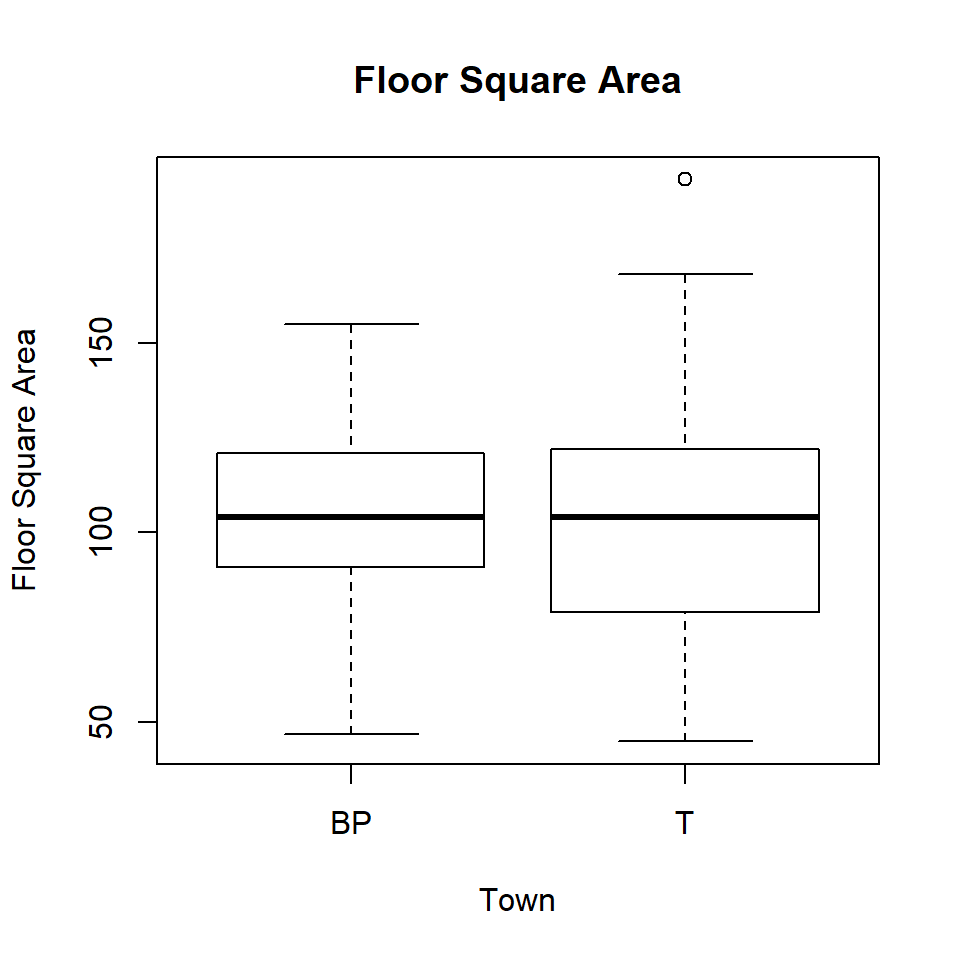
\includegraphics{bookdown-demo_files/figure-latex/unnamed-chunk-5-1.pdf}
\caption{\label{fig:unnamed-chunk-5}\label{fig:figs}Distance to MRT - BP
Town}
\end{figure}

\begin{Shaded}
\begin{Highlighting}[]
\KeywordTok{hist}\NormalTok{(data_tamp}\OperatorTok{$}\NormalTok{distance_mrt, }\DataTypeTok{main=}\StringTok{"Distance to MRT - T"}\NormalTok{, }\DataTypeTok{xlab=}\StringTok{"Distance to MRT"}\NormalTok{, }\DataTypeTok{ylab=}\StringTok{"Frequency"}\NormalTok{, }\DataTypeTok{breaks=}\KeywordTok{c}\NormalTok{(}\DecValTok{0}\NormalTok{,}\FloatTok{0.2}\NormalTok{,}\FloatTok{0.4}\NormalTok{,}\FloatTok{0.6}\NormalTok{,}\FloatTok{0.8}\NormalTok{,}\DecValTok{1}\NormalTok{,}\FloatTok{1.2}\NormalTok{,}\FloatTok{1.4}\NormalTok{,}\FloatTok{1.6}\NormalTok{,}\FloatTok{1.8}\NormalTok{,}\DecValTok{2}\NormalTok{,}\FloatTok{2.2}\NormalTok{))}
\end{Highlighting}
\end{Shaded}

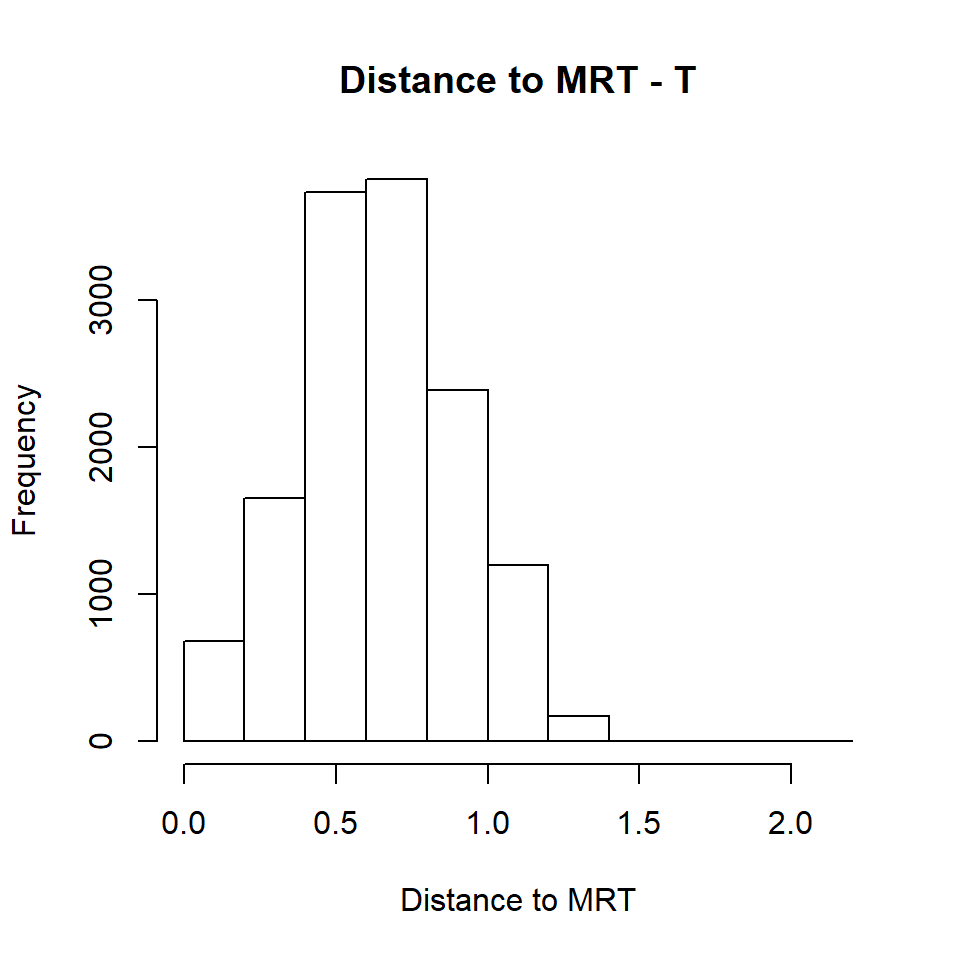
\includegraphics{bookdown-demo_files/figure-latex/unnamed-chunk-6-1.pdf}
The distance to MRT is summarised in the two histograms, with mean for
BP 1.02km and Tampines 0.64km. With three MRT stations are taken into
consideration, HDBs are nearer to MRt and hence a lower mean distance to
MRT. Hence, 0.4 to 0.8km range to MRT for Tampines is more common than 1
to 1.2km for BP.

\begin{Shaded}
\begin{Highlighting}[]
\KeywordTok{boxplot}\NormalTok{(data_bp}\OperatorTok{$}\NormalTok{floor_area_sqm,data_tamp}\OperatorTok{$}\NormalTok{floor_area_sqm, }\DataTypeTok{main=}\StringTok{"Floor Square Area"}\NormalTok{, }\DataTypeTok{xlab=}\StringTok{"Town"}\NormalTok{, }\DataTypeTok{ylab=}\StringTok{"Floor Square Area"}\NormalTok{, }\DataTypeTok{names=}\KeywordTok{c}\NormalTok{(}\StringTok{"BP"}\NormalTok{, }\StringTok{"T"}\NormalTok{))}
\end{Highlighting}
\end{Shaded}

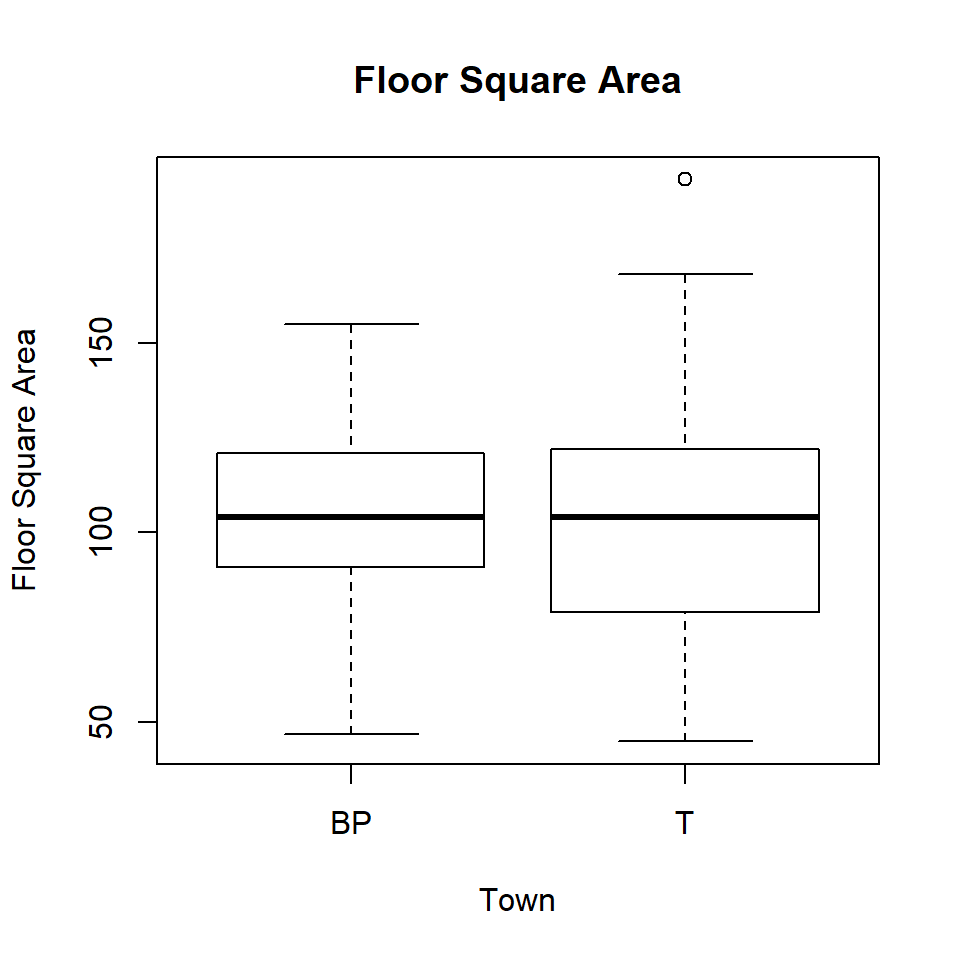
\includegraphics{bookdown-demo_files/figure-latex/unnamed-chunk-7-1.pdf}
Considering by each period, the mean resale price has increased and then
decreased for BP but it has increased throughout in Tampines. BP is a
non-matured town with more Built to Order flats coming up to ramp up the
supply, then it has seen a lower average price. Also, the resale market
also accounts for the other factors such as proximity to Central
Business District and attractiveness of the town.

\begin{Shaded}
\begin{Highlighting}[]
\KeywordTok{ggplot}\NormalTok{(}\DataTypeTok{data=}\NormalTok{data_bp, }\KeywordTok{aes}\NormalTok{(}\DataTypeTok{x=}\NormalTok{flat_type)) }\OperatorTok{+}
\StringTok{    }\KeywordTok{geom_bar}\NormalTok{(}\DataTypeTok{stat=}\StringTok{"count"}\NormalTok{) }\OperatorTok{+}\StringTok{ }\KeywordTok{ggtitle}\NormalTok{(}\StringTok{"BP by Flat Type"}\NormalTok{) }\OperatorTok{+}
\StringTok{    }\KeywordTok{theme_bw}\NormalTok{()}
\end{Highlighting}
\end{Shaded}

\begin{figure}
\centering
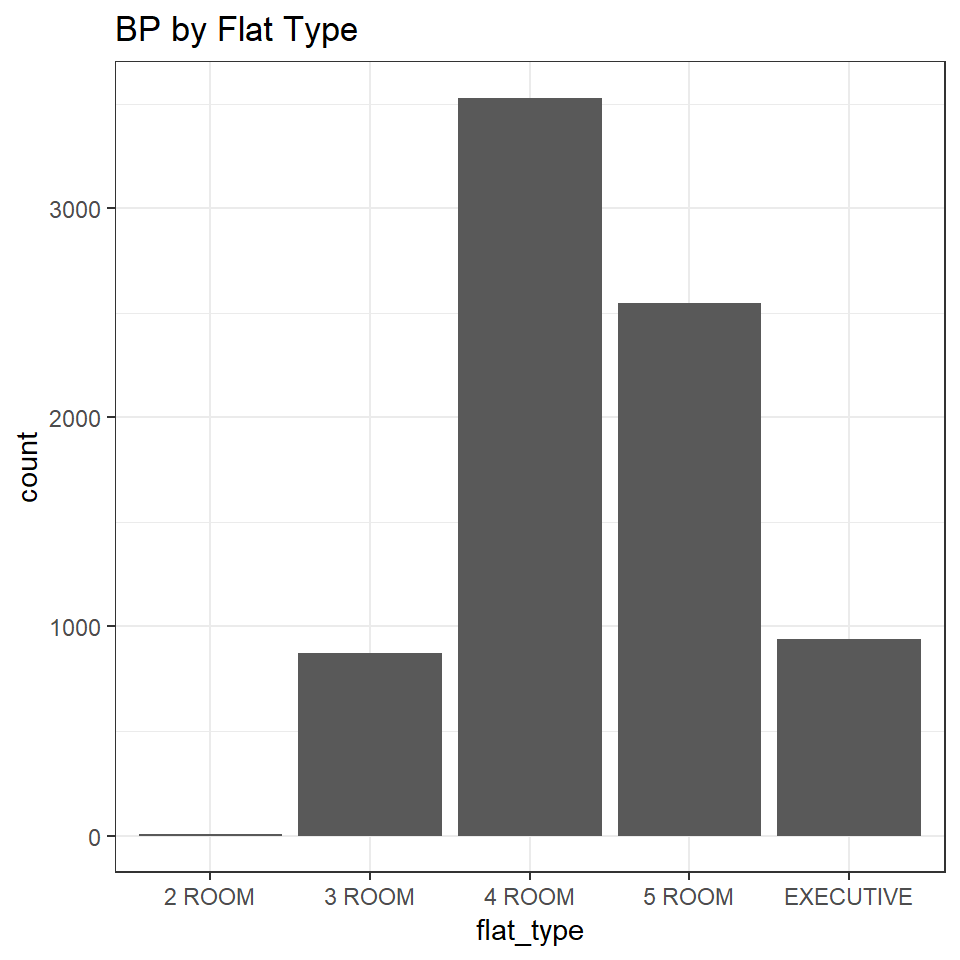
\includegraphics{bookdown-demo_files/figure-latex/unnamed-chunk-8-1.pdf}
\caption{\label{fig:unnamed-chunk-8}\label{fig:figs}BP by Flat Type}
\end{figure}

\begin{Shaded}
\begin{Highlighting}[]
\KeywordTok{ggplot}\NormalTok{(}\DataTypeTok{data=}\NormalTok{data_tamp, }\KeywordTok{aes}\NormalTok{(}\DataTypeTok{x=}\NormalTok{flat_type)) }\OperatorTok{+}
\StringTok{    }\KeywordTok{geom_bar}\NormalTok{(}\DataTypeTok{stat=}\StringTok{"count"}\NormalTok{) }\OperatorTok{+}\StringTok{ }\KeywordTok{ggtitle}\NormalTok{(}\StringTok{"T by Flat Type"}\NormalTok{) }\OperatorTok{+}
\StringTok{    }\KeywordTok{theme_bw}\NormalTok{()}
\end{Highlighting}
\end{Shaded}

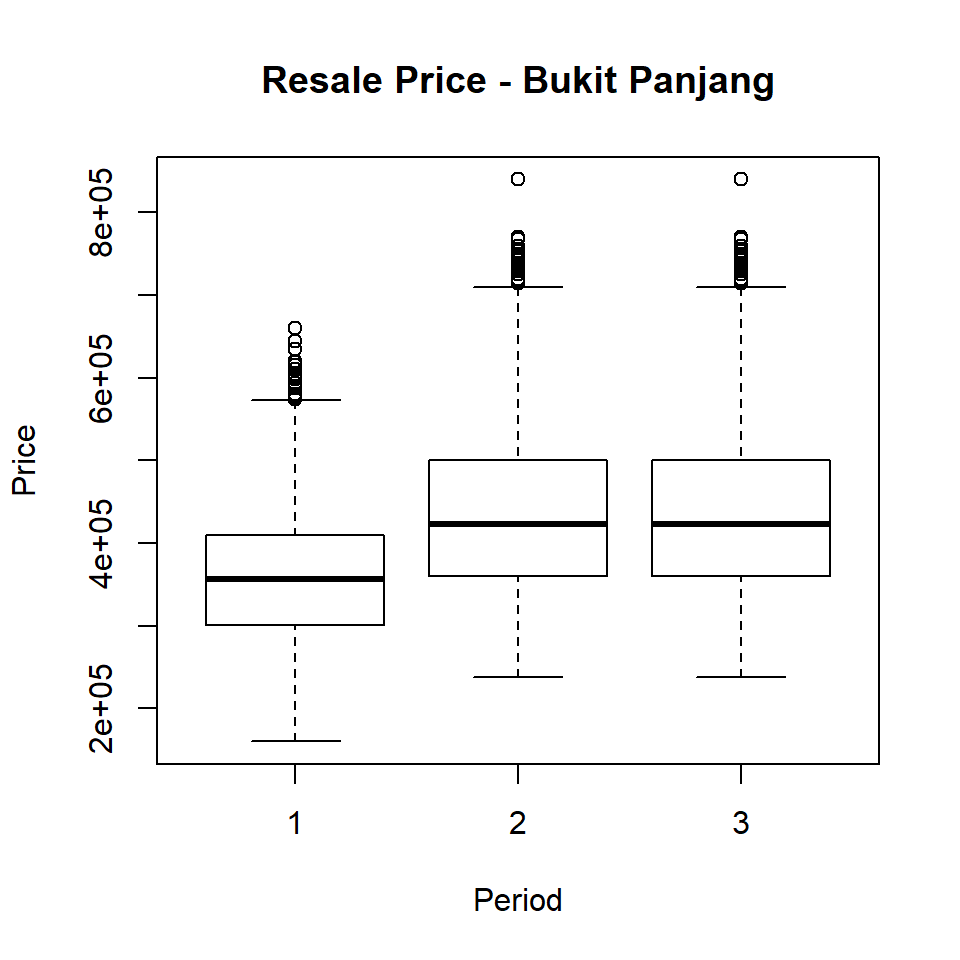
\includegraphics{bookdown-demo_files/figure-latex/unnamed-chunk-9-1.pdf}
By flat type, majority of the flats are 4-room 3530 units for BP and
5331 Tampines. This is typical of a HDB estate with 39\% and 45\% of the
HDB units 4 rooms which is the middle class. There is more 3 room in
Tampines which is contributed by a older generation of flats.

\begin{Shaded}
\begin{Highlighting}[]
\KeywordTok{boxplot}\NormalTok{(period1bp}\OperatorTok{$}\NormalTok{resale_price,period2bp}\OperatorTok{$}\NormalTok{resale_price,period2bp}\OperatorTok{$}\NormalTok{resale_price, }\DataTypeTok{main=}\StringTok{"Resale Price - Bukit Panjang"}\NormalTok{, }\DataTypeTok{xlab=}\StringTok{"Period"}\NormalTok{, }\DataTypeTok{ylab=}\StringTok{"Price"}\NormalTok{, }\DataTypeTok{names=}\KeywordTok{c}\NormalTok{(}\StringTok{"1"}\NormalTok{, }\StringTok{"2"}\NormalTok{,}\StringTok{"3"}\NormalTok{))}
\end{Highlighting}
\end{Shaded}

\begin{figure}
\centering
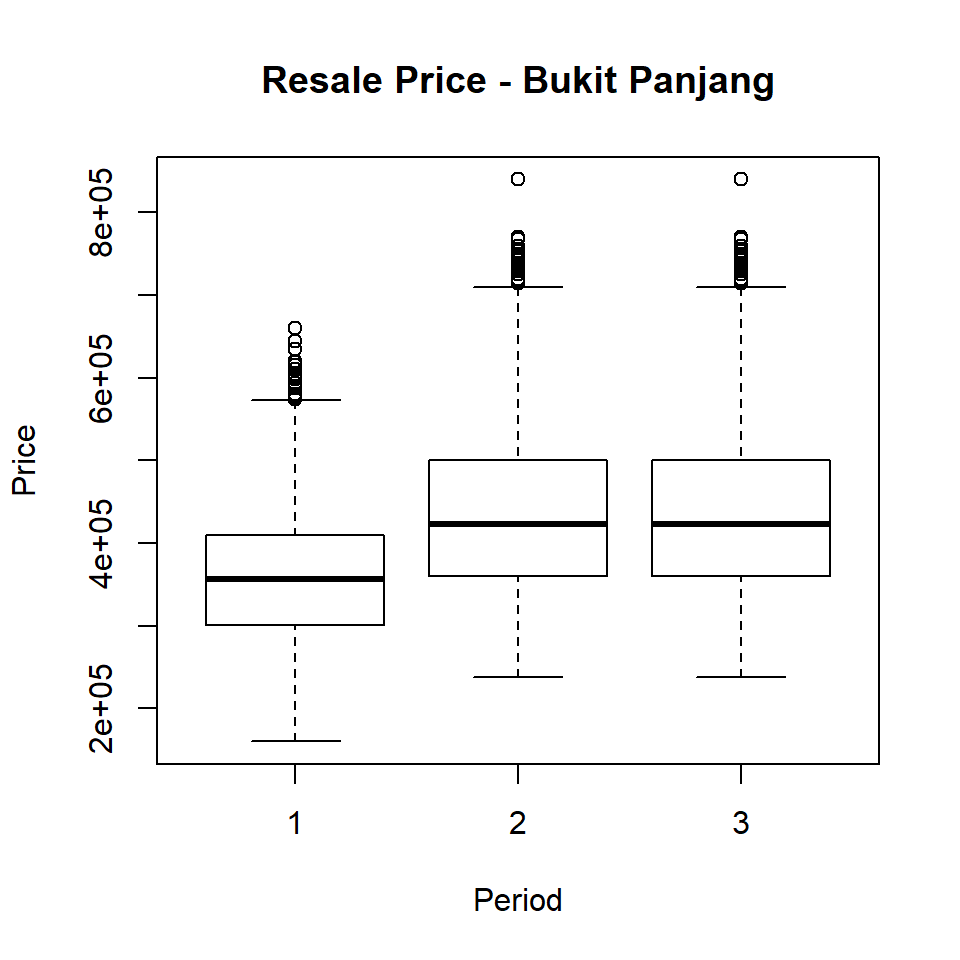
\includegraphics{bookdown-demo_files/figure-latex/unnamed-chunk-11-1.pdf}
\caption{\label{fig:unnamed-chunk-11}\label{fig:figs}Resale Price in BP}
\end{figure}

\begin{Shaded}
\begin{Highlighting}[]
\KeywordTok{boxplot}\NormalTok{(period1tamp}\OperatorTok{$}\NormalTok{resale_price,period2tamp}\OperatorTok{$}\NormalTok{resale_price,period2tamp}\OperatorTok{$}\NormalTok{resale_price, }\DataTypeTok{main=}\StringTok{"Resale Price - Tampines"}\NormalTok{, }\DataTypeTok{xlab=}\StringTok{"Period"}\NormalTok{, }\DataTypeTok{ylab=}\StringTok{"Price"}\NormalTok{, }\DataTypeTok{names=}\KeywordTok{c}\NormalTok{(}\StringTok{"1"}\NormalTok{, }\StringTok{"2"}\NormalTok{,}\StringTok{"3"}\NormalTok{))}
\end{Highlighting}
\end{Shaded}

\begin{figure}
\centering
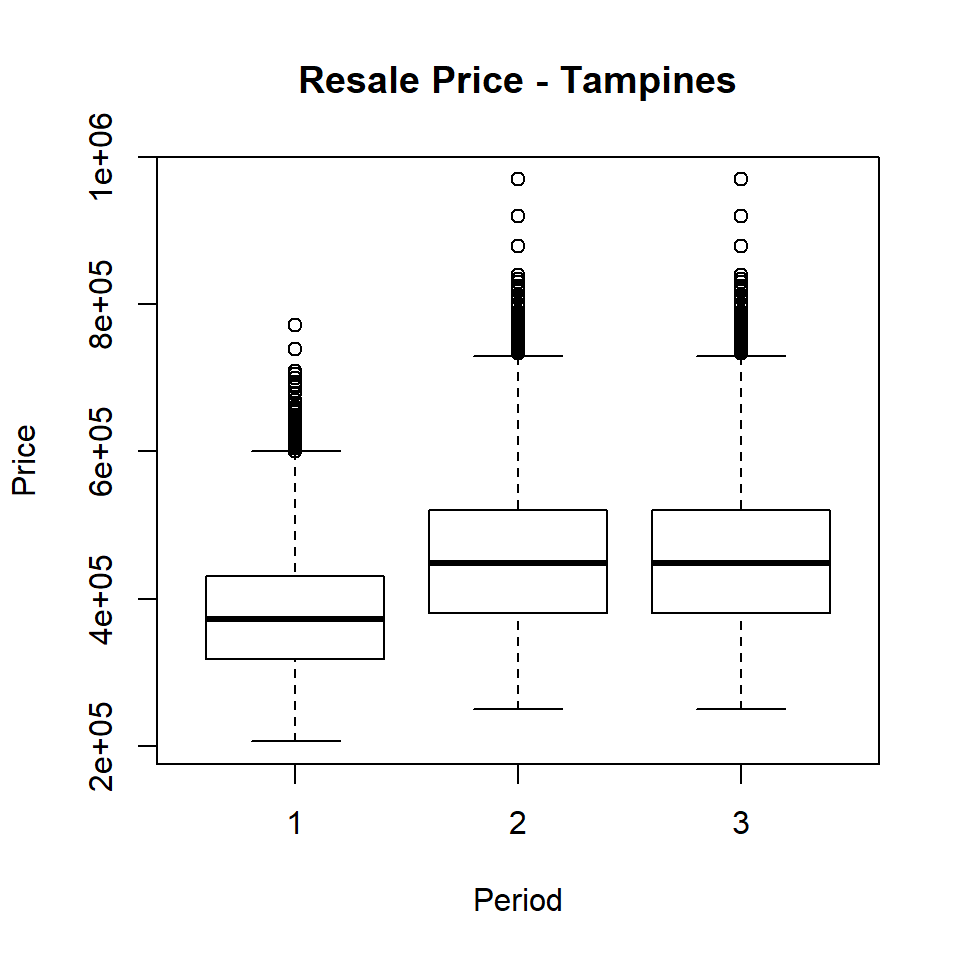
\includegraphics{bookdown-demo_files/figure-latex/unnamed-chunk-12-1.pdf}
\caption{\label{fig:unnamed-chunk-12}\label{fig:figs}Resale Price in T}
\end{figure}

The mean resale price for BP and T are \$409,776 and \$433,119 for all 3
periods. Looking at period-by-period, BP has increase from period 1 to 2
but a fall from period 2 to 3. Tampines has increased with a steeper
climb from period 1 to 2. Maisonette and other big flats that will fetch
prices much higher than the 3rd quartile.

\chapter{Method 1 - Regression}\label{method-1---regression}

Ordinary least squares linear regression is done firstly (Base Model) to
establish the relationship between the variables. Log-linear regression
is performed to determine the percentage change in resale price with
respect to the change in the independent variables (Change Model).

The assumptions to have a good model fit are:

\begin{enumerate}
\def\labelenumi{\arabic{enumi}.}
\item
  Variables are independently distributed
\item
  No multi-collinearity
\item
  Large outliers are rare
\end{enumerate}

\section{Linear Regression Model}\label{linear-regression-model}

\subsection{Coefficients}\label{coefficients}

\begin{longtable}[]{@{}llll@{}}
\toprule
\begin{minipage}[b]{0.18\columnwidth}\raggedright\strut
\strut
\end{minipage} & \begin{minipage}[b]{0.24\columnwidth}\raggedright\strut
\strut
\end{minipage} & \begin{minipage}[b]{0.24\columnwidth}\raggedright\strut
Dependent variable:\strut
\end{minipage} & \begin{minipage}[b]{0.22\columnwidth}\raggedright\strut
\strut
\end{minipage}\tabularnewline
\midrule
\endhead
\begin{minipage}[t]{0.18\columnwidth}\raggedright\strut
\strut
\end{minipage} & \begin{minipage}[t]{0.24\columnwidth}\raggedright\strut
\strut
\end{minipage} & \begin{minipage}[t]{0.24\columnwidth}\raggedright\strut
\strut
\end{minipage} & \begin{minipage}[t]{0.22\columnwidth}\raggedright\strut
\strut
\end{minipage}\tabularnewline
\begin{minipage}[t]{0.18\columnwidth}\raggedright\strut
\strut
\end{minipage} & \begin{minipage}[t]{0.24\columnwidth}\raggedright\strut
\strut
\end{minipage} & \begin{minipage}[t]{0.24\columnwidth}\raggedright\strut
resale\_price\strut
\end{minipage} & \begin{minipage}[t]{0.22\columnwidth}\raggedright\strut
\strut
\end{minipage}\tabularnewline
\begin{minipage}[t]{0.18\columnwidth}\raggedright\strut
\strut
\end{minipage} & \begin{minipage}[t]{0.24\columnwidth}\raggedright\strut
BP period 1\strut
\end{minipage} & \begin{minipage}[t]{0.24\columnwidth}\raggedright\strut
BP period 2\strut
\end{minipage} & \begin{minipage}[t]{0.22\columnwidth}\raggedright\strut
BP period 3\strut
\end{minipage}\tabularnewline
\begin{minipage}[t]{0.18\columnwidth}\raggedright\strut
\strut
\end{minipage} & \begin{minipage}[t]{0.24\columnwidth}\raggedright\strut
\strut
\end{minipage} & \begin{minipage}[t]{0.24\columnwidth}\raggedright\strut
\strut
\end{minipage} & \begin{minipage}[t]{0.22\columnwidth}\raggedright\strut
\strut
\end{minipage}\tabularnewline
\begin{minipage}[t]{0.18\columnwidth}\raggedright\strut
floor\_area\_sqm\strut
\end{minipage} & \begin{minipage}[t]{0.24\columnwidth}\raggedright\strut
2,689.456***\strut
\end{minipage} & \begin{minipage}[t]{0.24\columnwidth}\raggedright\strut
3,575.292***\strut
\end{minipage} & \begin{minipage}[t]{0.22\columnwidth}\raggedright\strut
4,297.322***\strut
\end{minipage}\tabularnewline
\begin{minipage}[t]{0.18\columnwidth}\raggedright\strut
\strut
\end{minipage} & \begin{minipage}[t]{0.24\columnwidth}\raggedright\strut
(47.462)\strut
\end{minipage} & \begin{minipage}[t]{0.24\columnwidth}\raggedright\strut
(36.961)\strut
\end{minipage} & \begin{minipage}[t]{0.22\columnwidth}\raggedright\strut
(86.110)\strut
\end{minipage}\tabularnewline
\begin{minipage}[t]{0.18\columnwidth}\raggedright\strut
\strut
\end{minipage} & \begin{minipage}[t]{0.24\columnwidth}\raggedright\strut
\strut
\end{minipage} & \begin{minipage}[t]{0.24\columnwidth}\raggedright\strut
\strut
\end{minipage} & \begin{minipage}[t]{0.22\columnwidth}\raggedright\strut
\strut
\end{minipage}\tabularnewline
\begin{minipage}[t]{0.18\columnwidth}\raggedright\strut
connected\strut
\end{minipage} & \begin{minipage}[t]{0.24\columnwidth}\raggedright\strut
22,194.180***\strut
\end{minipage} & \begin{minipage}[t]{0.24\columnwidth}\raggedright\strut
41,669.390***\strut
\end{minipage} & \begin{minipage}[t]{0.22\columnwidth}\raggedright\strut
61,123.180***\strut
\end{minipage}\tabularnewline
\begin{minipage}[t]{0.18\columnwidth}\raggedright\strut
\strut
\end{minipage} & \begin{minipage}[t]{0.24\columnwidth}\raggedright\strut
(1,808.657)\strut
\end{minipage} & \begin{minipage}[t]{0.24\columnwidth}\raggedright\strut
(1,431.850)\strut
\end{minipage} & \begin{minipage}[t]{0.22\columnwidth}\raggedright\strut
(3,403.679)\strut
\end{minipage}\tabularnewline
\begin{minipage}[t]{0.18\columnwidth}\raggedright\strut
\strut
\end{minipage} & \begin{minipage}[t]{0.24\columnwidth}\raggedright\strut
\strut
\end{minipage} & \begin{minipage}[t]{0.24\columnwidth}\raggedright\strut
\strut
\end{minipage} & \begin{minipage}[t]{0.22\columnwidth}\raggedright\strut
\strut
\end{minipage}\tabularnewline
\begin{minipage}[t]{0.18\columnwidth}\raggedright\strut
lease\_remaining\strut
\end{minipage} & \begin{minipage}[t]{0.24\columnwidth}\raggedright\strut
3,321.929***\strut
\end{minipage} & \begin{minipage}[t]{0.24\columnwidth}\raggedright\strut
3,777.677***\strut
\end{minipage} & \begin{minipage}[t]{0.22\columnwidth}\raggedright\strut
3,645.197***\strut
\end{minipage}\tabularnewline
\begin{minipage}[t]{0.18\columnwidth}\raggedright\strut
\strut
\end{minipage} & \begin{minipage}[t]{0.24\columnwidth}\raggedright\strut
(154.635)\strut
\end{minipage} & \begin{minipage}[t]{0.24\columnwidth}\raggedright\strut
(112.449)\strut
\end{minipage} & \begin{minipage}[t]{0.22\columnwidth}\raggedright\strut
(244.210)\strut
\end{minipage}\tabularnewline
\begin{minipage}[t]{0.18\columnwidth}\raggedright\strut
\strut
\end{minipage} & \begin{minipage}[t]{0.24\columnwidth}\raggedright\strut
\strut
\end{minipage} & \begin{minipage}[t]{0.24\columnwidth}\raggedright\strut
\strut
\end{minipage} & \begin{minipage}[t]{0.22\columnwidth}\raggedright\strut
\strut
\end{minipage}\tabularnewline
\begin{minipage}[t]{0.18\columnwidth}\raggedright\strut
storey\strut
\end{minipage} & \begin{minipage}[t]{0.24\columnwidth}\raggedright\strut
3,033.051***\strut
\end{minipage} & \begin{minipage}[t]{0.24\columnwidth}\raggedright\strut
3,851.335***\strut
\end{minipage} & \begin{minipage}[t]{0.22\columnwidth}\raggedright\strut
4,226.184***\strut
\end{minipage}\tabularnewline
\begin{minipage}[t]{0.18\columnwidth}\raggedright\strut
\strut
\end{minipage} & \begin{minipage}[t]{0.24\columnwidth}\raggedright\strut
(153.964)\strut
\end{minipage} & \begin{minipage}[t]{0.24\columnwidth}\raggedright\strut
(125.236)\strut
\end{minipage} & \begin{minipage}[t]{0.22\columnwidth}\raggedright\strut
(284.796)\strut
\end{minipage}\tabularnewline
\begin{minipage}[t]{0.18\columnwidth}\raggedright\strut
\strut
\end{minipage} & \begin{minipage}[t]{0.24\columnwidth}\raggedright\strut
\strut
\end{minipage} & \begin{minipage}[t]{0.24\columnwidth}\raggedright\strut
\strut
\end{minipage} & \begin{minipage}[t]{0.22\columnwidth}\raggedright\strut
\strut
\end{minipage}\tabularnewline
\begin{minipage}[t]{0.18\columnwidth}\raggedright\strut
Constant\strut
\end{minipage} & \begin{minipage}[t]{0.24\columnwidth}\raggedright\strut
-241,824.200***\strut
\end{minipage} & \begin{minipage}[t]{0.24\columnwidth}\raggedright\strut
-297,502.400***\strut
\end{minipage} & \begin{minipage}[t]{0.22\columnwidth}\raggedright\strut
-381,081.600***\strut
\end{minipage}\tabularnewline
\begin{minipage}[t]{0.18\columnwidth}\raggedright\strut
\strut
\end{minipage} & \begin{minipage}[t]{0.24\columnwidth}\raggedright\strut
(13,006.660)\strut
\end{minipage} & \begin{minipage}[t]{0.24\columnwidth}\raggedright\strut
(9,177.533)\strut
\end{minipage} & \begin{minipage}[t]{0.22\columnwidth}\raggedright\strut
(21,795.130)\strut
\end{minipage}\tabularnewline
\begin{minipage}[t]{0.18\columnwidth}\raggedright\strut
\strut
\end{minipage} & \begin{minipage}[t]{0.24\columnwidth}\raggedright\strut
\strut
\end{minipage} & \begin{minipage}[t]{0.24\columnwidth}\raggedright\strut
\strut
\end{minipage} & \begin{minipage}[t]{0.22\columnwidth}\raggedright\strut
\strut
\end{minipage}\tabularnewline
\begin{minipage}[t]{0.18\columnwidth}\raggedright\strut
\strut
\end{minipage} & \begin{minipage}[t]{0.24\columnwidth}\raggedright\strut
\strut
\end{minipage} & \begin{minipage}[t]{0.24\columnwidth}\raggedright\strut
\strut
\end{minipage} & \begin{minipage}[t]{0.22\columnwidth}\raggedright\strut
\strut
\end{minipage}\tabularnewline
\begin{minipage}[t]{0.18\columnwidth}\raggedright\strut
Observations\strut
\end{minipage} & \begin{minipage}[t]{0.24\columnwidth}\raggedright\strut
2,784\strut
\end{minipage} & \begin{minipage}[t]{0.24\columnwidth}\raggedright\strut
4,240\strut
\end{minipage} & \begin{minipage}[t]{0.22\columnwidth}\raggedright\strut
873\strut
\end{minipage}\tabularnewline
\begin{minipage}[t]{0.18\columnwidth}\raggedright\strut
R2\strut
\end{minipage} & \begin{minipage}[t]{0.24\columnwidth}\raggedright\strut
0.663\strut
\end{minipage} & \begin{minipage}[t]{0.24\columnwidth}\raggedright\strut
0.782\strut
\end{minipage} & \begin{minipage}[t]{0.22\columnwidth}\raggedright\strut
0.805\strut
\end{minipage}\tabularnewline
\begin{minipage}[t]{0.18\columnwidth}\raggedright\strut
Adjusted R2\strut
\end{minipage} & \begin{minipage}[t]{0.24\columnwidth}\raggedright\strut
0.663\strut
\end{minipage} & \begin{minipage}[t]{0.24\columnwidth}\raggedright\strut
0.782\strut
\end{minipage} & \begin{minipage}[t]{0.22\columnwidth}\raggedright\strut
0.804\strut
\end{minipage}\tabularnewline
\begin{minipage}[t]{0.18\columnwidth}\raggedright\strut
Residual Std. Error\strut
\end{minipage} & \begin{minipage}[t]{0.24\columnwidth}\raggedright\strut
46,918.500 (df = 2779)\strut
\end{minipage} & \begin{minipage}[t]{0.24\columnwidth}\raggedright\strut
45,808.740 (df = 4235)\strut
\end{minipage} & \begin{minipage}[t]{0.22\columnwidth}\raggedright\strut
49,183.120 (df = 868)\strut
\end{minipage}\tabularnewline
\begin{minipage}[t]{0.18\columnwidth}\raggedright\strut
F Statistic\strut
\end{minipage} & \begin{minipage}[t]{0.24\columnwidth}\raggedright\strut
1,367.588*** (df = 4; 2779)\strut
\end{minipage} & \begin{minipage}[t]{0.24\columnwidth}\raggedright\strut
3,805.884*** (df = 4; 4235)\strut
\end{minipage} & \begin{minipage}[t]{0.22\columnwidth}\raggedright\strut
895.464*** (df = 4; 868)\strut
\end{minipage}\tabularnewline
\bottomrule
\end{longtable}

Note: *p\textless{}0.1; **p\textless{}0.05; ***p\textless{}0.01

The coefficients for connected is positive that is correctly predicted
as houses nearer to MRT command a higher price. All coefficients are
p-value\textless{}0.01 that shows a good way to estimate the effect. The
constant has dropped significantly which may be prone to omitted
variable bias. R-squared is not good for period 1 while period 2 and
period 3 is high. Taking an example of a flat with floor area 100 square
metres, storey 7, with lease remaining at 80,

\begin{longtable}[]{@{}llll@{}}
\toprule
& Period 1 & Period 2 & Period 3\tabularnewline
\midrule
\endhead
Connected & 336,301 & 430,869 & 430,972\tabularnewline
Not connected & 314,107 & 389,200 & 369,849\tabularnewline
\bottomrule
\end{longtable}

This illustrates that there is additional benefit of staying near Bukit
Panjang MRT. The stabilisation of period 2 and period 3 can be
attributed to increase in number of Build to Order flats. As the
transactions are not homogenous and certain flat type or flat size may
be transacted so the data may be skewed.

\begin{longtable}[]{@{}llll@{}}
\toprule
\begin{minipage}[b]{0.17\columnwidth}\raggedright\strut
\strut
\end{minipage} & \begin{minipage}[b]{0.24\columnwidth}\raggedright\strut
\strut
\end{minipage} & \begin{minipage}[b]{0.24\columnwidth}\raggedright\strut
Dependent Variable\strut
\end{minipage} & \begin{minipage}[b]{0.24\columnwidth}\raggedright\strut
\strut
\end{minipage}\tabularnewline
\midrule
\endhead
\begin{minipage}[t]{0.17\columnwidth}\raggedright\strut
\strut
\end{minipage} & \begin{minipage}[t]{0.24\columnwidth}\raggedright\strut
\strut
\end{minipage} & \begin{minipage}[t]{0.24\columnwidth}\raggedright\strut
\strut
\end{minipage} & \begin{minipage}[t]{0.24\columnwidth}\raggedright\strut
\strut
\end{minipage}\tabularnewline
\begin{minipage}[t]{0.17\columnwidth}\raggedright\strut
\strut
\end{minipage} & \begin{minipage}[t]{0.24\columnwidth}\raggedright\strut
\strut
\end{minipage} & \begin{minipage}[t]{0.24\columnwidth}\raggedright\strut
resale\_price\strut
\end{minipage} & \begin{minipage}[t]{0.24\columnwidth}\raggedright\strut
\strut
\end{minipage}\tabularnewline
\begin{minipage}[t]{0.17\columnwidth}\raggedright\strut
\strut
\end{minipage} & \begin{minipage}[t]{0.24\columnwidth}\raggedright\strut
T period 1\strut
\end{minipage} & \begin{minipage}[t]{0.24\columnwidth}\raggedright\strut
T period 2\strut
\end{minipage} & \begin{minipage}[t]{0.24\columnwidth}\raggedright\strut
T period 3\strut
\end{minipage}\tabularnewline
\begin{minipage}[t]{0.17\columnwidth}\raggedright\strut
\strut
\end{minipage} & \begin{minipage}[t]{0.24\columnwidth}\raggedright\strut
\strut
\end{minipage} & \begin{minipage}[t]{0.24\columnwidth}\raggedright\strut
\strut
\end{minipage} & \begin{minipage}[t]{0.24\columnwidth}\raggedright\strut
\strut
\end{minipage}\tabularnewline
\begin{minipage}[t]{0.17\columnwidth}\raggedright\strut
floor\_area\_sqm\strut
\end{minipage} & \begin{minipage}[t]{0.24\columnwidth}\raggedright\strut
3,036.943***\strut
\end{minipage} & \begin{minipage}[t]{0.24\columnwidth}\raggedright\strut
3,729.498***\strut
\end{minipage} & \begin{minipage}[t]{0.24\columnwidth}\raggedright\strut
4,294.834***\strut
\end{minipage}\tabularnewline
\begin{minipage}[t]{0.17\columnwidth}\raggedright\strut
\strut
\end{minipage} & \begin{minipage}[t]{0.24\columnwidth}\raggedright\strut
(28.858)\strut
\end{minipage} & \begin{minipage}[t]{0.24\columnwidth}\raggedright\strut
(25.294)\strut
\end{minipage} & \begin{minipage}[t]{0.24\columnwidth}\raggedright\strut
(58.870)\strut
\end{minipage}\tabularnewline
\begin{minipage}[t]{0.17\columnwidth}\raggedright\strut
\strut
\end{minipage} & \begin{minipage}[t]{0.24\columnwidth}\raggedright\strut
\strut
\end{minipage} & \begin{minipage}[t]{0.24\columnwidth}\raggedright\strut
\strut
\end{minipage} & \begin{minipage}[t]{0.24\columnwidth}\raggedright\strut
\strut
\end{minipage}\tabularnewline
\begin{minipage}[t]{0.17\columnwidth}\raggedright\strut
connected\strut
\end{minipage} & \begin{minipage}[t]{0.24\columnwidth}\raggedright\strut
2,016.711\strut
\end{minipage} & \begin{minipage}[t]{0.24\columnwidth}\raggedright\strut
19,151.510***\strut
\end{minipage} & \begin{minipage}[t]{0.24\columnwidth}\raggedright\strut
27,530.090***\strut
\end{minipage}\tabularnewline
\begin{minipage}[t]{0.17\columnwidth}\raggedright\strut
\strut
\end{minipage} & \begin{minipage}[t]{0.24\columnwidth}\raggedright\strut
(2,063.843)\strut
\end{minipage} & \begin{minipage}[t]{0.24\columnwidth}\raggedright\strut
(1,817.018)\strut
\end{minipage} & \begin{minipage}[t]{0.24\columnwidth}\raggedright\strut
(4,927.825)\strut
\end{minipage}\tabularnewline
\begin{minipage}[t]{0.17\columnwidth}\raggedright\strut
\strut
\end{minipage} & \begin{minipage}[t]{0.24\columnwidth}\raggedright\strut
\strut
\end{minipage} & \begin{minipage}[t]{0.24\columnwidth}\raggedright\strut
\strut
\end{minipage} & \begin{minipage}[t]{0.24\columnwidth}\raggedright\strut
\strut
\end{minipage}\tabularnewline
\begin{minipage}[t]{0.17\columnwidth}\raggedright\strut
lease\_remaining\strut
\end{minipage} & \begin{minipage}[t]{0.24\columnwidth}\raggedright\strut
-1,009.607***\strut
\end{minipage} & \begin{minipage}[t]{0.24\columnwidth}\raggedright\strut
2,034.100***\strut
\end{minipage} & \begin{minipage}[t]{0.24\columnwidth}\raggedright\strut
1,131.236***\strut
\end{minipage}\tabularnewline
\begin{minipage}[t]{0.17\columnwidth}\raggedright\strut
\strut
\end{minipage} & \begin{minipage}[t]{0.24\columnwidth}\raggedright\strut
(141.440)\strut
\end{minipage} & \begin{minipage}[t]{0.24\columnwidth}\raggedright\strut
(103.722)\strut
\end{minipage} & \begin{minipage}[t]{0.24\columnwidth}\raggedright\strut
(240.352)\strut
\end{minipage}\tabularnewline
\begin{minipage}[t]{0.17\columnwidth}\raggedright\strut
\strut
\end{minipage} & \begin{minipage}[t]{0.24\columnwidth}\raggedright\strut
\strut
\end{minipage} & \begin{minipage}[t]{0.24\columnwidth}\raggedright\strut
\strut
\end{minipage} & \begin{minipage}[t]{0.24\columnwidth}\raggedright\strut
\strut
\end{minipage}\tabularnewline
\begin{minipage}[t]{0.17\columnwidth}\raggedright\strut
storey\strut
\end{minipage} & \begin{minipage}[t]{0.24\columnwidth}\raggedright\strut
2,828.676***\strut
\end{minipage} & \begin{minipage}[t]{0.24\columnwidth}\raggedright\strut
3,997.770***\strut
\end{minipage} & \begin{minipage}[t]{0.24\columnwidth}\raggedright\strut
4,829.908***\strut
\end{minipage}\tabularnewline
\begin{minipage}[t]{0.17\columnwidth}\raggedright\strut
\strut
\end{minipage} & \begin{minipage}[t]{0.24\columnwidth}\raggedright\strut
(187.757)\strut
\end{minipage} & \begin{minipage}[t]{0.24\columnwidth}\raggedright\strut
(163.370)\strut
\end{minipage} & \begin{minipage}[t]{0.24\columnwidth}\raggedright\strut
(442.000)\strut
\end{minipage}\tabularnewline
\begin{minipage}[t]{0.17\columnwidth}\raggedright\strut
\strut
\end{minipage} & \begin{minipage}[t]{0.24\columnwidth}\raggedright\strut
\strut
\end{minipage} & \begin{minipage}[t]{0.24\columnwidth}\raggedright\strut
\strut
\end{minipage} & \begin{minipage}[t]{0.24\columnwidth}\raggedright\strut
\strut
\end{minipage}\tabularnewline
\begin{minipage}[t]{0.17\columnwidth}\raggedright\strut
Constant\strut
\end{minipage} & \begin{minipage}[t]{0.24\columnwidth}\raggedright\strut
125,626.900***\strut
\end{minipage} & \begin{minipage}[t]{0.24\columnwidth}\raggedright\strut
-115,154.200***\strut
\end{minipage} & \begin{minipage}[t]{0.24\columnwidth}\raggedright\strut
-123,982.500***\strut
\end{minipage}\tabularnewline
\begin{minipage}[t]{0.17\columnwidth}\raggedright\strut
\strut
\end{minipage} & \begin{minipage}[t]{0.24\columnwidth}\raggedright\strut
(10,348.700)\strut
\end{minipage} & \begin{minipage}[t]{0.24\columnwidth}\raggedright\strut
(7,293.582)\strut
\end{minipage} & \begin{minipage}[t]{0.24\columnwidth}\raggedright\strut
(18,006.770)\strut
\end{minipage}\tabularnewline
\begin{minipage}[t]{0.17\columnwidth}\raggedright\strut
\strut
\end{minipage} & \begin{minipage}[t]{0.24\columnwidth}\raggedright\strut
\strut
\end{minipage} & \begin{minipage}[t]{0.24\columnwidth}\raggedright\strut
\strut
\end{minipage} & \begin{minipage}[t]{0.24\columnwidth}\raggedright\strut
\strut
\end{minipage}\tabularnewline
\begin{minipage}[t]{0.17\columnwidth}\raggedright\strut
\strut
\end{minipage} & \begin{minipage}[t]{0.24\columnwidth}\raggedright\strut
\strut
\end{minipage} & \begin{minipage}[t]{0.24\columnwidth}\raggedright\strut
\strut
\end{minipage} & \begin{minipage}[t]{0.24\columnwidth}\raggedright\strut
\strut
\end{minipage}\tabularnewline
\begin{minipage}[t]{0.17\columnwidth}\raggedright\strut
Observations\strut
\end{minipage} & \begin{minipage}[t]{0.24\columnwidth}\raggedright\strut
5,161\strut
\end{minipage} & \begin{minipage}[t]{0.24\columnwidth}\raggedright\strut
7,067\strut
\end{minipage} & \begin{minipage}[t]{0.24\columnwidth}\raggedright\strut
1,414\strut
\end{minipage}\tabularnewline
\begin{minipage}[t]{0.17\columnwidth}\raggedright\strut
R2\strut
\end{minipage} & \begin{minipage}[t]{0.24\columnwidth}\raggedright\strut
0.723\strut
\end{minipage} & \begin{minipage}[t]{0.24\columnwidth}\raggedright\strut
0.807\strut
\end{minipage} & \begin{minipage}[t]{0.24\columnwidth}\raggedright\strut
0.803\strut
\end{minipage}\tabularnewline
\begin{minipage}[t]{0.17\columnwidth}\raggedright\strut
Adjusted R2\strut
\end{minipage} & \begin{minipage}[t]{0.24\columnwidth}\raggedright\strut
0.723\strut
\end{minipage} & \begin{minipage}[t]{0.24\columnwidth}\raggedright\strut
0.807\strut
\end{minipage} & \begin{minipage}[t]{0.24\columnwidth}\raggedright\strut
0.802\strut
\end{minipage}\tabularnewline
\begin{minipage}[t]{0.17\columnwidth}\raggedright\strut
Residual Std. Error\strut
\end{minipage} & \begin{minipage}[t]{0.24\columnwidth}\raggedright\strut
45,863.240 (df = 5156)\strut
\end{minipage} & \begin{minipage}[t]{0.24\columnwidth}\raggedright\strut
47,581.530 (df = 7062)\strut
\end{minipage} & \begin{minipage}[t]{0.24\columnwidth}\raggedright\strut
57,127.880 (df = 1409)\strut
\end{minipage}\tabularnewline
\begin{minipage}[t]{0.17\columnwidth}\raggedright\strut
F Statistic\strut
\end{minipage} & \begin{minipage}[t]{0.24\columnwidth}\raggedright\strut
3,367.789*** (df = 4; 5156)\strut
\end{minipage} & \begin{minipage}[t]{0.24\columnwidth}\raggedright\strut
7,395.560*** (df = 4; 7062)\strut
\end{minipage} & \begin{minipage}[t]{0.24\columnwidth}\raggedright\strut
1,433.155*** (df = 4; 1409)\strut
\end{minipage}\tabularnewline
\bottomrule
\end{longtable}

Note: *p\textless{}0.1; **p\textless{}0.05; ***p\textless{}0.01

The coefficients for connected is positive that is the same for BP.
R-square is high which shows that the model is a good fit to predict
housing prices. The constant has decreased from period 1 to period 2
could be countered due to lease\_remaining parameter increased. Taking
the same attributes for illustration,

\begin{longtable}[]{@{}llll@{}}
\toprule
& Period 1 & Period 2 & Period 3\tabularnewline
\midrule
\endhead
Connected & 370,370 & 467,659 & 457,339\tabularnewline
Not connected & 368,353 & 448,508 & 429,809\tabularnewline
\bottomrule
\end{longtable}

The same trend for a fall from period 2 and period 3 is seen. The
premium of locating near MRT after construction seemed to stabilise
after a big jump after announcement. Notably, period 1 connected and not
connected are very close, as the coefficient is \$2016. This is useful
to see the increment of price by isolating the connected variable.

\subsection{Residuals}\label{residuals}

\begin{Shaded}
\begin{Highlighting}[]
\NormalTok{bp_ols_p1_re <-}\StringTok{ }\KeywordTok{augment}\NormalTok{(bp_ols_p1, }\DataTypeTok{data =}\NormalTok{ data_bp_p1)}
\NormalTok{bp_ols_p1_re }\OperatorTok\StringTok{ }
\StringTok{  }\KeywordTok{ggplot}\NormalTok{(}\KeywordTok{aes}\NormalTok{(}\DataTypeTok{x =}\NormalTok{ .resid)) }\OperatorTok{+}
\StringTok{  }\KeywordTok{geom_histogram}\NormalTok{(}\DataTypeTok{bins =} \DecValTok{50}\NormalTok{) }\OperatorTok{+}\StringTok{ }\KeywordTok{labs}\NormalTok{(}\DataTypeTok{title =} \StringTok{"Residuals Base Model BP Period 1"}\NormalTok{)}
\end{Highlighting}
\end{Shaded}

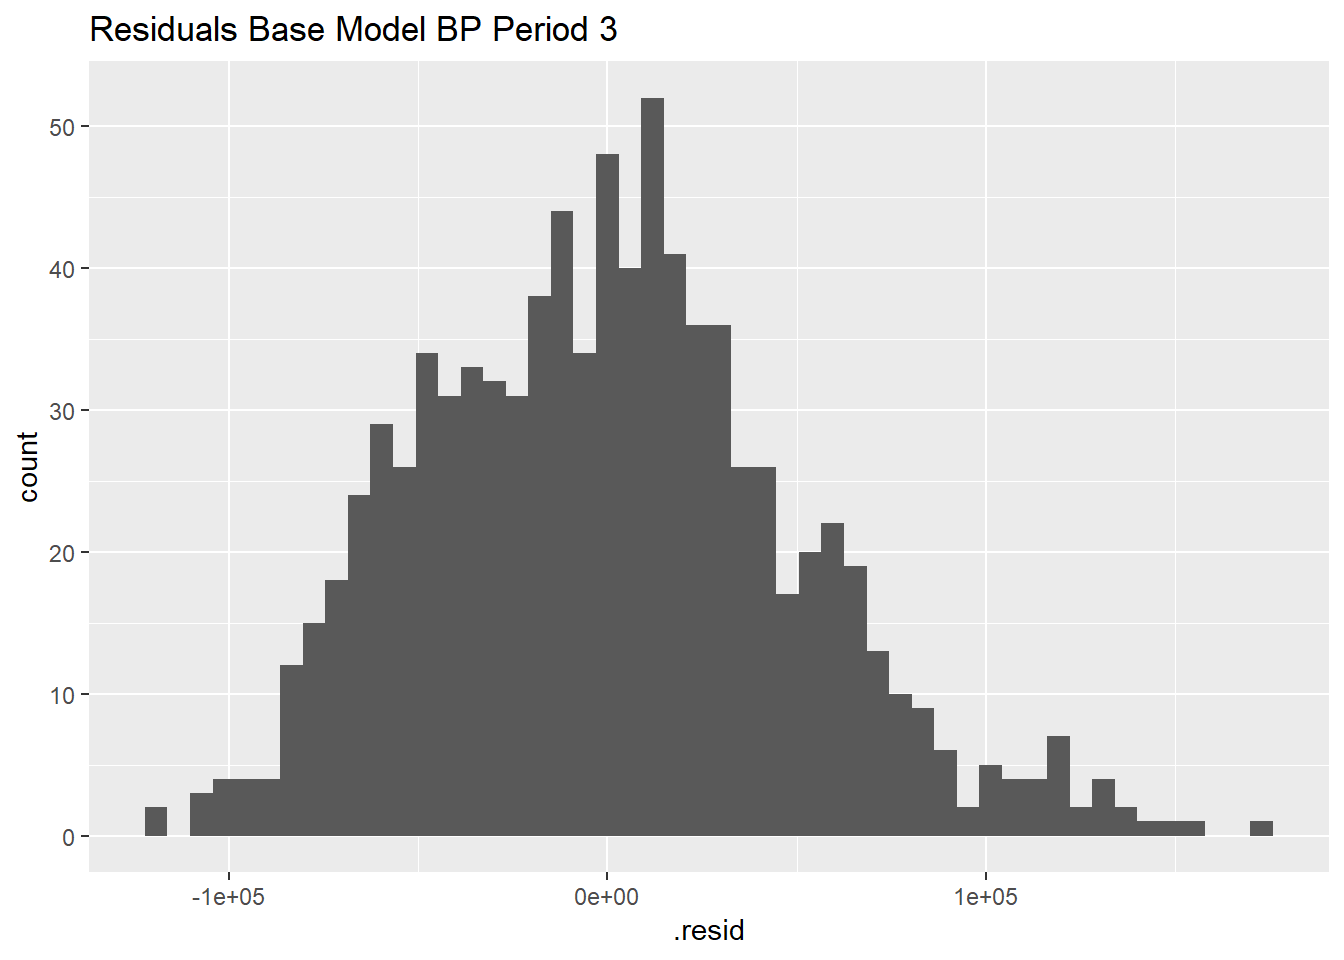
\includegraphics{bookdown-demo_files/figure-latex/unnamed-chunk-18-1.pdf}

\begin{Shaded}
\begin{Highlighting}[]
\NormalTok{bp_ols_p2_re <-}\StringTok{ }\KeywordTok{augment}\NormalTok{(bp_ols_p2, }\DataTypeTok{data =}\NormalTok{ data_bp_p2)}
\NormalTok{bp_ols_p2_re }\OperatorTok\StringTok{ }
\StringTok{  }\KeywordTok{ggplot}\NormalTok{(}\KeywordTok{aes}\NormalTok{(}\DataTypeTok{x =}\NormalTok{ .resid)) }\OperatorTok{+}
\StringTok{  }\KeywordTok{geom_histogram}\NormalTok{(}\DataTypeTok{bins =} \DecValTok{50}\NormalTok{) }\OperatorTok{+}\StringTok{ }\KeywordTok{labs}\NormalTok{(}\DataTypeTok{title =} \StringTok{"Residuals Base Model BP Period 2"}\NormalTok{)}
\end{Highlighting}
\end{Shaded}

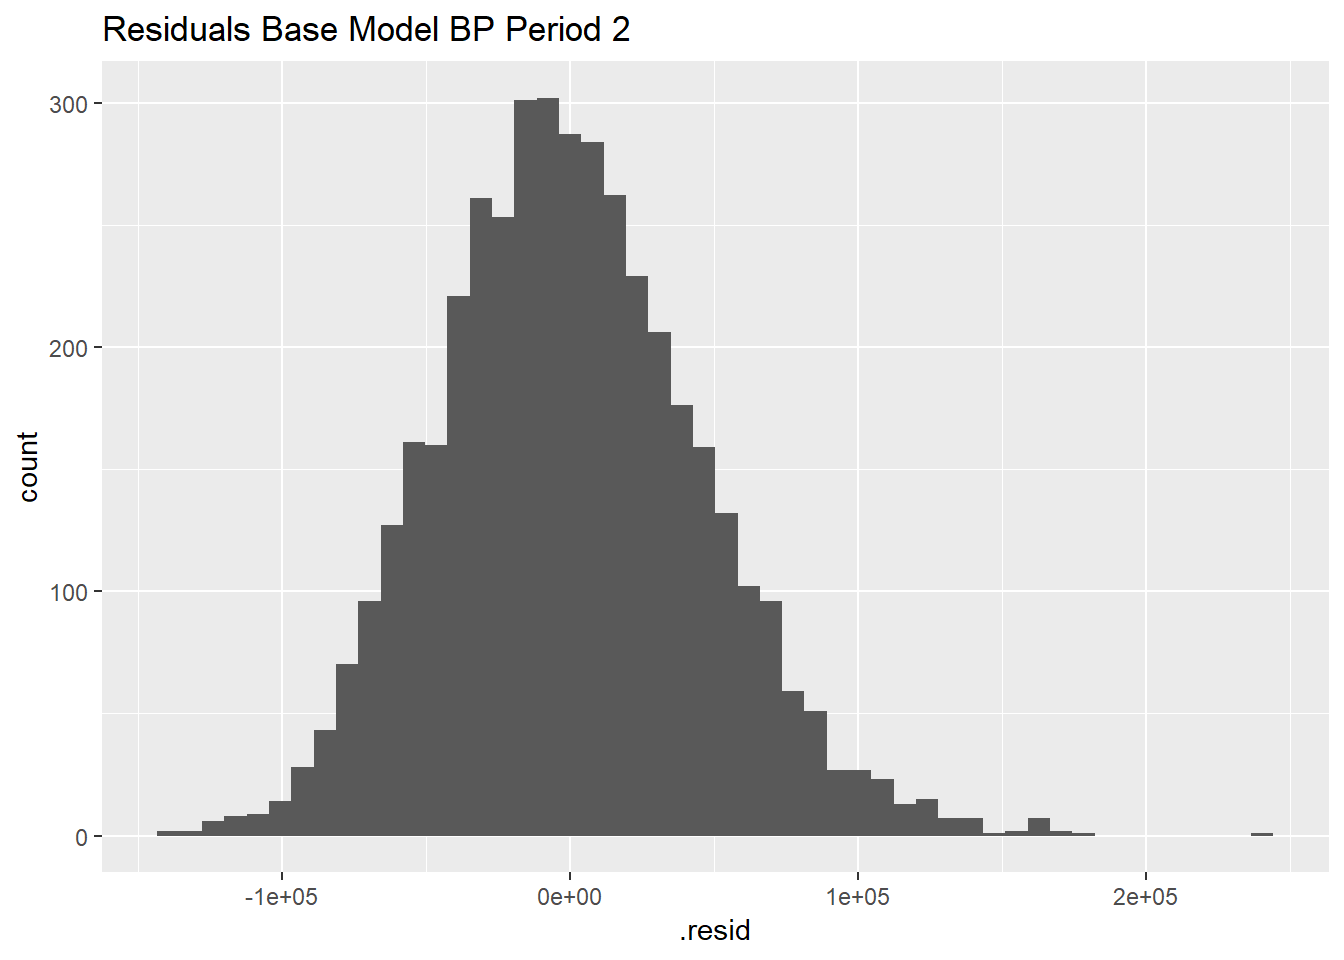
\includegraphics{bookdown-demo_files/figure-latex/unnamed-chunk-19-1.pdf}

\begin{Shaded}
\begin{Highlighting}[]
\NormalTok{bp_ols_p3_re <-}\StringTok{ }\KeywordTok{augment}\NormalTok{(bp_ols_p3, }\DataTypeTok{data =}\NormalTok{ data_bp_p3)}
\NormalTok{bp_ols_p3_re }\OperatorTok\StringTok{ }
\StringTok{  }\KeywordTok{ggplot}\NormalTok{(}\KeywordTok{aes}\NormalTok{(}\DataTypeTok{x =}\NormalTok{ .resid)) }\OperatorTok{+}
\StringTok{  }\KeywordTok{geom_histogram}\NormalTok{(}\DataTypeTok{bins =} \DecValTok{50}\NormalTok{) }\OperatorTok{+}\StringTok{ }\KeywordTok{labs}\NormalTok{(}\DataTypeTok{title =} \StringTok{"Residuals Base Model BP Period 3"}\NormalTok{)}
\end{Highlighting}
\end{Shaded}

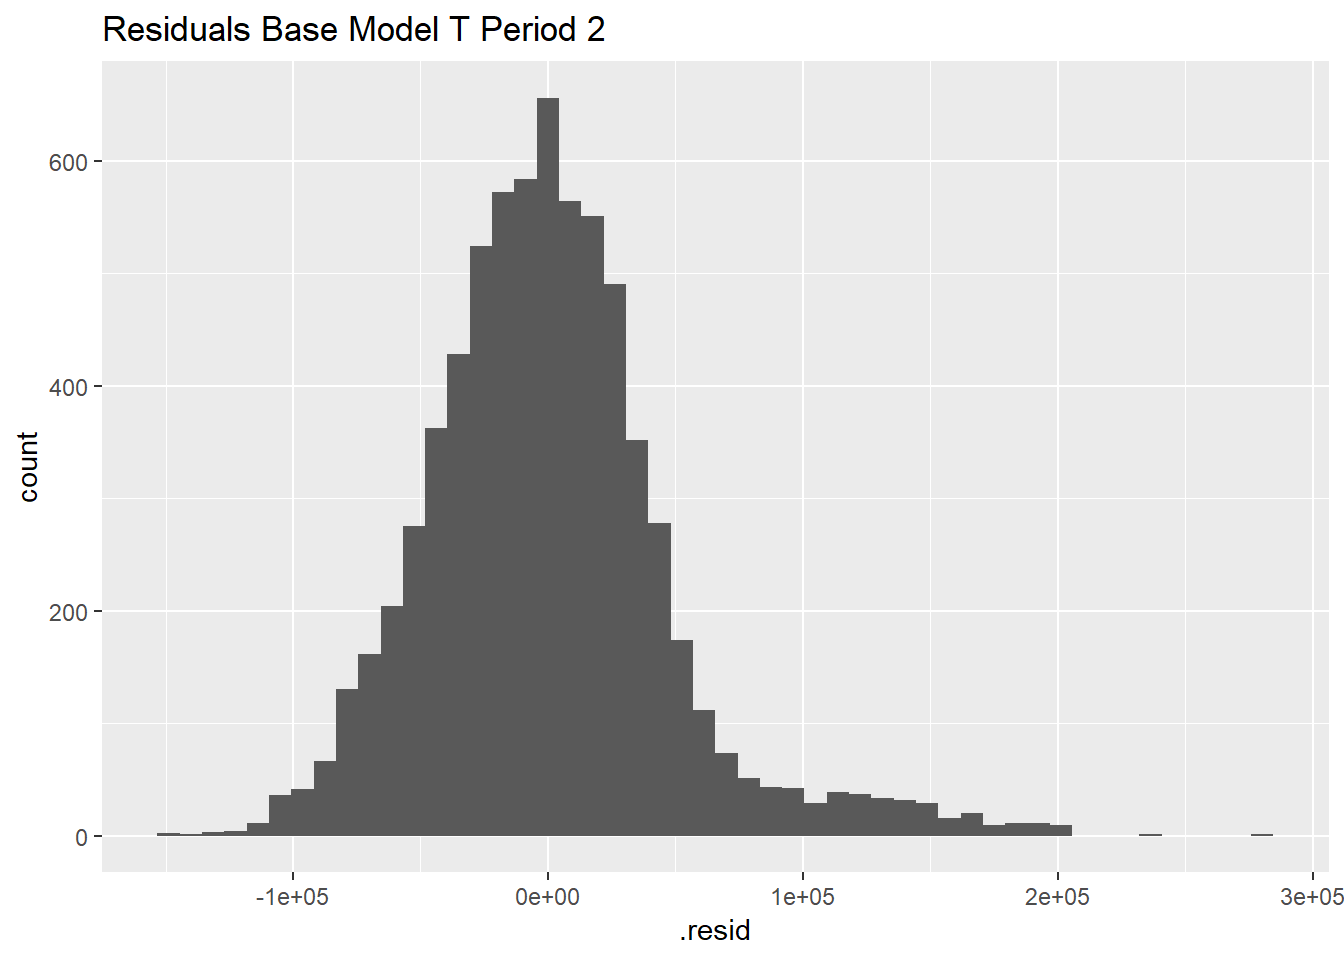
\includegraphics{bookdown-demo_files/figure-latex/unnamed-chunk-20-1.pdf}
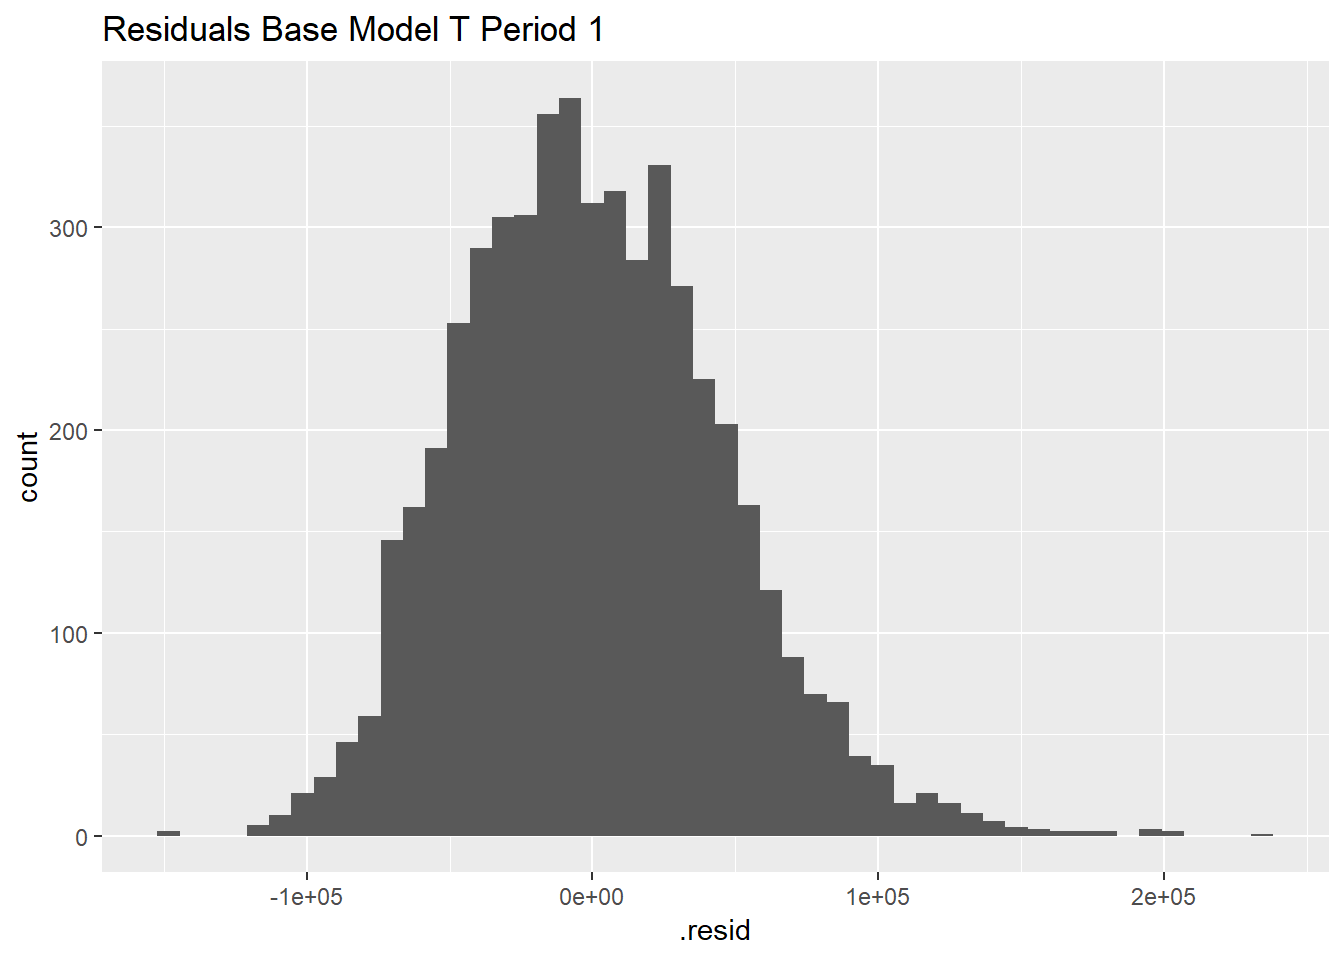
\includegraphics{bookdown-demo_files/figure-latex/unnamed-chunk-21-1.pdf}
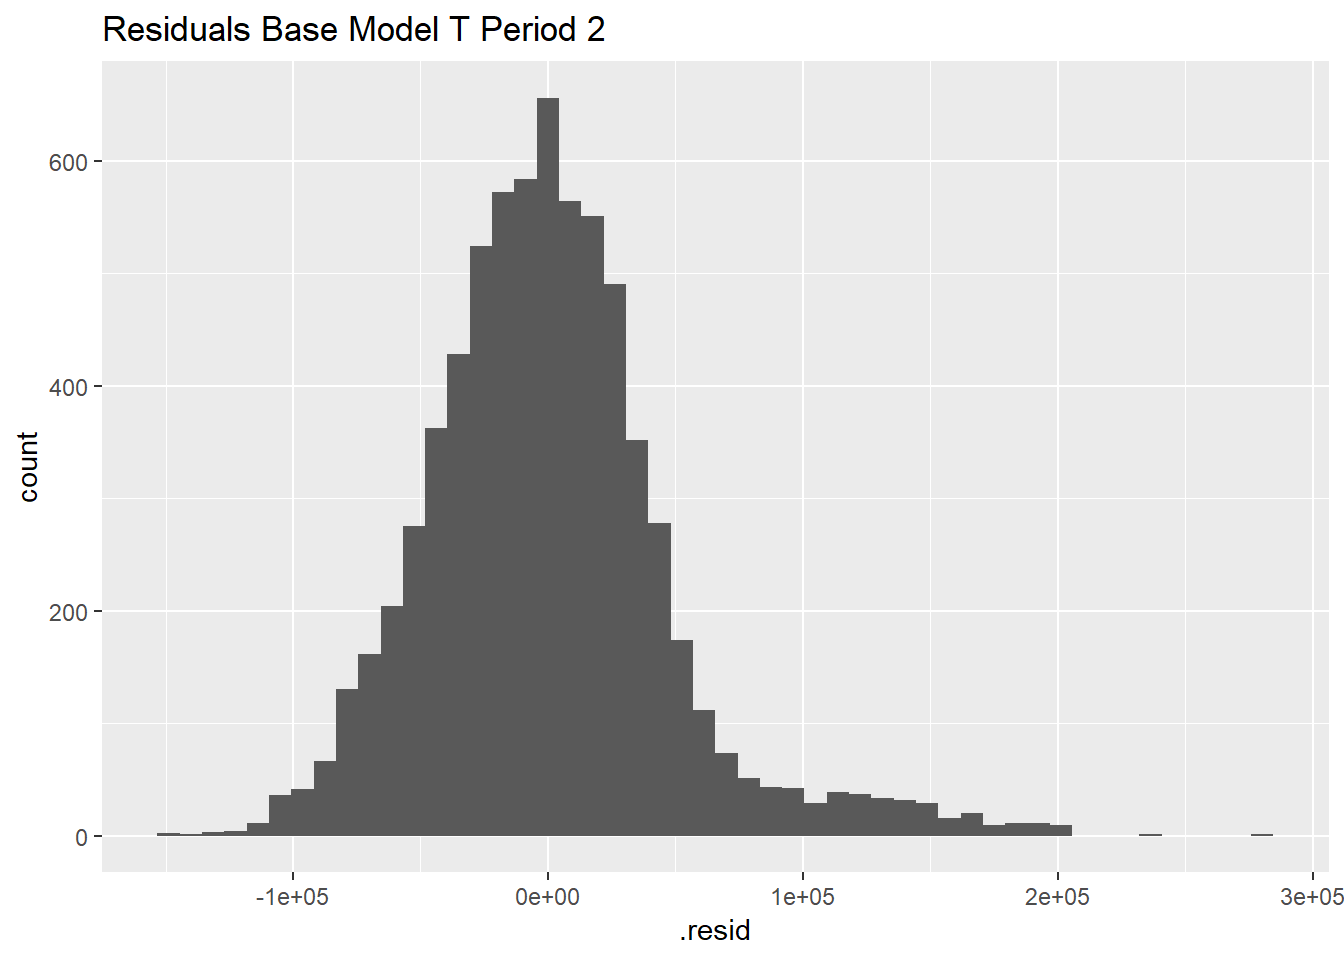
\includegraphics{bookdown-demo_files/figure-latex/unnamed-chunk-22-1.pdf}
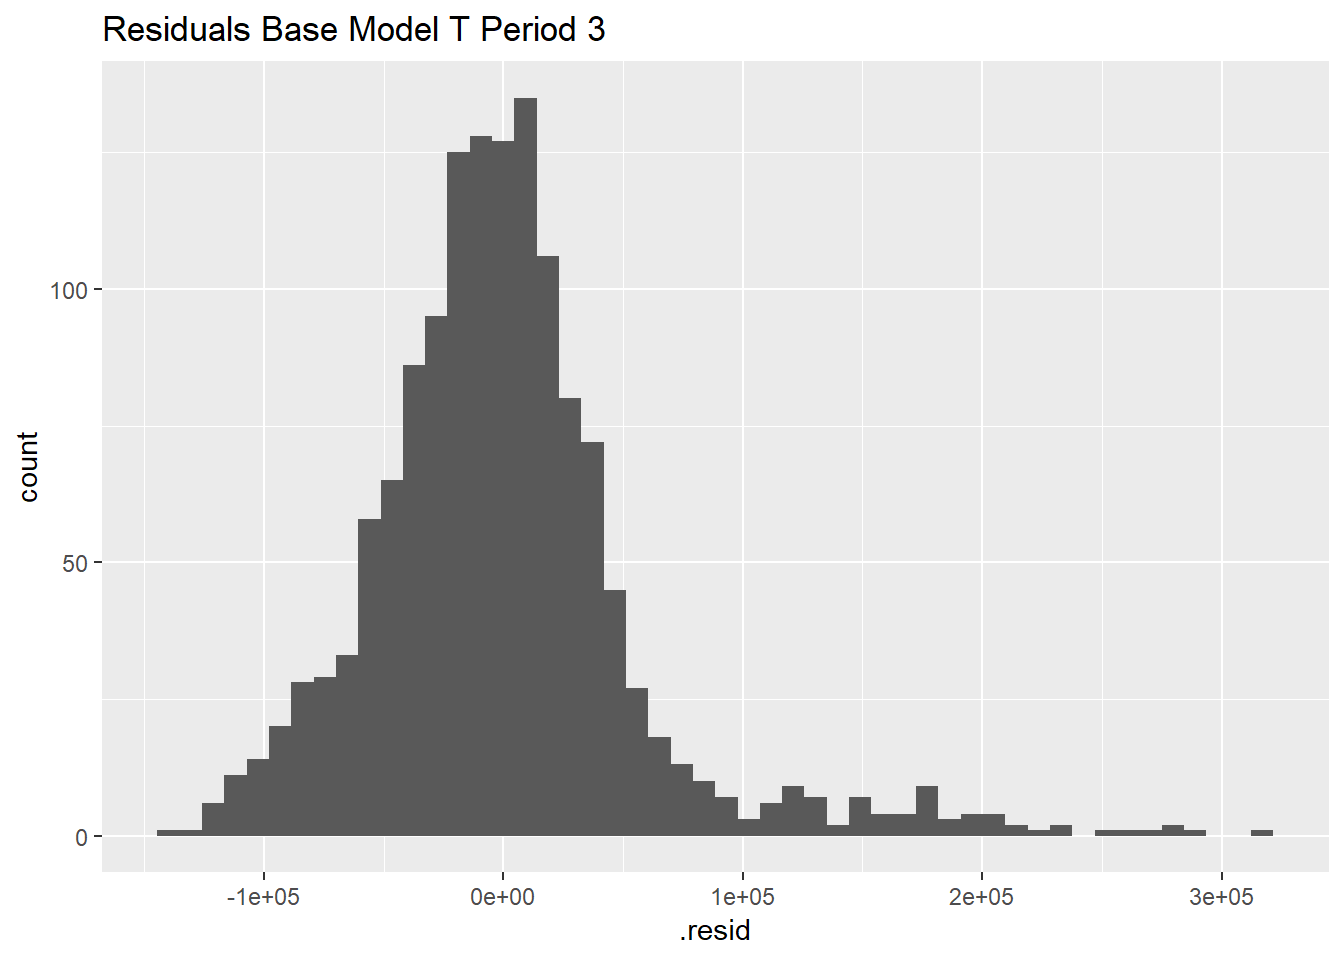
\includegraphics{bookdown-demo_files/figure-latex/unnamed-chunk-23-1.pdf}
The residuals for BP base models are close to a normal distribution. For
period 3, the is a smaller dataset available since opening of the BP
MRT, which make outliers stands out as it does not spread out as much.

\begin{Shaded}
\begin{Highlighting}[]
\NormalTok{bp_data_cont_p <-}\StringTok{ }\KeywordTok{lm}\NormalTok{(}\KeywordTok{log}\NormalTok{(resale_price) }\OperatorTok{~}\StringTok{ }\NormalTok{floor_area_sqm }\OperatorTok{+}\StringTok{ }\NormalTok{period }\OperatorTok{+}\StringTok{ }\NormalTok{connected }\OperatorTok{+}\StringTok{ }\NormalTok{near_pop_sch }\OperatorTok{+}\StringTok{ }\NormalTok{distance_towncentre }\OperatorTok{+}\StringTok{ }\NormalTok{park }\OperatorTok{+}\StringTok{ }\NormalTok{flat_type }\OperatorTok{+}\StringTok{ }\NormalTok{storey }\OperatorTok{+}\StringTok{ }\NormalTok{lease_remaining, data_bp)}

\NormalTok{tamp_data_cont_p <-}\StringTok{ }\KeywordTok{lm}\NormalTok{(}\KeywordTok{log}\NormalTok{(resale_price) }\OperatorTok{~}\StringTok{ }\NormalTok{floor_area_sqm }\OperatorTok{+}\StringTok{ }\NormalTok{period }\OperatorTok{+}\StringTok{ }\NormalTok{connected }\OperatorTok{+}\StringTok{ }\NormalTok{near_pop_sch }\OperatorTok{+}\StringTok{ }\NormalTok{distance_towncentre }\OperatorTok{+}\StringTok{ }\NormalTok{park }\OperatorTok{+}\StringTok{ }\NormalTok{flat_type }\OperatorTok{+}\StringTok{ }\NormalTok{storey }\OperatorTok{+}\StringTok{ }\NormalTok{lease_remaining, data_tamp)}

\NormalTok{bp_data_cat_p <-}\StringTok{ }\KeywordTok{lm}\NormalTok{(}\KeywordTok{log}\NormalTok{(resale_price) }\OperatorTok{~}\StringTok{ }\NormalTok{floor_area_sqm }\OperatorTok{+}\StringTok{ }\NormalTok{per }\OperatorTok{+}\StringTok{ }\NormalTok{connected }\OperatorTok{+}\StringTok{ }\NormalTok{near_pop_sch }\OperatorTok{+}\StringTok{ }\NormalTok{distance_towncentre }\OperatorTok{+}\StringTok{ }\NormalTok{park }\OperatorTok{+}\StringTok{ }\NormalTok{flat_type }\OperatorTok{+}\StringTok{ }\NormalTok{storey }\OperatorTok{+}\StringTok{ }\NormalTok{lease_remaining, data_bp)}

\NormalTok{tamp_data_cat_p <-}\StringTok{ }\KeywordTok{lm}\NormalTok{(}\KeywordTok{log}\NormalTok{(resale_price) }\OperatorTok{~}\StringTok{ }\NormalTok{floor_area_sqm }\OperatorTok{+}\StringTok{ }\NormalTok{per }\OperatorTok{+}\StringTok{ }\NormalTok{connected }\OperatorTok{+}\StringTok{ }\NormalTok{near_pop_sch }\OperatorTok{+}\StringTok{ }\NormalTok{distance_towncentre }\OperatorTok{+}\StringTok{ }\NormalTok{park }\OperatorTok{+}\StringTok{ }\NormalTok{flat_type }\OperatorTok{+}\StringTok{ }\NormalTok{storey }\OperatorTok{+}\StringTok{ }\NormalTok{lease_remaining, data_tamp)}
\end{Highlighting}
\end{Shaded}

\begin{longtable}[]{@{}lllll@{}}
\toprule
\begin{minipage}[b]{0.15\columnwidth}\raggedright\strut
\strut
\end{minipage} & \begin{minipage}[b]{0.17\columnwidth}\raggedright\strut
\strut
\end{minipage} & \begin{minipage}[b]{0.17\columnwidth}\raggedright\strut
Dependent variable:\strut
\end{minipage} & \begin{minipage}[b]{0.18\columnwidth}\raggedright\strut
\strut
\end{minipage} & \begin{minipage}[b]{0.18\columnwidth}\raggedright\strut
\strut
\end{minipage}\tabularnewline
\midrule
\endhead
\begin{minipage}[t]{0.15\columnwidth}\raggedright\strut
\strut
\end{minipage} & \begin{minipage}[t]{0.17\columnwidth}\raggedright\strut
\strut
\end{minipage} & \begin{minipage}[t]{0.17\columnwidth}\raggedright\strut
\strut
\end{minipage} & \begin{minipage}[t]{0.18\columnwidth}\raggedright\strut
\strut
\end{minipage} & \begin{minipage}[t]{0.18\columnwidth}\raggedright\strut
\strut
\end{minipage}\tabularnewline
\begin{minipage}[t]{0.15\columnwidth}\raggedright\strut
\strut
\end{minipage} & \begin{minipage}[t]{0.17\columnwidth}\raggedright\strut
\strut
\end{minipage} & \begin{minipage}[t]{0.17\columnwidth}\raggedright\strut
log(resale\_price)\strut
\end{minipage} & \begin{minipage}[t]{0.18\columnwidth}\raggedright\strut
\strut
\end{minipage} & \begin{minipage}[t]{0.18\columnwidth}\raggedright\strut
\strut
\end{minipage}\tabularnewline
\begin{minipage}[t]{0.15\columnwidth}\raggedright\strut
\strut
\end{minipage} & \begin{minipage}[t]{0.17\columnwidth}\raggedright\strut
(1) -- BP Cont\strut
\end{minipage} & \begin{minipage}[t]{0.17\columnwidth}\raggedright\strut
(2) - BP Cat\strut
\end{minipage} & \begin{minipage}[t]{0.18\columnwidth}\raggedright\strut
(3) -- T Cont\strut
\end{minipage} & \begin{minipage}[t]{0.18\columnwidth}\raggedright\strut
(4) -- T Cat\strut
\end{minipage}\tabularnewline
\begin{minipage}[t]{0.15\columnwidth}\raggedright\strut
\strut
\end{minipage} & \begin{minipage}[t]{0.17\columnwidth}\raggedright\strut
\strut
\end{minipage} & \begin{minipage}[t]{0.17\columnwidth}\raggedright\strut
\strut
\end{minipage} & \begin{minipage}[t]{0.18\columnwidth}\raggedright\strut
\strut
\end{minipage} & \begin{minipage}[t]{0.18\columnwidth}\raggedright\strut
\strut
\end{minipage}\tabularnewline
\begin{minipage}[t]{0.15\columnwidth}\raggedright\strut
floor\_area\_sqm\strut
\end{minipage} & \begin{minipage}[t]{0.17\columnwidth}\raggedright\strut
0.004***\strut
\end{minipage} & \begin{minipage}[t]{0.17\columnwidth}\raggedright\strut
0.005***\strut
\end{minipage} & \begin{minipage}[t]{0.18\columnwidth}\raggedright\strut
0.005***\strut
\end{minipage} & \begin{minipage}[t]{0.18\columnwidth}\raggedright\strut
0.006***\strut
\end{minipage}\tabularnewline
\begin{minipage}[t]{0.15\columnwidth}\raggedright\strut
\strut
\end{minipage} & \begin{minipage}[t]{0.17\columnwidth}\raggedright\strut
(0.0002)\strut
\end{minipage} & \begin{minipage}[t]{0.17\columnwidth}\raggedright\strut
(0.0002)\strut
\end{minipage} & \begin{minipage}[t]{0.18\columnwidth}\raggedright\strut
(0.0002)\strut
\end{minipage} & \begin{minipage}[t]{0.18\columnwidth}\raggedright\strut
(0.0001)\strut
\end{minipage}\tabularnewline
\begin{minipage}[t]{0.15\columnwidth}\raggedright\strut
\strut
\end{minipage} & \begin{minipage}[t]{0.17\columnwidth}\raggedright\strut
\strut
\end{minipage} & \begin{minipage}[t]{0.17\columnwidth}\raggedright\strut
\strut
\end{minipage} & \begin{minipage}[t]{0.18\columnwidth}\raggedright\strut
\strut
\end{minipage} & \begin{minipage}[t]{0.18\columnwidth}\raggedright\strut
\strut
\end{minipage}\tabularnewline
\begin{minipage}[t]{0.15\columnwidth}\raggedright\strut
period\strut
\end{minipage} & \begin{minipage}[t]{0.17\columnwidth}\raggedright\strut
0.146***\strut
\end{minipage} & \begin{minipage}[t]{0.17\columnwidth}\raggedright\strut
\strut
\end{minipage} & \begin{minipage}[t]{0.18\columnwidth}\raggedright\strut
0.143***\strut
\end{minipage} & \begin{minipage}[t]{0.18\columnwidth}\raggedright\strut
\strut
\end{minipage}\tabularnewline
\begin{minipage}[t]{0.15\columnwidth}\raggedright\strut
\strut
\end{minipage} & \begin{minipage}[t]{0.17\columnwidth}\raggedright\strut
(0.002)\strut
\end{minipage} & \begin{minipage}[t]{0.17\columnwidth}\raggedright\strut
\strut
\end{minipage} & \begin{minipage}[t]{0.18\columnwidth}\raggedright\strut
(0.002)\strut
\end{minipage} & \begin{minipage}[t]{0.18\columnwidth}\raggedright\strut
\strut
\end{minipage}\tabularnewline
\begin{minipage}[t]{0.15\columnwidth}\raggedright\strut
\strut
\end{minipage} & \begin{minipage}[t]{0.17\columnwidth}\raggedright\strut
\strut
\end{minipage} & \begin{minipage}[t]{0.17\columnwidth}\raggedright\strut
\strut
\end{minipage} & \begin{minipage}[t]{0.18\columnwidth}\raggedright\strut
\strut
\end{minipage} & \begin{minipage}[t]{0.18\columnwidth}\raggedright\strut
\strut
\end{minipage}\tabularnewline
\begin{minipage}[t]{0.15\columnwidth}\raggedright\strut
perthree\strut
\end{minipage} & \begin{minipage}[t]{0.17\columnwidth}\raggedright\strut
\strut
\end{minipage} & \begin{minipage}[t]{0.17\columnwidth}\raggedright\strut
0.216***\strut
\end{minipage} & \begin{minipage}[t]{0.18\columnwidth}\raggedright\strut
\strut
\end{minipage} & \begin{minipage}[t]{0.18\columnwidth}\raggedright\strut
0.211***\strut
\end{minipage}\tabularnewline
\begin{minipage}[t]{0.15\columnwidth}\raggedright\strut
\strut
\end{minipage} & \begin{minipage}[t]{0.17\columnwidth}\raggedright\strut
\strut
\end{minipage} & \begin{minipage}[t]{0.17\columnwidth}\raggedright\strut
(0.004)\strut
\end{minipage} & \begin{minipage}[t]{0.18\columnwidth}\raggedright\strut
\strut
\end{minipage} & \begin{minipage}[t]{0.18\columnwidth}\raggedright\strut
(0.003)\strut
\end{minipage}\tabularnewline
\begin{minipage}[t]{0.15\columnwidth}\raggedright\strut
\strut
\end{minipage} & \begin{minipage}[t]{0.17\columnwidth}\raggedright\strut
\strut
\end{minipage} & \begin{minipage}[t]{0.17\columnwidth}\raggedright\strut
\strut
\end{minipage} & \begin{minipage}[t]{0.18\columnwidth}\raggedright\strut
\strut
\end{minipage} & \begin{minipage}[t]{0.18\columnwidth}\raggedright\strut
\strut
\end{minipage}\tabularnewline
\begin{minipage}[t]{0.15\columnwidth}\raggedright\strut
pertwo\strut
\end{minipage} & \begin{minipage}[t]{0.17\columnwidth}\raggedright\strut
\strut
\end{minipage} & \begin{minipage}[t]{0.17\columnwidth}\raggedright\strut
0.235***\strut
\end{minipage} & \begin{minipage}[t]{0.18\columnwidth}\raggedright\strut
\strut
\end{minipage} & \begin{minipage}[t]{0.18\columnwidth}\raggedright\strut
0.213***\strut
\end{minipage}\tabularnewline
\begin{minipage}[t]{0.15\columnwidth}\raggedright\strut
\strut
\end{minipage} & \begin{minipage}[t]{0.17\columnwidth}\raggedright\strut
\strut
\end{minipage} & \begin{minipage}[t]{0.17\columnwidth}\raggedright\strut
(0.002)\strut
\end{minipage} & \begin{minipage}[t]{0.18\columnwidth}\raggedright\strut
\strut
\end{minipage} & \begin{minipage}[t]{0.18\columnwidth}\raggedright\strut
(0.002)\strut
\end{minipage}\tabularnewline
\begin{minipage}[t]{0.15\columnwidth}\raggedright\strut
\strut
\end{minipage} & \begin{minipage}[t]{0.17\columnwidth}\raggedright\strut
\strut
\end{minipage} & \begin{minipage}[t]{0.17\columnwidth}\raggedright\strut
\strut
\end{minipage} & \begin{minipage}[t]{0.18\columnwidth}\raggedright\strut
\strut
\end{minipage} & \begin{minipage}[t]{0.18\columnwidth}\raggedright\strut
\strut
\end{minipage}\tabularnewline
\begin{minipage}[t]{0.15\columnwidth}\raggedright\strut
connected\strut
\end{minipage} & \begin{minipage}[t]{0.17\columnwidth}\raggedright\strut
-0.037***\strut
\end{minipage} & \begin{minipage}[t]{0.17\columnwidth}\raggedright\strut
-0.042***\strut
\end{minipage} & \begin{minipage}[t]{0.18\columnwidth}\raggedright\strut
0.010***\strut
\end{minipage} & \begin{minipage}[t]{0.18\columnwidth}\raggedright\strut
0.010***\strut
\end{minipage}\tabularnewline
\begin{minipage}[t]{0.15\columnwidth}\raggedright\strut
\strut
\end{minipage} & \begin{minipage}[t]{0.17\columnwidth}\raggedright\strut
(0.005)\strut
\end{minipage} & \begin{minipage}[t]{0.17\columnwidth}\raggedright\strut
(0.004)\strut
\end{minipage} & \begin{minipage}[t]{0.18\columnwidth}\raggedright\strut
(0.003)\strut
\end{minipage} & \begin{minipage}[t]{0.18\columnwidth}\raggedright\strut
(0.003)\strut
\end{minipage}\tabularnewline
\begin{minipage}[t]{0.15\columnwidth}\raggedright\strut
\strut
\end{minipage} & \begin{minipage}[t]{0.17\columnwidth}\raggedright\strut
\strut
\end{minipage} & \begin{minipage}[t]{0.17\columnwidth}\raggedright\strut
\strut
\end{minipage} & \begin{minipage}[t]{0.18\columnwidth}\raggedright\strut
\strut
\end{minipage} & \begin{minipage}[t]{0.18\columnwidth}\raggedright\strut
\strut
\end{minipage}\tabularnewline
\begin{minipage}[t]{0.15\columnwidth}\raggedright\strut
near\_pop\_sch\strut
\end{minipage} & \begin{minipage}[t]{0.17\columnwidth}\raggedright\strut
\strut
\end{minipage} & \begin{minipage}[t]{0.17\columnwidth}\raggedright\strut
\strut
\end{minipage} & \begin{minipage}[t]{0.18\columnwidth}\raggedright\strut
0.005**\strut
\end{minipage} & \begin{minipage}[t]{0.18\columnwidth}\raggedright\strut
0.004**\strut
\end{minipage}\tabularnewline
\begin{minipage}[t]{0.15\columnwidth}\raggedright\strut
\strut
\end{minipage} & \begin{minipage}[t]{0.17\columnwidth}\raggedright\strut
\strut
\end{minipage} & \begin{minipage}[t]{0.17\columnwidth}\raggedright\strut
\strut
\end{minipage} & \begin{minipage}[t]{0.18\columnwidth}\raggedright\strut
(0.002)\strut
\end{minipage} & \begin{minipage}[t]{0.18\columnwidth}\raggedright\strut
(0.002)\strut
\end{minipage}\tabularnewline
\begin{minipage}[t]{0.15\columnwidth}\raggedright\strut
\strut
\end{minipage} & \begin{minipage}[t]{0.17\columnwidth}\raggedright\strut
\strut
\end{minipage} & \begin{minipage}[t]{0.17\columnwidth}\raggedright\strut
\strut
\end{minipage} & \begin{minipage}[t]{0.18\columnwidth}\raggedright\strut
\strut
\end{minipage} & \begin{minipage}[t]{0.18\columnwidth}\raggedright\strut
\strut
\end{minipage}\tabularnewline
\begin{minipage}[t]{0.15\columnwidth}\raggedright\strut
distance\_towncentre\strut
\end{minipage} & \begin{minipage}[t]{0.17\columnwidth}\raggedright\strut
-0.187***\strut
\end{minipage} & \begin{minipage}[t]{0.17\columnwidth}\raggedright\strut
-0.193***\strut
\end{minipage} & \begin{minipage}[t]{0.18\columnwidth}\raggedright\strut
-0.099***\strut
\end{minipage} & \begin{minipage}[t]{0.18\columnwidth}\raggedright\strut
-0.098***\strut
\end{minipage}\tabularnewline
\begin{minipage}[t]{0.15\columnwidth}\raggedright\strut
\strut
\end{minipage} & \begin{minipage}[t]{0.17\columnwidth}\raggedright\strut
(0.006)\strut
\end{minipage} & \begin{minipage}[t]{0.17\columnwidth}\raggedright\strut
(0.005)\strut
\end{minipage} & \begin{minipage}[t]{0.18\columnwidth}\raggedright\strut
(0.002)\strut
\end{minipage} & \begin{minipage}[t]{0.18\columnwidth}\raggedright\strut
(0.002)\strut
\end{minipage}\tabularnewline
\begin{minipage}[t]{0.15\columnwidth}\raggedright\strut
\strut
\end{minipage} & \begin{minipage}[t]{0.17\columnwidth}\raggedright\strut
\strut
\end{minipage} & \begin{minipage}[t]{0.17\columnwidth}\raggedright\strut
\strut
\end{minipage} & \begin{minipage}[t]{0.18\columnwidth}\raggedright\strut
\strut
\end{minipage} & \begin{minipage}[t]{0.18\columnwidth}\raggedright\strut
\strut
\end{minipage}\tabularnewline
\begin{minipage}[t]{0.15\columnwidth}\raggedright\strut
park\strut
\end{minipage} & \begin{minipage}[t]{0.17\columnwidth}\raggedright\strut
-0.004\strut
\end{minipage} & \begin{minipage}[t]{0.17\columnwidth}\raggedright\strut
-0.009\strut
\end{minipage} & \begin{minipage}[t]{0.18\columnwidth}\raggedright\strut
0.001\strut
\end{minipage} & \begin{minipage}[t]{0.18\columnwidth}\raggedright\strut
0.005\strut
\end{minipage}\tabularnewline
\begin{minipage}[t]{0.15\columnwidth}\raggedright\strut
\strut
\end{minipage} & \begin{minipage}[t]{0.17\columnwidth}\raggedright\strut
(0.006)\strut
\end{minipage} & \begin{minipage}[t]{0.17\columnwidth}\raggedright\strut
(0.006)\strut
\end{minipage} & \begin{minipage}[t]{0.18\columnwidth}\raggedright\strut
(0.004)\strut
\end{minipage} & \begin{minipage}[t]{0.18\columnwidth}\raggedright\strut
(0.004)\strut
\end{minipage}\tabularnewline
\begin{minipage}[t]{0.15\columnwidth}\raggedright\strut
\strut
\end{minipage} & \begin{minipage}[t]{0.17\columnwidth}\raggedright\strut
\strut
\end{minipage} & \begin{minipage}[t]{0.17\columnwidth}\raggedright\strut
\strut
\end{minipage} & \begin{minipage}[t]{0.18\columnwidth}\raggedright\strut
\strut
\end{minipage} & \begin{minipage}[t]{0.18\columnwidth}\raggedright\strut
\strut
\end{minipage}\tabularnewline
\begin{minipage}[t]{0.15\columnwidth}\raggedright\strut
flat\_type3 ROOM\strut
\end{minipage} & \begin{minipage}[t]{0.17\columnwidth}\raggedright\strut
0.485***\strut
\end{minipage} & \begin{minipage}[t]{0.17\columnwidth}\raggedright\strut
0.375***\strut
\end{minipage} & \begin{minipage}[t]{0.18\columnwidth}\raggedright\strut
0.286***\strut
\end{minipage} & \begin{minipage}[t]{0.18\columnwidth}\raggedright\strut
0.206***\strut
\end{minipage}\tabularnewline
\begin{minipage}[t]{0.15\columnwidth}\raggedright\strut
\strut
\end{minipage} & \begin{minipage}[t]{0.17\columnwidth}\raggedright\strut
(0.040)\strut
\end{minipage} & \begin{minipage}[t]{0.17\columnwidth}\raggedright\strut
(0.034)\strut
\end{minipage} & \begin{minipage}[t]{0.18\columnwidth}\raggedright\strut
(0.026)\strut
\end{minipage} & \begin{minipage}[t]{0.18\columnwidth}\raggedright\strut
(0.023)\strut
\end{minipage}\tabularnewline
\begin{minipage}[t]{0.15\columnwidth}\raggedright\strut
\strut
\end{minipage} & \begin{minipage}[t]{0.17\columnwidth}\raggedright\strut
\strut
\end{minipage} & \begin{minipage}[t]{0.17\columnwidth}\raggedright\strut
\strut
\end{minipage} & \begin{minipage}[t]{0.18\columnwidth}\raggedright\strut
\strut
\end{minipage} & \begin{minipage}[t]{0.18\columnwidth}\raggedright\strut
\strut
\end{minipage}\tabularnewline
\begin{minipage}[t]{0.15\columnwidth}\raggedright\strut
flat\_type4 ROOM\strut
\end{minipage} & \begin{minipage}[t]{0.17\columnwidth}\raggedright\strut
0.545***\strut
\end{minipage} & \begin{minipage}[t]{0.17\columnwidth}\raggedright\strut
0.427***\strut
\end{minipage} & \begin{minipage}[t]{0.18\columnwidth}\raggedright\strut
0.363***\strut
\end{minipage} & \begin{minipage}[t]{0.18\columnwidth}\raggedright\strut
0.279***\strut
\end{minipage}\tabularnewline
\begin{minipage}[t]{0.15\columnwidth}\raggedright\strut
\strut
\end{minipage} & \begin{minipage}[t]{0.17\columnwidth}\raggedright\strut
(0.041)\strut
\end{minipage} & \begin{minipage}[t]{0.17\columnwidth}\raggedright\strut
(0.035)\strut
\end{minipage} & \begin{minipage}[t]{0.18\columnwidth}\raggedright\strut
(0.026)\strut
\end{minipage} & \begin{minipage}[t]{0.18\columnwidth}\raggedright\strut
(0.023)\strut
\end{minipage}\tabularnewline
\begin{minipage}[t]{0.15\columnwidth}\raggedright\strut
\strut
\end{minipage} & \begin{minipage}[t]{0.17\columnwidth}\raggedright\strut
\strut
\end{minipage} & \begin{minipage}[t]{0.17\columnwidth}\raggedright\strut
\strut
\end{minipage} & \begin{minipage}[t]{0.18\columnwidth}\raggedright\strut
\strut
\end{minipage} & \begin{minipage}[t]{0.18\columnwidth}\raggedright\strut
\strut
\end{minipage}\tabularnewline
\begin{minipage}[t]{0.15\columnwidth}\raggedright\strut
flat\_type5 ROOM\strut
\end{minipage} & \begin{minipage}[t]{0.17\columnwidth}\raggedright\strut
0.633***\strut
\end{minipage} & \begin{minipage}[t]{0.17\columnwidth}\raggedright\strut
0.515***\strut
\end{minipage} & \begin{minipage}[t]{0.18\columnwidth}\raggedright\strut
0.408***\strut
\end{minipage} & \begin{minipage}[t]{0.18\columnwidth}\raggedright\strut
0.320***\strut
\end{minipage}\tabularnewline
\begin{minipage}[t]{0.15\columnwidth}\raggedright\strut
\strut
\end{minipage} & \begin{minipage}[t]{0.17\columnwidth}\raggedright\strut
(0.042)\strut
\end{minipage} & \begin{minipage}[t]{0.17\columnwidth}\raggedright\strut
(0.036)\strut
\end{minipage} & \begin{minipage}[t]{0.18\columnwidth}\raggedright\strut
(0.028)\strut
\end{minipage} & \begin{minipage}[t]{0.18\columnwidth}\raggedright\strut
(0.024)\strut
\end{minipage}\tabularnewline
\begin{minipage}[t]{0.15\columnwidth}\raggedright\strut
\strut
\end{minipage} & \begin{minipage}[t]{0.17\columnwidth}\raggedright\strut
\strut
\end{minipage} & \begin{minipage}[t]{0.17\columnwidth}\raggedright\strut
\strut
\end{minipage} & \begin{minipage}[t]{0.18\columnwidth}\raggedright\strut
\strut
\end{minipage} & \begin{minipage}[t]{0.18\columnwidth}\raggedright\strut
\strut
\end{minipage}\tabularnewline
\begin{minipage}[t]{0.15\columnwidth}\raggedright\strut
flat\_typeEXECUTIVE\strut
\end{minipage} & \begin{minipage}[t]{0.17\columnwidth}\raggedright\strut
0.767***\strut
\end{minipage} & \begin{minipage}[t]{0.17\columnwidth}\raggedright\strut
0.643***\strut
\end{minipage} & \begin{minipage}[t]{0.18\columnwidth}\raggedright\strut
0.512***\strut
\end{minipage} & \begin{minipage}[t]{0.18\columnwidth}\raggedright\strut
0.427***\strut
\end{minipage}\tabularnewline
\begin{minipage}[t]{0.15\columnwidth}\raggedright\strut
\strut
\end{minipage} & \begin{minipage}[t]{0.17\columnwidth}\raggedright\strut
(0.044)\strut
\end{minipage} & \begin{minipage}[t]{0.17\columnwidth}\raggedright\strut
(0.038)\strut
\end{minipage} & \begin{minipage}[t]{0.18\columnwidth}\raggedright\strut
(0.029)\strut
\end{minipage} & \begin{minipage}[t]{0.18\columnwidth}\raggedright\strut
(0.026)\strut
\end{minipage}\tabularnewline
\begin{minipage}[t]{0.15\columnwidth}\raggedright\strut
\strut
\end{minipage} & \begin{minipage}[t]{0.17\columnwidth}\raggedright\strut
\strut
\end{minipage} & \begin{minipage}[t]{0.17\columnwidth}\raggedright\strut
\strut
\end{minipage} & \begin{minipage}[t]{0.18\columnwidth}\raggedright\strut
\strut
\end{minipage} & \begin{minipage}[t]{0.18\columnwidth}\raggedright\strut
\strut
\end{minipage}\tabularnewline
\begin{minipage}[t]{0.15\columnwidth}\raggedright\strut
flat\_typeMULTI-GENERATION\strut
\end{minipage} & \begin{minipage}[t]{0.17\columnwidth}\raggedright\strut
\strut
\end{minipage} & \begin{minipage}[t]{0.17\columnwidth}\raggedright\strut
\strut
\end{minipage} & \begin{minipage}[t]{0.18\columnwidth}\raggedright\strut
0.649***\strut
\end{minipage} & \begin{minipage}[t]{0.18\columnwidth}\raggedright\strut
0.586***\strut
\end{minipage}\tabularnewline
\begin{minipage}[t]{0.15\columnwidth}\raggedright\strut
\strut
\end{minipage} & \begin{minipage}[t]{0.17\columnwidth}\raggedright\strut
\strut
\end{minipage} & \begin{minipage}[t]{0.17\columnwidth}\raggedright\strut
\strut
\end{minipage} & \begin{minipage}[t]{0.18\columnwidth}\raggedright\strut
(0.039)\strut
\end{minipage} & \begin{minipage}[t]{0.18\columnwidth}\raggedright\strut
(0.034)\strut
\end{minipage}\tabularnewline
\begin{minipage}[t]{0.15\columnwidth}\raggedright\strut
\strut
\end{minipage} & \begin{minipage}[t]{0.17\columnwidth}\raggedright\strut
\strut
\end{minipage} & \begin{minipage}[t]{0.17\columnwidth}\raggedright\strut
\strut
\end{minipage} & \begin{minipage}[t]{0.18\columnwidth}\raggedright\strut
\strut
\end{minipage} & \begin{minipage}[t]{0.18\columnwidth}\raggedright\strut
\strut
\end{minipage}\tabularnewline
\begin{minipage}[t]{0.15\columnwidth}\raggedright\strut
storey\strut
\end{minipage} & \begin{minipage}[t]{0.17\columnwidth}\raggedright\strut
0.007***\strut
\end{minipage} & \begin{minipage}[t]{0.17\columnwidth}\raggedright\strut
0.007***\strut
\end{minipage} & \begin{minipage}[t]{0.18\columnwidth}\raggedright\strut
0.007***\strut
\end{minipage} & \begin{minipage}[t]{0.18\columnwidth}\raggedright\strut
0.007***\strut
\end{minipage}\tabularnewline
\begin{minipage}[t]{0.15\columnwidth}\raggedright\strut
\strut
\end{minipage} & \begin{minipage}[t]{0.17\columnwidth}\raggedright\strut
(0.0002)\strut
\end{minipage} & \begin{minipage}[t]{0.17\columnwidth}\raggedright\strut
(0.0002)\strut
\end{minipage} & \begin{minipage}[t]{0.18\columnwidth}\raggedright\strut
(0.0003)\strut
\end{minipage} & \begin{minipage}[t]{0.18\columnwidth}\raggedright\strut
(0.0002)\strut
\end{minipage}\tabularnewline
\begin{minipage}[t]{0.15\columnwidth}\raggedright\strut
\strut
\end{minipage} & \begin{minipage}[t]{0.17\columnwidth}\raggedright\strut
\strut
\end{minipage} & \begin{minipage}[t]{0.17\columnwidth}\raggedright\strut
\strut
\end{minipage} & \begin{minipage}[t]{0.18\columnwidth}\raggedright\strut
\strut
\end{minipage} & \begin{minipage}[t]{0.18\columnwidth}\raggedright\strut
\strut
\end{minipage}\tabularnewline
\begin{minipage}[t]{0.15\columnwidth}\raggedright\strut
lease\_remaining\strut
\end{minipage} & \begin{minipage}[t]{0.17\columnwidth}\raggedright\strut
0.008***\strut
\end{minipage} & \begin{minipage}[t]{0.17\columnwidth}\raggedright\strut
0.009***\strut
\end{minipage} & \begin{minipage}[t]{0.18\columnwidth}\raggedright\strut
0.005***\strut
\end{minipage} & \begin{minipage}[t]{0.18\columnwidth}\raggedright\strut
0.005***\strut
\end{minipage}\tabularnewline
\begin{minipage}[t]{0.15\columnwidth}\raggedright\strut
\strut
\end{minipage} & \begin{minipage}[t]{0.17\columnwidth}\raggedright\strut
(0.0003)\strut
\end{minipage} & \begin{minipage}[t]{0.17\columnwidth}\raggedright\strut
(0.0002)\strut
\end{minipage} & \begin{minipage}[t]{0.18\columnwidth}\raggedright\strut
(0.0002)\strut
\end{minipage} & \begin{minipage}[t]{0.18\columnwidth}\raggedright\strut
(0.0002)\strut
\end{minipage}\tabularnewline
\begin{minipage}[t]{0.15\columnwidth}\raggedright\strut
\strut
\end{minipage} & \begin{minipage}[t]{0.17\columnwidth}\raggedright\strut
\strut
\end{minipage} & \begin{minipage}[t]{0.17\columnwidth}\raggedright\strut
\strut
\end{minipage} & \begin{minipage}[t]{0.18\columnwidth}\raggedright\strut
\strut
\end{minipage} & \begin{minipage}[t]{0.18\columnwidth}\raggedright\strut
\strut
\end{minipage}\tabularnewline
\begin{minipage}[t]{0.15\columnwidth}\raggedright\strut
Constant\strut
\end{minipage} & \begin{minipage}[t]{0.17\columnwidth}\raggedright\strut
11.058***\strut
\end{minipage} & \begin{minipage}[t]{0.17\columnwidth}\raggedright\strut
11.206***\strut
\end{minipage} & \begin{minipage}[t]{0.18\columnwidth}\raggedright\strut
11.452***\strut
\end{minipage} & \begin{minipage}[t]{0.18\columnwidth}\raggedright\strut
11.623***\strut
\end{minipage}\tabularnewline
\begin{minipage}[t]{0.15\columnwidth}\raggedright\strut
\strut
\end{minipage} & \begin{minipage}[t]{0.17\columnwidth}\raggedright\strut
(0.053)\strut
\end{minipage} & \begin{minipage}[t]{0.17\columnwidth}\raggedright\strut
(0.044)\strut
\end{minipage} & \begin{minipage}[t]{0.18\columnwidth}\raggedright\strut
(0.033)\strut
\end{minipage} & \begin{minipage}[t]{0.18\columnwidth}\raggedright\strut
(0.029)\strut
\end{minipage}\tabularnewline
\begin{minipage}[t]{0.15\columnwidth}\raggedright\strut
\strut
\end{minipage} & \begin{minipage}[t]{0.17\columnwidth}\raggedright\strut
\strut
\end{minipage} & \begin{minipage}[t]{0.17\columnwidth}\raggedright\strut
\strut
\end{minipage} & \begin{minipage}[t]{0.18\columnwidth}\raggedright\strut
\strut
\end{minipage} & \begin{minipage}[t]{0.18\columnwidth}\raggedright\strut
\strut
\end{minipage}\tabularnewline
\begin{minipage}[t]{0.15\columnwidth}\raggedright\strut
\strut
\end{minipage} & \begin{minipage}[t]{0.17\columnwidth}\raggedright\strut
\strut
\end{minipage} & \begin{minipage}[t]{0.17\columnwidth}\raggedright\strut
\strut
\end{minipage} & \begin{minipage}[t]{0.18\columnwidth}\raggedright\strut
\strut
\end{minipage} & \begin{minipage}[t]{0.18\columnwidth}\raggedright\strut
\strut
\end{minipage}\tabularnewline
\begin{minipage}[t]{0.15\columnwidth}\raggedright\strut
Observations\strut
\end{minipage} & \begin{minipage}[t]{0.17\columnwidth}\raggedright\strut
7,897\strut
\end{minipage} & \begin{minipage}[t]{0.17\columnwidth}\raggedright\strut
7,897\strut
\end{minipage} & \begin{minipage}[t]{0.18\columnwidth}\raggedright\strut
13,642\strut
\end{minipage} & \begin{minipage}[t]{0.18\columnwidth}\raggedright\strut
13,642\strut
\end{minipage}\tabularnewline
\begin{minipage}[t]{0.15\columnwidth}\raggedright\strut
R2\strut
\end{minipage} & \begin{minipage}[t]{0.17\columnwidth}\raggedright\strut
0.788\strut
\end{minipage} & \begin{minipage}[t]{0.17\columnwidth}\raggedright\strut
0.845\strut
\end{minipage} & \begin{minipage}[t]{0.18\columnwidth}\raggedright\strut
0.831\strut
\end{minipage} & \begin{minipage}[t]{0.18\columnwidth}\raggedright\strut
0.868\strut
\end{minipage}\tabularnewline
\begin{minipage}[t]{0.15\columnwidth}\raggedright\strut
Adjusted R2\strut
\end{minipage} & \begin{minipage}[t]{0.17\columnwidth}\raggedright\strut
0.788\strut
\end{minipage} & \begin{minipage}[t]{0.17\columnwidth}\raggedright\strut
0.845\strut
\end{minipage} & \begin{minipage}[t]{0.18\columnwidth}\raggedright\strut
0.831\strut
\end{minipage} & \begin{minipage}[t]{0.18\columnwidth}\raggedright\strut
0.868\strut
\end{minipage}\tabularnewline
\begin{minipage}[t]{0.15\columnwidth}\raggedright\strut
Residual Std. Error\strut
\end{minipage} & \begin{minipage}[t]{0.17\columnwidth}\raggedright\strut
0.111 (df = 7885)\strut
\end{minipage} & \begin{minipage}[t]{0.17\columnwidth}\raggedright\strut
0.095 (df = 7884)\strut
\end{minipage} & \begin{minipage}[t]{0.18\columnwidth}\raggedright\strut
0.102 (df = 13628)\strut
\end{minipage} & \begin{minipage}[t]{0.18\columnwidth}\raggedright\strut
0.090 (df = 13627)\strut
\end{minipage}\tabularnewline
\begin{minipage}[t]{0.15\columnwidth}\raggedright\strut
F Statistic\strut
\end{minipage} & \begin{minipage}[t]{0.17\columnwidth}\raggedright\strut
2,666.485*** (df = 11; 7885)\strut
\end{minipage} & \begin{minipage}[t]{0.17\columnwidth}\raggedright\strut
3,574.714*** (df = 12; 7884)\strut
\end{minipage} & \begin{minipage}[t]{0.18\columnwidth}\raggedright\strut
5,165.174*** (df = 13; 13628)\strut
\end{minipage} & \begin{minipage}[t]{0.18\columnwidth}\raggedright\strut
6,414.803*** (df = 14; 13627)\strut
\end{minipage}\tabularnewline
\bottomrule
\end{longtable}

Note: *p\textless{}0.1; **p\textless{}0.05; ***p\textless{}0.01

The log-linear regression provides us the coefficients with the
percentage change of the variable with respect to resale price. Hence,
connected to MRT station for Bukit Panjang

\chapter{Method 2 - Clustering}\label{method-2---clustering}

For Tampines Town, clustering is performed using factor analysis and k
means. The street names are shortened for easier interpretation on the
graphs. I summarised the continuous variables for by the taking the mean
of 1. Resale price 2. Lease remaining 3. Distance to mrt 4. Floor square
area

The clusters are done separately for each period for comparison. The
factor loadings of each period as follows:

\begin{Shaded}
\begin{Highlighting}[]
\NormalTok{tamp_block <-}\StringTok{ }\NormalTok{data_tamp }\OperatorTok
\StringTok{  }\KeywordTok{group_by}\NormalTok{(short_street_name,period) }\OperatorTok\StringTok{ }
\StringTok{  }\KeywordTok{summarise}\NormalTok{(}\DataTypeTok{mean_price =} \KeywordTok{mean}\NormalTok{(resale_price)}\OperatorTok{/}\DecValTok{1000}\NormalTok{, }\DataTypeTok{mean_distance_mrt =} \KeywordTok{mean}\NormalTok{(distance_mrt),}\DataTypeTok{mean_lease_remaining =} \KeywordTok{mean}\NormalTok{(lease_remaining),}\DataTypeTok{mean_floor_square =} \KeywordTok{mean}\NormalTok{(floor_area_sqm))}
\end{Highlighting}
\end{Shaded}

\begin{Shaded}
\begin{Highlighting}[]
\NormalTok{tamp_block_p1 <-}\StringTok{ }\NormalTok{tamp_block }\OperatorTok\StringTok{ }
\StringTok{  }\KeywordTok{filter}\NormalTok{(period }\OperatorTok{==}\StringTok{ }\DecValTok{1}\NormalTok{)}

\NormalTok{tamp_block_p2 <-}\StringTok{ }\NormalTok{tamp_block }\OperatorTok\StringTok{ }
\StringTok{  }\KeywordTok{filter}\NormalTok{(period }\OperatorTok{==}\StringTok{ }\DecValTok{2}\NormalTok{)}

\NormalTok{tamp_block_p3 <-}\StringTok{ }\NormalTok{tamp_block }\OperatorTok\StringTok{ }
\StringTok{  }\KeywordTok{filter}\NormalTok{(period }\OperatorTok{==}\StringTok{ }\DecValTok{3}\NormalTok{)}
\end{Highlighting}
\end{Shaded}

\begin{Shaded}
\begin{Highlighting}[]
\NormalTok{fa_s <-}\StringTok{ }\NormalTok{tamp_block_p1 }\OperatorTok\StringTok{ }
\StringTok{  }\KeywordTok{column_to_rownames}\NormalTok{(}\DataTypeTok{var =} \StringTok{"short_street_name"}\NormalTok{) }\OperatorTok\StringTok{ }
\StringTok{  }\KeywordTok{select}\NormalTok{(}\OperatorTok{-}\NormalTok{period) }\OperatorTok\StringTok{ }
\StringTok{  }\KeywordTok{principal}\NormalTok{(}\DataTypeTok{nfactors =} \DecValTok{4}\NormalTok{, }\DataTypeTok{rotate =} \StringTok{"varimax"}\NormalTok{)}
\end{Highlighting}
\end{Shaded}

\begin{Shaded}
\begin{Highlighting}[]
\NormalTok{fa1l<-fa_s[[}\StringTok{'loadings'}\NormalTok{]] }\OperatorTok\StringTok{ }
\StringTok{  }\KeywordTok{unclass}\NormalTok{() }\OperatorTok\StringTok{ }
\StringTok{  }\KeywordTok{as_tibble}\NormalTok{(}\DataTypeTok{rownames =} \StringTok{"short_street_name"}\NormalTok{) }\OperatorTok\StringTok{  }\CommentTok{# convert loadings to a tibble or easy plotting }
\StringTok{  }\KeywordTok{gather}\NormalTok{(}\DataTypeTok{key =} \StringTok{"component"}\NormalTok{, }\DataTypeTok{value =} \StringTok{"value"}\NormalTok{, }\OperatorTok{-}\NormalTok{short_street_name) }\OperatorTok\StringTok{ }
\StringTok{  }\KeywordTok{ggplot}\NormalTok{(}\KeywordTok{aes}\NormalTok{(}\DataTypeTok{x =}\NormalTok{ short_street_name, }\DataTypeTok{y =}\NormalTok{ value)) }\OperatorTok{+}\StringTok{ }
\StringTok{  }\KeywordTok{geom_hline}\NormalTok{(}\DataTypeTok{yintercept =} \DecValTok{0}\NormalTok{) }\OperatorTok{+}\StringTok{ }
\StringTok{  }\KeywordTok{geom_point}\NormalTok{() }\OperatorTok{+}
\StringTok{  }\KeywordTok{coord_flip}\NormalTok{() }\OperatorTok{+}
\StringTok{  }\KeywordTok{facet_grid}\NormalTok{(}\OperatorTok{~}\NormalTok{component)}
\end{Highlighting}
\end{Shaded}

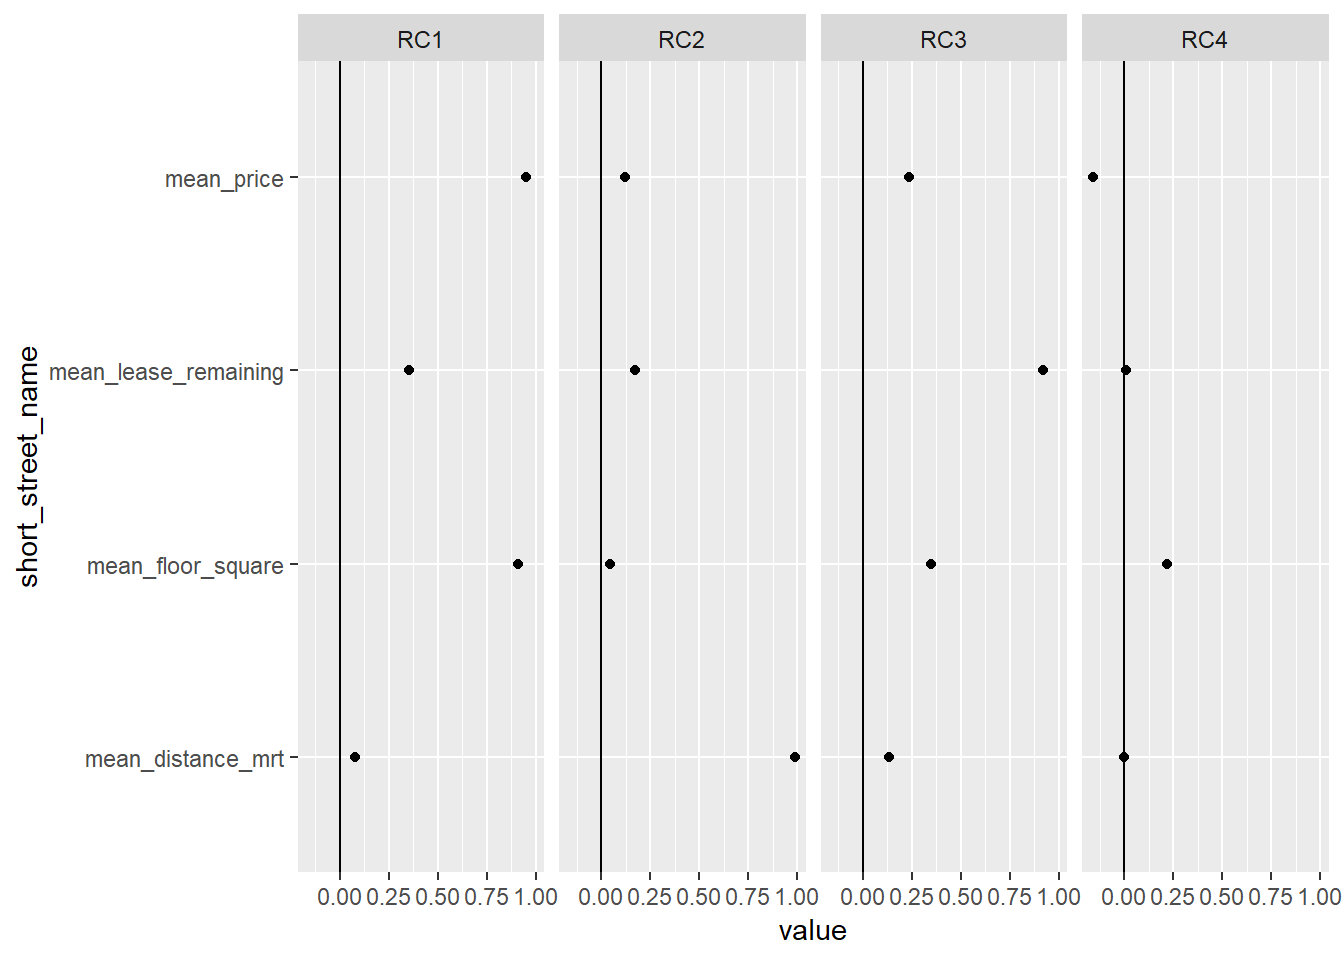
\includegraphics{bookdown-demo_files/figure-latex/unnamed-chunk-39-1.pdf}
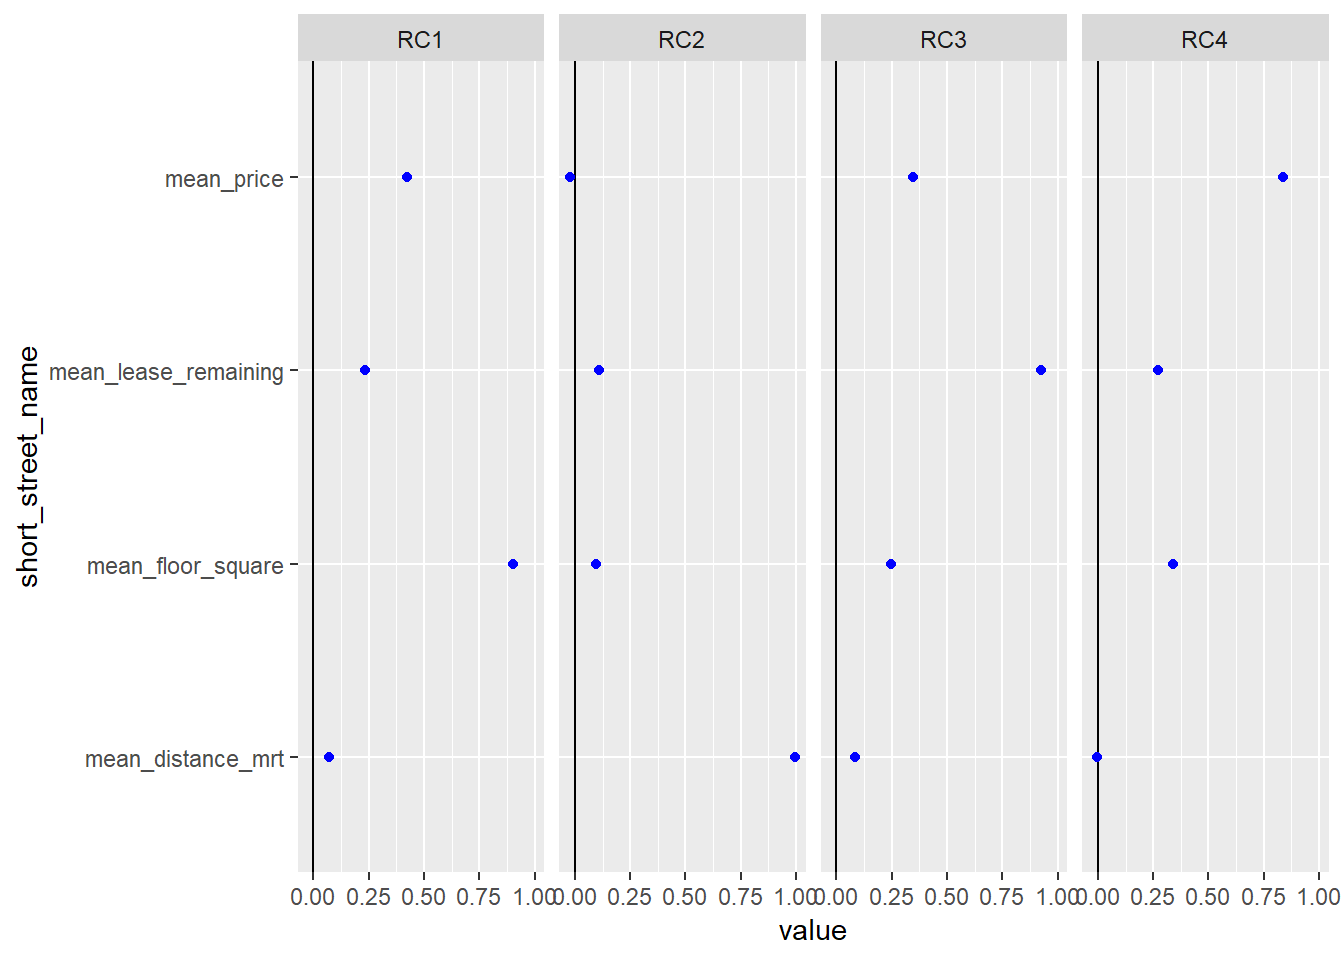
\includegraphics{bookdown-demo_files/figure-latex/unnamed-chunk-40-1.pdf}
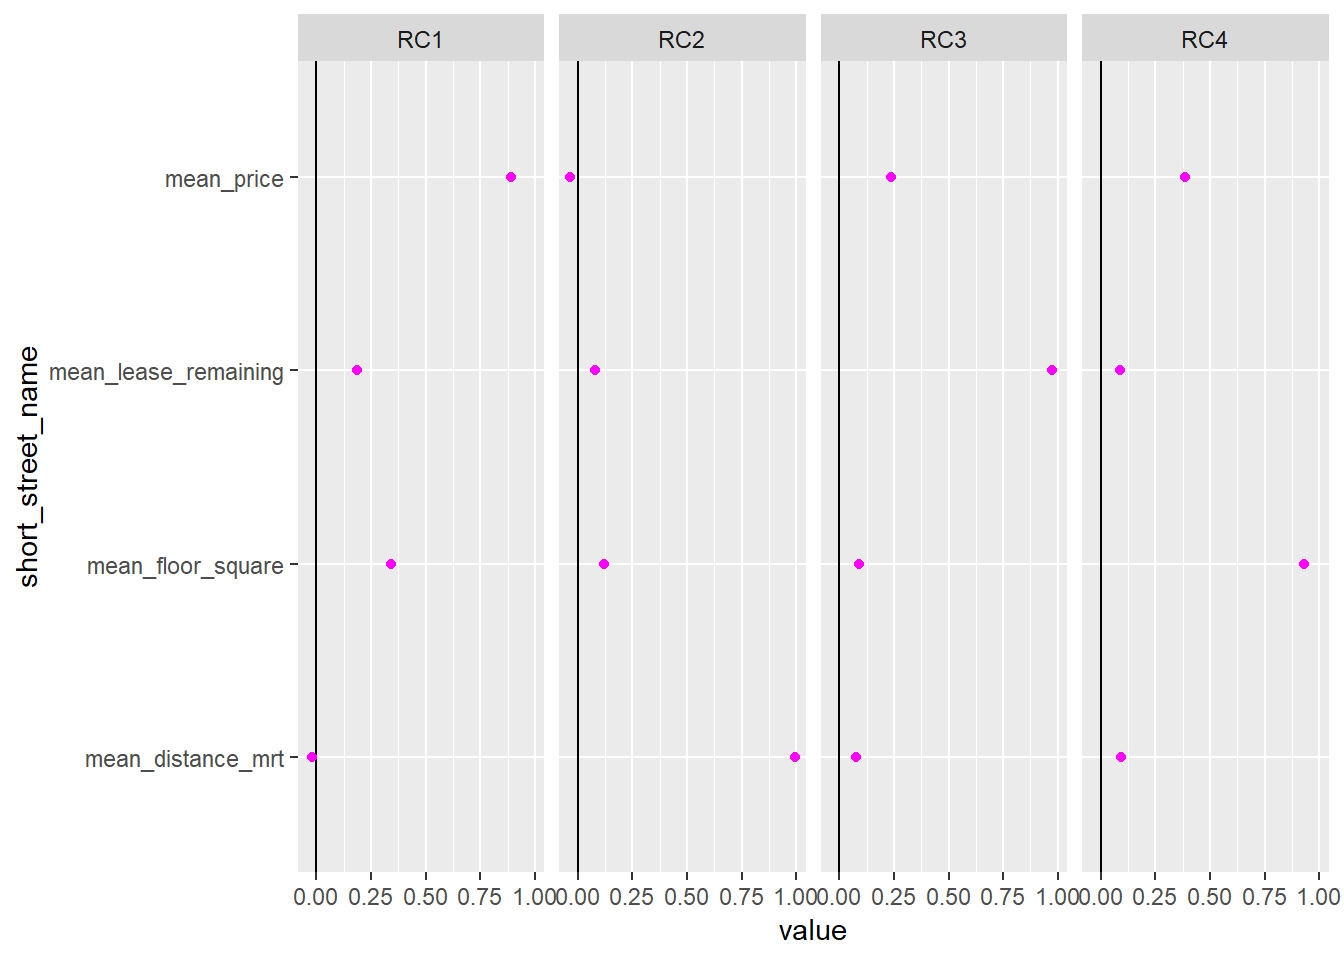
\includegraphics{bookdown-demo_files/figure-latex/unnamed-chunk-41-1.pdf}

By observing all three plots, RC2 and RC3 looks similar which is a good
way to compare across period. Hence, three plots are made to show how
the streets are clustered using RC2 and RC3. This is then followed by a
k means clustering plots for all four factors. This will provide two
ways of looking at the data, RC2 and RC3 as well as RC1 and RC2.

\begin{Shaded}
\begin{Highlighting}[]
\NormalTok{fa <-}\StringTok{ }\NormalTok{tamp_block_p1 }\OperatorTok\StringTok{ }
\StringTok{  }\KeywordTok{column_to_rownames}\NormalTok{(}\DataTypeTok{var =} \StringTok{"short_street_name"}\NormalTok{) }\OperatorTok
\StringTok{  }\KeywordTok{select}\NormalTok{(}\OperatorTok{-}\NormalTok{period) }\OperatorTok\StringTok{ }
\StringTok{  }\KeywordTok{principal}\NormalTok{(}\DataTypeTok{nfactors =} \DecValTok{4}\NormalTok{, }\DataTypeTok{rotate =} \StringTok{"varimax"}\NormalTok{) }\OperatorTok\StringTok{ }
\StringTok{  }\KeywordTok{pluck}\NormalTok{(}\StringTok{'scores'}\NormalTok{) }\OperatorTok\StringTok{ }
\StringTok{  }\KeywordTok{unclass}\NormalTok{() }\OperatorTok\StringTok{ }
\StringTok{  }\KeywordTok{as_tibble}\NormalTok{(}\DataTypeTok{rownames =} \StringTok{"short_street_name"}\NormalTok{)}
  

\NormalTok{fa }\OperatorTok
\StringTok{  }\KeywordTok{ggplot}\NormalTok{(}\KeywordTok{aes}\NormalTok{(}\DataTypeTok{x =}\NormalTok{ RC2, }\DataTypeTok{y =}\NormalTok{ RC3)) }\OperatorTok{+}\StringTok{ }\KeywordTok{geom_text}\NormalTok{(}\KeywordTok{aes}\NormalTok{(}\DataTypeTok{label =}\NormalTok{ short_street_name))}
\end{Highlighting}
\end{Shaded}

\begin{figure}
\centering
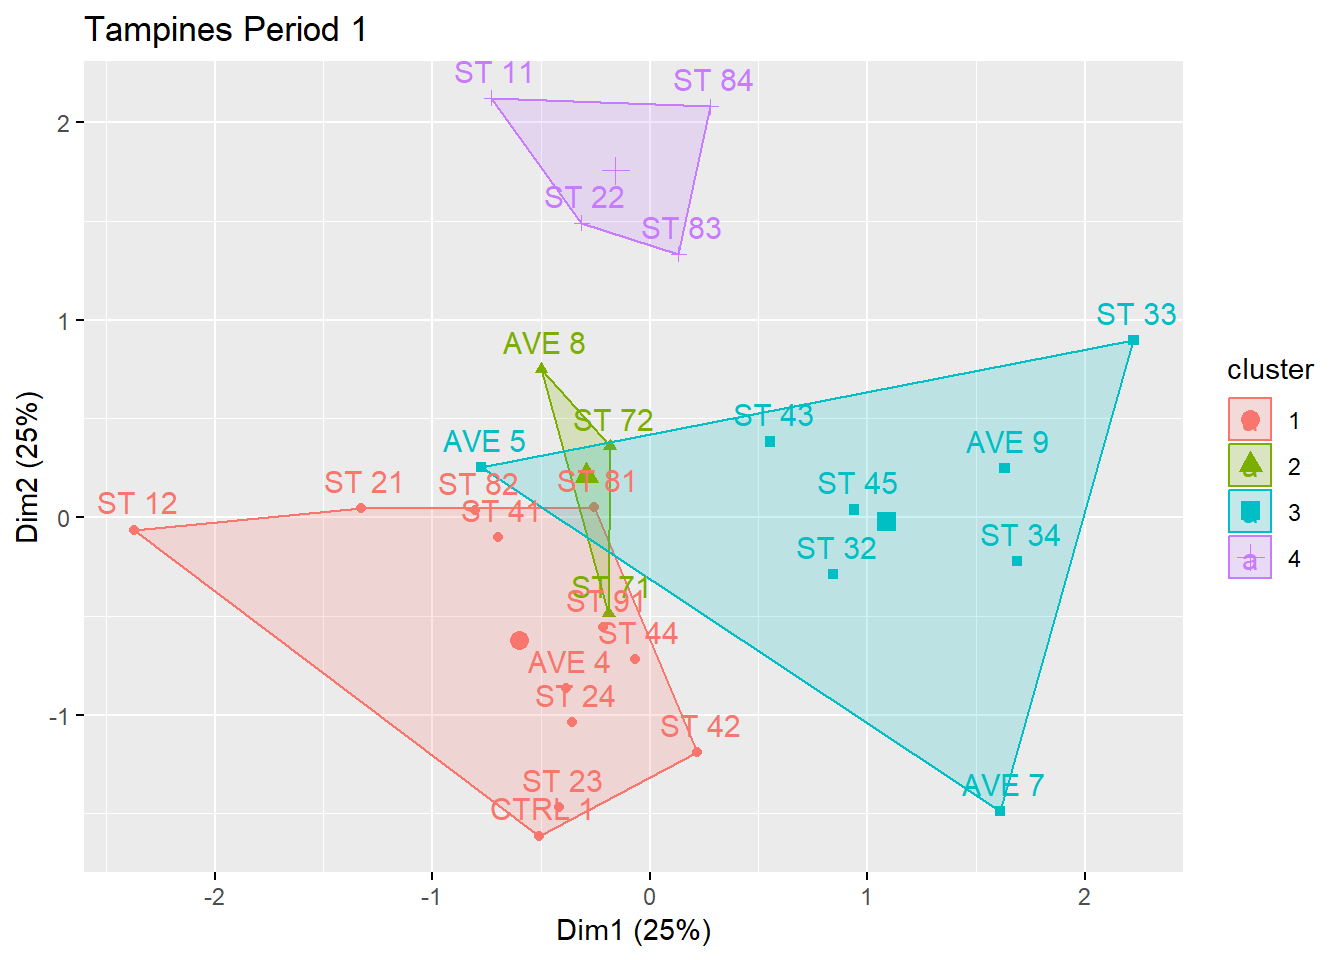
\includegraphics{bookdown-demo_files/figure-latex/unnamed-chunk-42-1.pdf}
\caption{\label{fig:unnamed-chunk-42}\label{fig:figs}Factor Analysis Period
1}
\end{figure}

\begin{Shaded}
\begin{Highlighting}[]
\KeywordTok{set.seed}\NormalTok{(}\DecValTok{1234}\NormalTok{)}

\NormalTok{cluster_data <-}\StringTok{ }\NormalTok{fa }\OperatorTok\StringTok{ }\CommentTok{# remove planning_area column so we are left with only 'data' columns}
\StringTok{  }\KeywordTok{column_to_rownames}\NormalTok{(}\DataTypeTok{var =} \StringTok{"short_street_name"}\NormalTok{)}

\NormalTok{kmeans_clusters <-}\StringTok{ }\KeywordTok{kmeans}\NormalTok{(cluster_data, }\DataTypeTok{centers =} \DecValTok{4}\NormalTok{, }\DataTypeTok{nstart =} \DecValTok{50}\NormalTok{)}

\NormalTok{kmeans_clusters}
\end{Highlighting}
\end{Shaded}

\begin{verbatim}
## K-means clustering with 4 clusters of sizes 12, 3, 8, 4
## 
## Cluster means:
##          RC1        RC3        RC2        RC4
## 1 -0.4020473 -0.4447678 -0.6274196 -0.4702097
## 2  0.4625298  1.2834533  1.1413307 -1.5865209
## 3  0.7544959  0.6008555 -0.2033782  0.9231409
## 4 -0.6497472 -0.8299978  1.4330172  0.7542379
## 
## Clustering vector:
##   AVE 4   AVE 5   AVE 7   AVE 8   AVE 9  CTRL 1   ST 11   ST 12   ST 21 
##       1       3       3       2       3       1       4       1       1 
##   ST 22   ST 23   ST 24   ST 32   ST 33   ST 34   ST 41   ST 42   ST 43 
##       4       1       1       3       3       3       1       1       3 
##   ST 44   ST 45   ST 71   ST 72   ST 81   ST 82   ST 83   ST 84   ST 91 
##       1       3       2       2       1       1       4       4       1 
## 
## Within cluster sum of squares by cluster:
## [1] 18.151954  1.960164 23.805472  1.824574
##  (between_SS / total_SS =  56.0 %)
## 
## Available components:
## 
## [1] "cluster"      "centers"      "totss"        "withinss"    
## [5] "tot.withinss" "betweenss"    "size"         "iter"        
## [9] "ifault"
\end{verbatim}

\begin{Shaded}
\begin{Highlighting}[]
\KeywordTok{fviz_cluster}\NormalTok{(kmeans_clusters, }\DataTypeTok{data =}\NormalTok{ cluster_data, }\DataTypeTok{main =} \StringTok{"Tampines Period 1"}\NormalTok{)}
\end{Highlighting}
\end{Shaded}

\begin{figure}
\centering
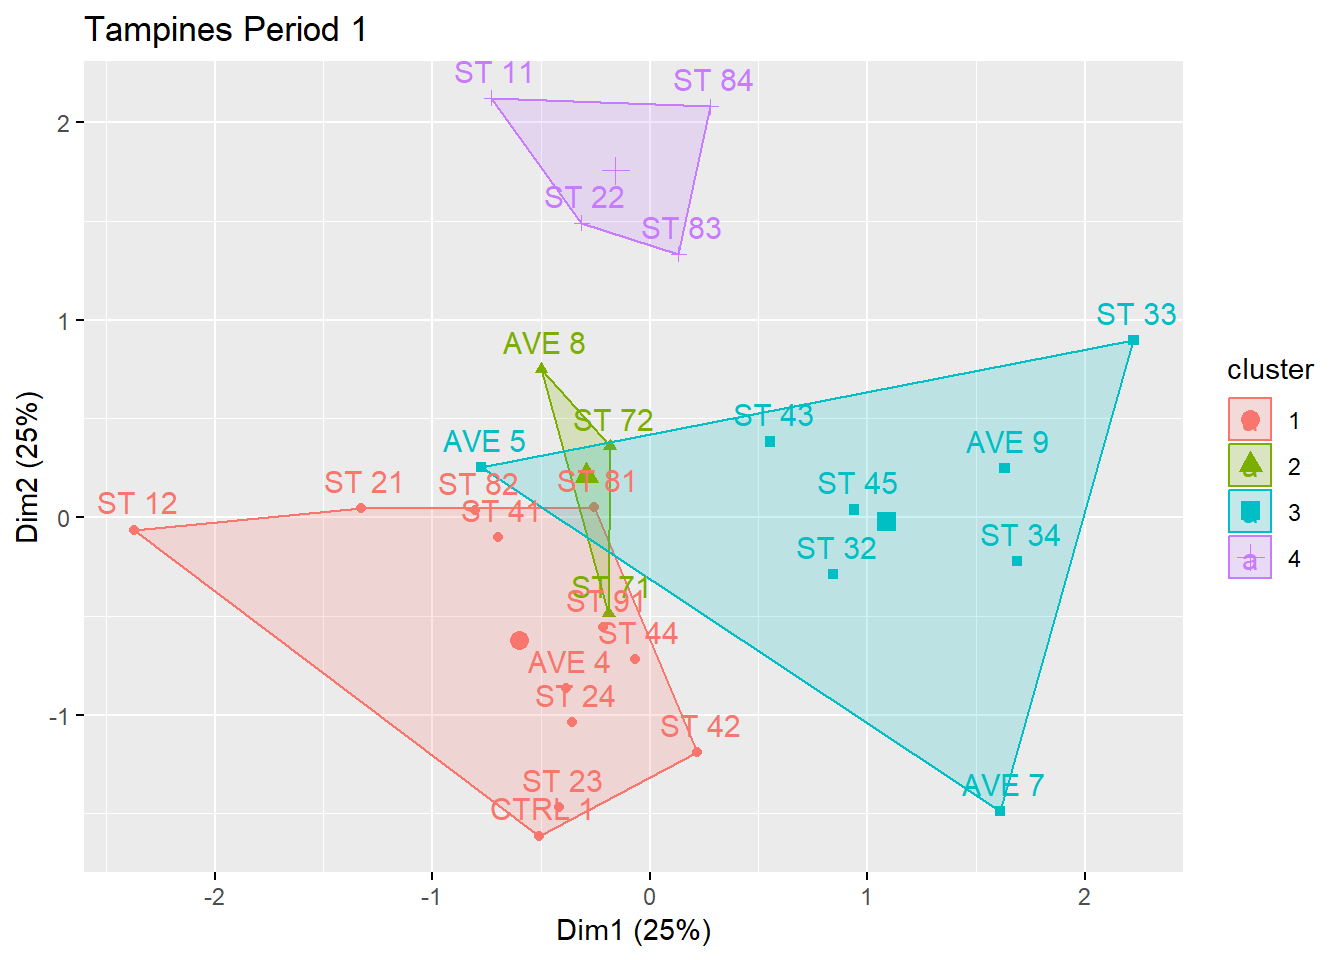
\includegraphics{bookdown-demo_files/figure-latex/unnamed-chunk-44-1.pdf}
\caption{\label{fig:unnamed-chunk-44}\label{fig:figs}K Means Plot Period 1}
\end{figure}

\begin{Shaded}
\begin{Highlighting}[]
\KeywordTok{fviz_nbclust}\NormalTok{(cluster_data, kmeans, }\DataTypeTok{method =} \StringTok{"wss"}\NormalTok{)}
\end{Highlighting}
\end{Shaded}

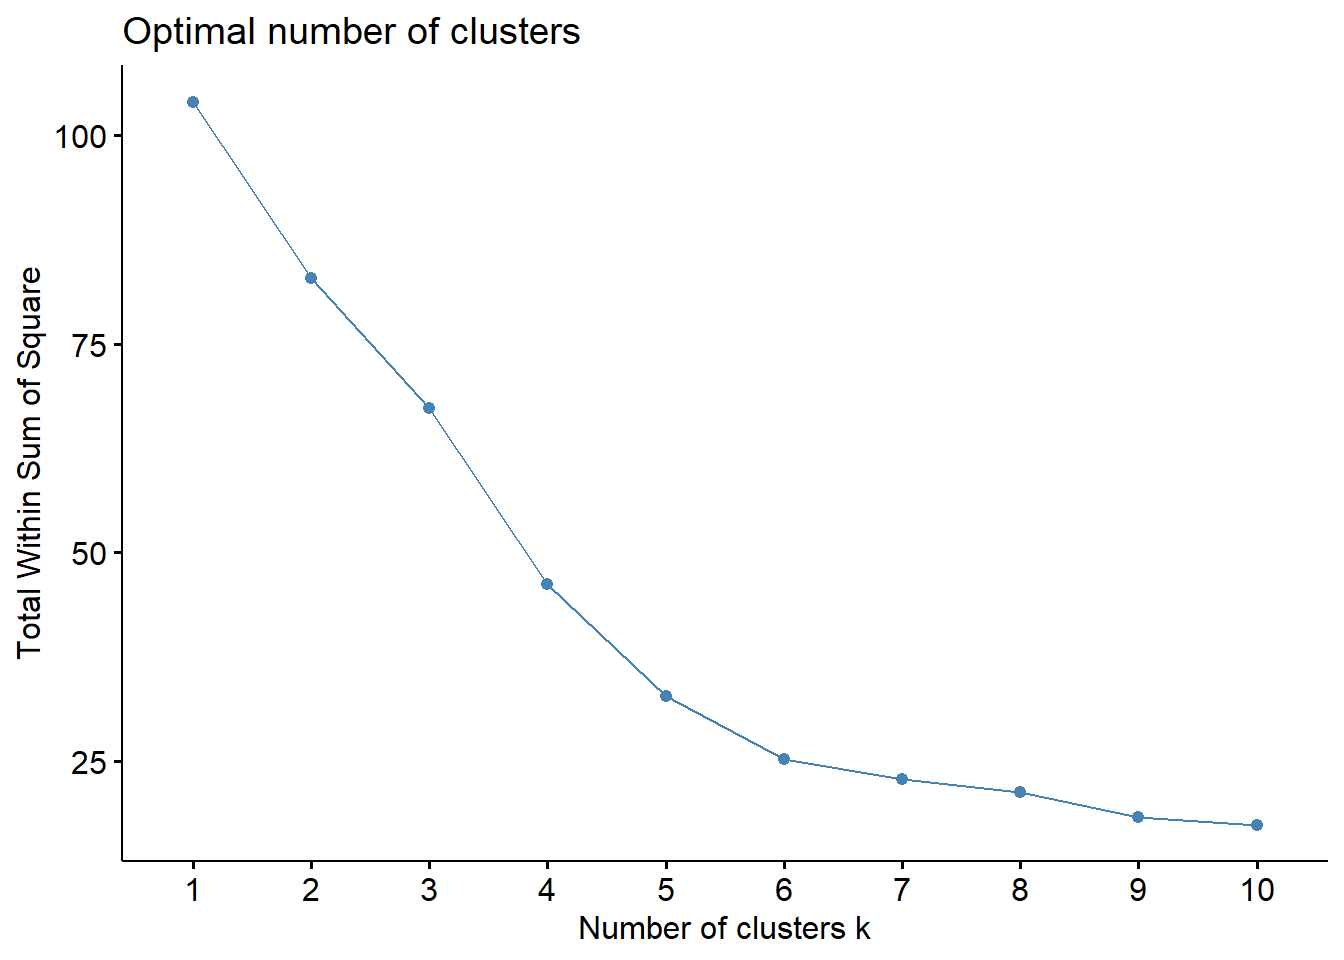
\includegraphics{bookdown-demo_files/figure-latex/unnamed-chunk-45-1.pdf}
A note on determining the number of clusters by identifying the shoulder
from the chart and 4 is a decent number to work with.

\begin{Shaded}
\begin{Highlighting}[]
\NormalTok{fa2 <-}\StringTok{ }\NormalTok{tamp_block_p2 }\OperatorTok\StringTok{ }
\StringTok{  }\KeywordTok{column_to_rownames}\NormalTok{(}\DataTypeTok{var =} \StringTok{"short_street_name"}\NormalTok{) }\OperatorTok
\StringTok{  }\KeywordTok{select}\NormalTok{(}\OperatorTok{-}\NormalTok{period) }\OperatorTok\StringTok{ }
\StringTok{  }\KeywordTok{principal}\NormalTok{(}\DataTypeTok{nfactors =} \DecValTok{4}\NormalTok{, }\DataTypeTok{rotate =} \StringTok{"varimax"}\NormalTok{) }\OperatorTok\StringTok{ }
\StringTok{  }\KeywordTok{pluck}\NormalTok{(}\StringTok{'scores'}\NormalTok{) }\OperatorTok\StringTok{ }
\StringTok{  }\KeywordTok{unclass}\NormalTok{() }\OperatorTok\StringTok{ }
\StringTok{  }\KeywordTok{as_tibble}\NormalTok{(}\DataTypeTok{rownames =} \StringTok{"short_street_name"}\NormalTok{)}
\end{Highlighting}
\end{Shaded}

\begin{Shaded}
\begin{Highlighting}[]
\NormalTok{fa2 }\OperatorTok
\StringTok{  }\KeywordTok{ggplot}\NormalTok{(}\KeywordTok{aes}\NormalTok{(}\DataTypeTok{x =}\NormalTok{ RC2, }\DataTypeTok{y =}\NormalTok{ RC3)) }\OperatorTok{+}\StringTok{ }\KeywordTok{geom_text}\NormalTok{(}\KeywordTok{aes}\NormalTok{(}\DataTypeTok{label =}\NormalTok{ short_street_name))}
\end{Highlighting}
\end{Shaded}

\begin{figure}
\centering
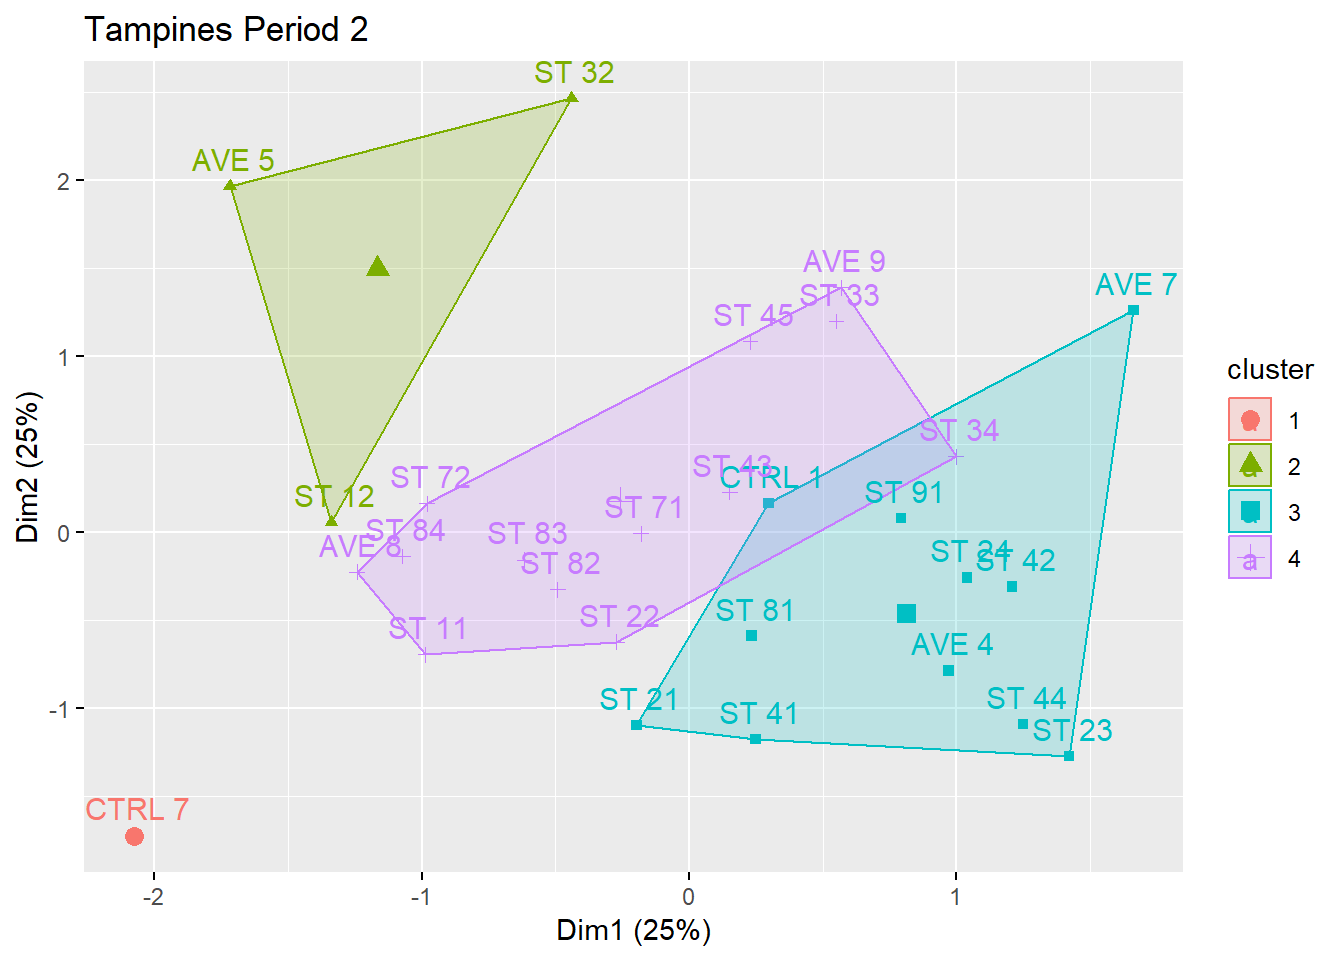
\includegraphics{bookdown-demo_files/figure-latex/unnamed-chunk-47-1.pdf}
\caption{\label{fig:unnamed-chunk-47}\label{fig:figs}Factor Analysis Period
2}
\end{figure}

\begin{Shaded}
\begin{Highlighting}[]
\KeywordTok{fviz_cluster}\NormalTok{(kmeans_clusters2, }\DataTypeTok{data =}\NormalTok{ cluster_data2, }\DataTypeTok{main =} \StringTok{"Tampines Period 2"}\NormalTok{)}
\end{Highlighting}
\end{Shaded}

\begin{figure}
\centering
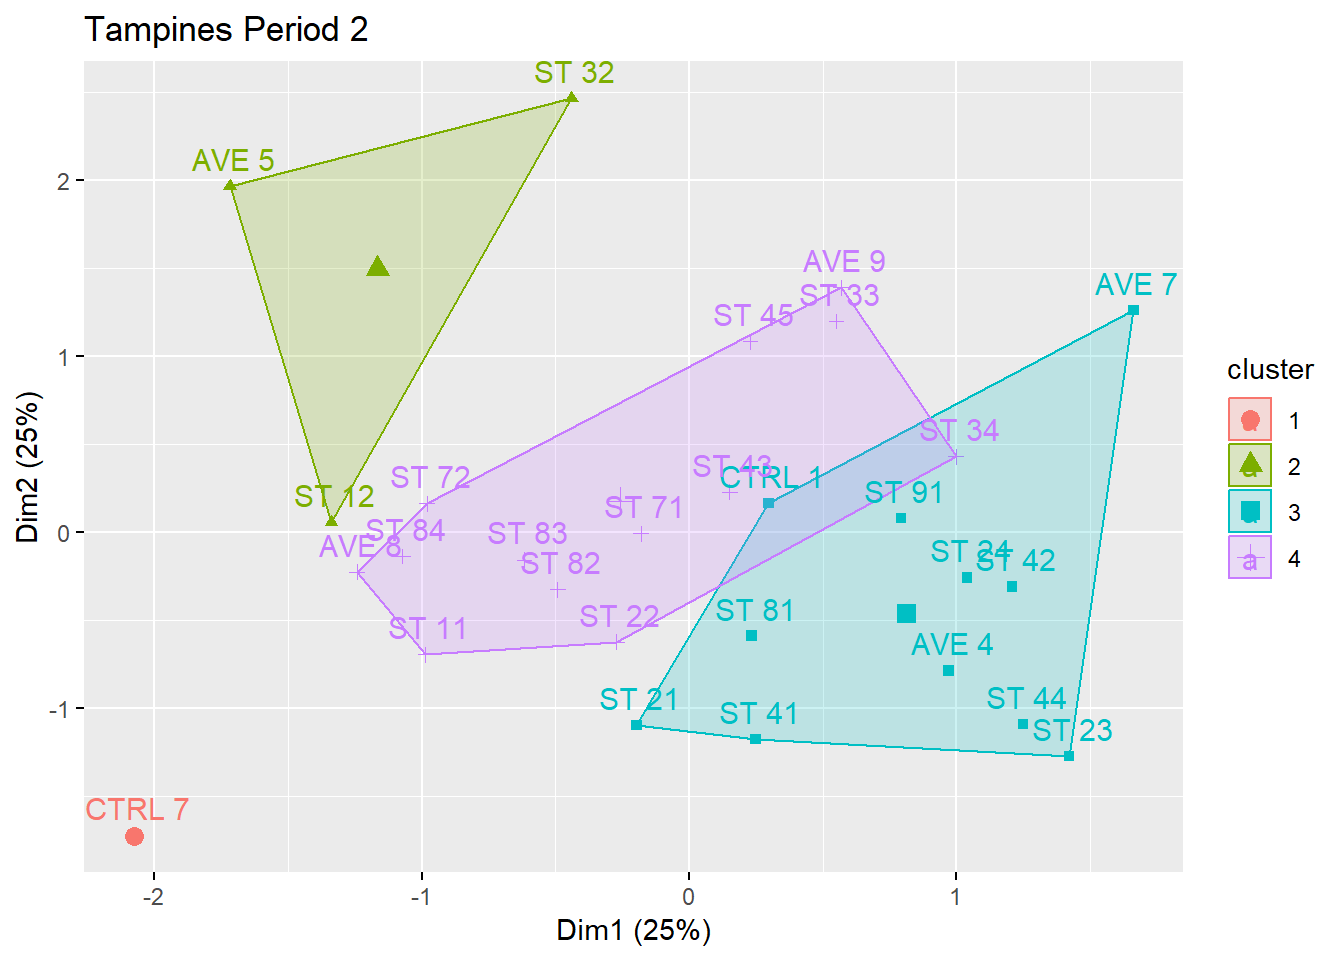
\includegraphics{bookdown-demo_files/figure-latex/unnamed-chunk-49-1.pdf}
\caption{\label{fig:unnamed-chunk-49}\label{fig:figs}K Means Period 2}
\end{figure}

\begin{Shaded}
\begin{Highlighting}[]
\NormalTok{fa3 <-}\StringTok{ }\NormalTok{tamp_block_p3 }\OperatorTok\StringTok{ }
\StringTok{  }\KeywordTok{column_to_rownames}\NormalTok{(}\DataTypeTok{var =} \StringTok{"short_street_name"}\NormalTok{) }\OperatorTok
\StringTok{  }\KeywordTok{select}\NormalTok{(}\OperatorTok{-}\NormalTok{period) }\OperatorTok\StringTok{ }
\StringTok{  }\KeywordTok{principal}\NormalTok{(}\DataTypeTok{nfactors =} \DecValTok{4}\NormalTok{, }\DataTypeTok{rotate =} \StringTok{"varimax"}\NormalTok{) }\OperatorTok\StringTok{ }
\StringTok{  }\KeywordTok{pluck}\NormalTok{(}\StringTok{'scores'}\NormalTok{) }\OperatorTok\StringTok{ }
\StringTok{  }\KeywordTok{unclass}\NormalTok{() }\OperatorTok\StringTok{ }
\StringTok{  }\KeywordTok{as_tibble}\NormalTok{(}\DataTypeTok{rownames =} \StringTok{"short_street_name"}\NormalTok{)}
\end{Highlighting}
\end{Shaded}

\begin{Shaded}
\begin{Highlighting}[]
\NormalTok{fa3 }\OperatorTok
\StringTok{  }\KeywordTok{ggplot}\NormalTok{(}\KeywordTok{aes}\NormalTok{(}\DataTypeTok{x =}\NormalTok{ RC2, }\DataTypeTok{y =}\NormalTok{ RC3)) }\OperatorTok{+}\StringTok{ }\KeywordTok{geom_text}\NormalTok{(}\KeywordTok{aes}\NormalTok{(}\DataTypeTok{label =}\NormalTok{ short_street_name))}
\end{Highlighting}
\end{Shaded}

\begin{figure}
\centering
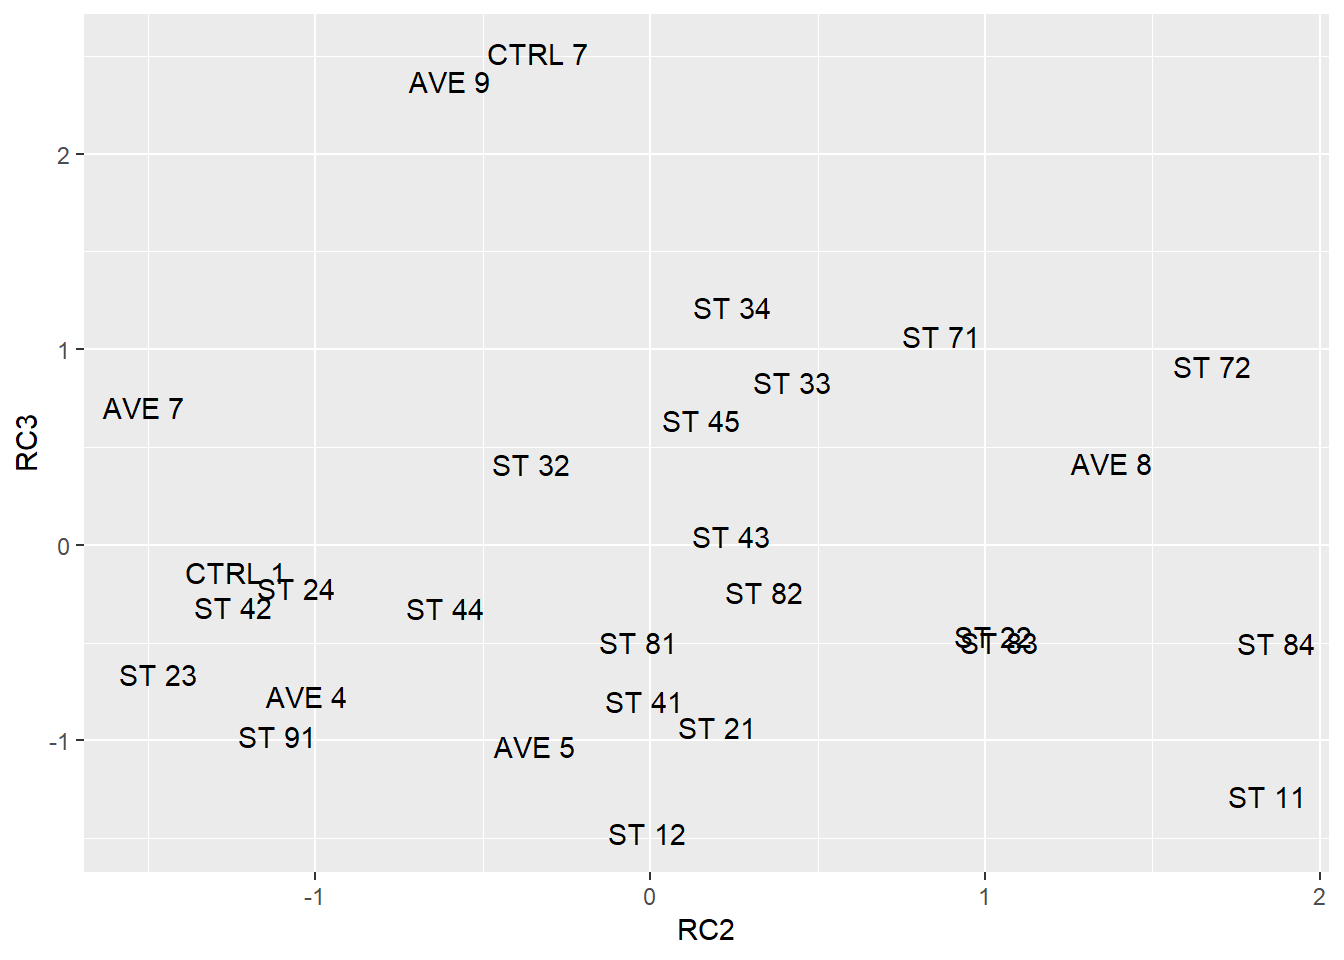
\includegraphics{bookdown-demo_files/figure-latex/unnamed-chunk-51-1.pdf}
\caption{\label{fig:unnamed-chunk-51}\label{fig:figs}Factor Analysis Period
3}
\end{figure}

\begin{verbatim}
## K-means clustering with 4 clusters of sizes 8, 1, 13, 6
## 
## Cluster means:
##          RC4        RC3         RC2         RC1
## 1  0.7405699  0.9106619 -0.07880494 -0.65241104
## 2 -1.6859694  2.5136703 -0.34803984  3.46312336
## 3 -0.2034392 -0.6445917 -0.59886215  0.18052291
## 4 -0.2656466 -0.2365454  1.46061455 -0.09843881
## 
## Clustering vector:
##   AVE 4   AVE 5   AVE 7   AVE 8   AVE 9  CTRL 1  CTRL 7   ST 11   ST 12 
##       3       3       1       4       1       3       2       4       3 
##   ST 21   ST 22   ST 23   ST 24   ST 32   ST 33   ST 34   ST 41   ST 42 
##       3       4       3       3       1       1       1       3       3 
##   ST 43   ST 44   ST 45   ST 71   ST 72   ST 81   ST 82   ST 83   ST 84 
##       1       3       1       1       4       3       3       4       4 
##   ST 91 
##       3 
## 
## Within cluster sum of squares by cluster:
## [1] 17.687999  0.000000 22.978607  6.938138
##  (between_SS / total_SS =  55.9 %)
## 
## Available components:
## 
## [1] "cluster"      "centers"      "totss"        "withinss"    
## [5] "tot.withinss" "betweenss"    "size"         "iter"        
## [9] "ifault"
\end{verbatim}

\begin{Shaded}
\begin{Highlighting}[]
\KeywordTok{fviz_cluster}\NormalTok{(kmeans_clusters3, }\DataTypeTok{data =}\NormalTok{ cluster_data3, }\DataTypeTok{main =} \StringTok{"Tampines Period 3"}\NormalTok{)}
\end{Highlighting}
\end{Shaded}

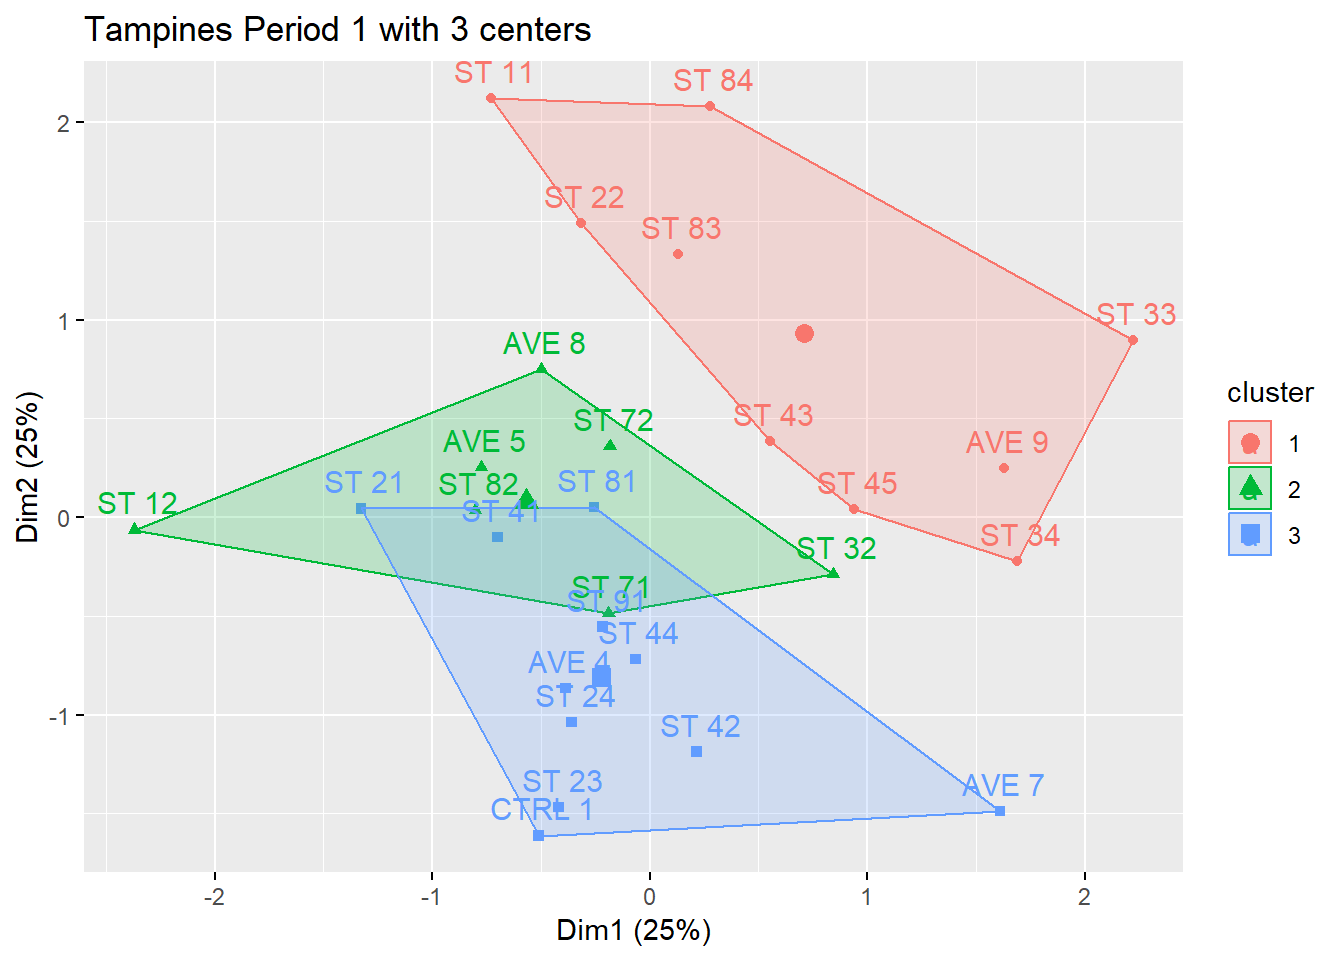
\includegraphics{bookdown-demo_files/figure-latex/unnamed-chunk-53-1.pdf}
For RC2 and RC3, a street that has a major change in relative positions
is Ave 9. Ave 9 was similar to St 32 in period 1 and 2 and then moved to
near to Ctrl 7. St 83 and St 22 moved closer. There is a change in
scales with Ctrl 7 from Period 2. Based on RC2 and RC3, the positions
are clustered and remain similar despite the completion of the new MRT
stations. This shows some stability and that distance to MRT and lease
remaining has little impact. This is supported by the small coefficients
in the log-linear regression model.

In k means clustering, the outlier Ctrl 7 has skewed the data and thus
period 2 and period 3 cluster plot has shifted mostly to a corner of the
graph away from the other points. Ctrl 7 has Design Build and Sell
Scheme (DBSS) flats which is in-between a executive condominium and
regular HDB flats, translating to higher resale price. The average lease
remaining for DBSS is high at 90 years and floor area is 108 square
metres, which also deviate from Tampines average.

By observing the movements across the clusters as adjusted with the best
fit of cluster numbers since the clusters are arbituary across time
periods, there are 16 streets that cluster remains unchanged, while the
rest of the 12 changed. To compare 3 clusters easily across 3 periods, k
means with 3 clusters is performed.

\begin{Shaded}
\begin{Highlighting}[]
\NormalTok{kmeans_clusters1 <-}\StringTok{ }\KeywordTok{kmeans}\NormalTok{(cluster_data, }\DataTypeTok{centers =} \DecValTok{3}\NormalTok{, }\DataTypeTok{nstart =} \DecValTok{50}\NormalTok{)}

\NormalTok{kmeans_clusters1}
\end{Highlighting}
\end{Shaded}

\begin{verbatim}
## K-means clustering with 3 clusters of sizes 9, 7, 11
## 
## Cluster means:
##          RC1        RC3        RC2        RC4
## 1 -0.2192364  0.1524827  0.7200150  0.9307781
## 2  1.1166228  0.1141529  0.4380098 -0.8788598
## 3 -0.5312029 -0.1974013 -0.8678367 -0.2022713
## 
## Clustering vector:
##   AVE 4   AVE 5   AVE 7   AVE 8   AVE 9  CTRL 1   ST 11   ST 12   ST 21 
##       3       2       3       2       1       3       1       2       3 
##   ST 22   ST 23   ST 24   ST 32   ST 33   ST 34   ST 41   ST 42   ST 43 
##       1       3       3       2       1       1       3       3       1 
##   ST 44   ST 45   ST 71   ST 72   ST 81   ST 82   ST 83   ST 84   ST 91 
##       3       1       2       2       3       2       1       1       3 
## 
## Within cluster sum of squares by cluster:
## [1] 19.57024 28.51670 14.97225
##  (between_SS / total_SS =  39.4 %)
## 
## Available components:
## 
## [1] "cluster"      "centers"      "totss"        "withinss"    
## [5] "tot.withinss" "betweenss"    "size"         "iter"        
## [9] "ifault"
\end{verbatim}

\begin{Shaded}
\begin{Highlighting}[]
\KeywordTok{fviz_cluster}\NormalTok{(kmeans_clusters1, }\DataTypeTok{data =}\NormalTok{ cluster_data, }\DataTypeTok{main =} \StringTok{"Tampines Period 1 with 3 centers"}\NormalTok{)}
\end{Highlighting}
\end{Shaded}

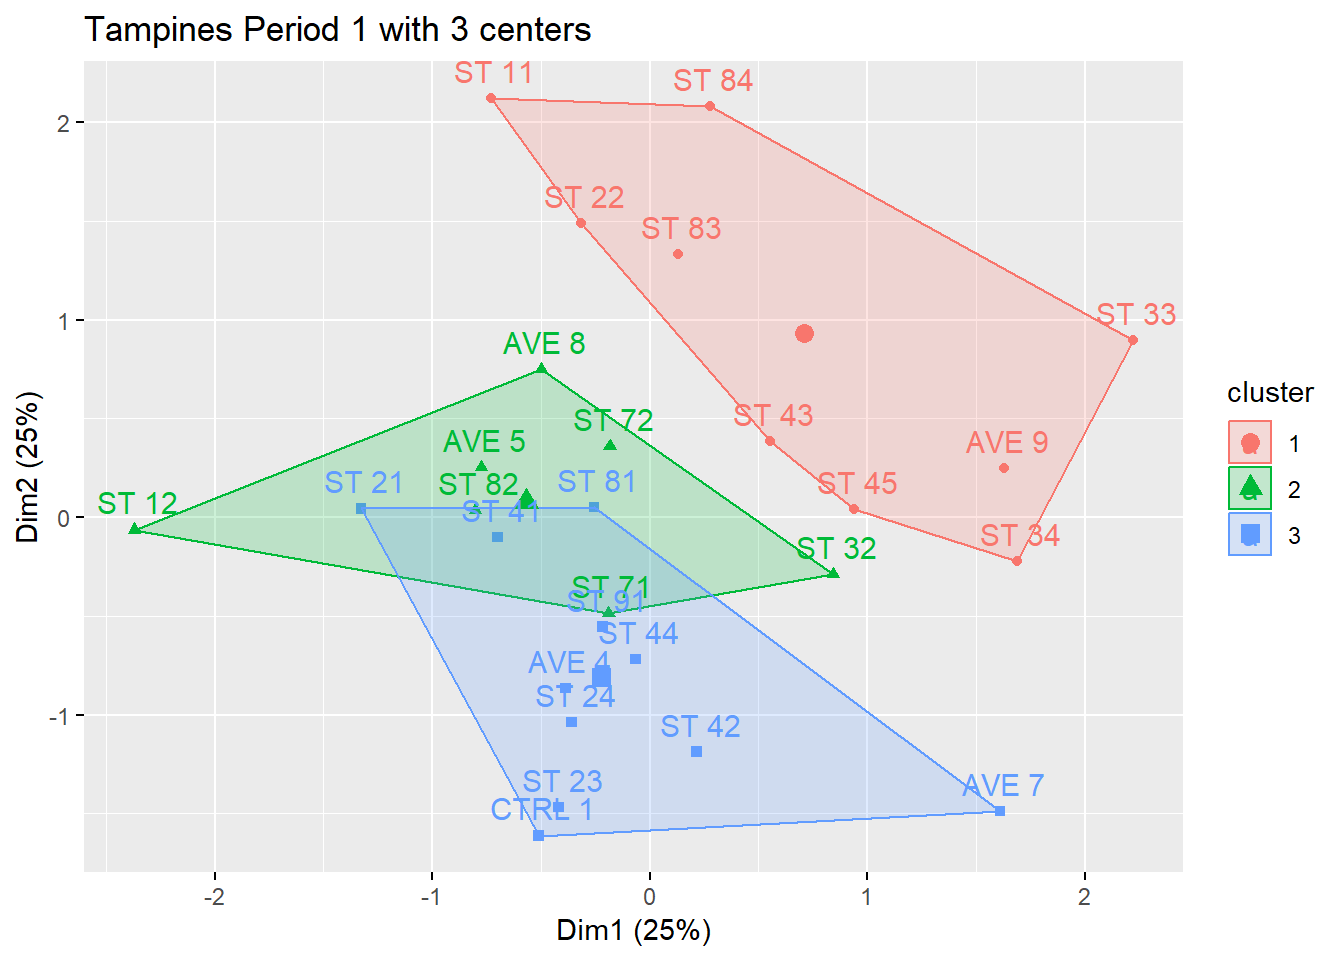
\includegraphics{bookdown-demo_files/figure-latex/unnamed-chunk-55-1.pdf}
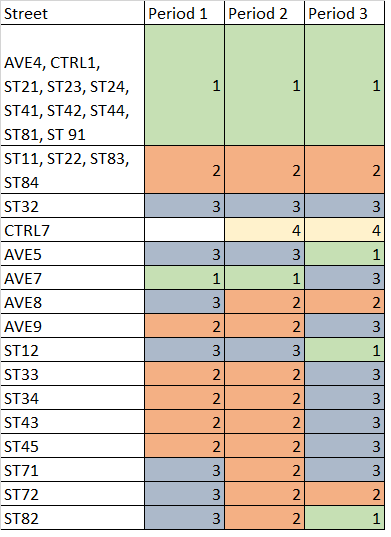
\includegraphics{table cluster.png} With Ctrl 7 fixed at cluster 4
according to the table, the clusters that did not change will be the
reference points for comparison. Ave 5 and St 12 was similar to St 32
but changed in period 3 to the majority because larger flats were sold
for St 12 in period 3 and Ave 5 has the new Tampines Hub that may
impacted the flat price. Ave 5 is en-circling from Industrial Ave 3 to
Simei, hence the effect is not easily found on geographic space. Ave 7
moved from being like the majority to St 32 in period 3 is likely the
opening of Tampines East as the eastern part of St 32 lies the MRT
station. Also, St 32 and Ave 7 are geographically close. Ave 8 and St 72
in period 2 becomes similar to St 11, St 22, St 83 and St 84 where they
are further from the MRT station and near Angsana Primary School or
Junyuan Secondary School. AVe 8 is near Springfield Secondary and St 72
is near Poi Ching exhibit similar characteristics of near a school that
might explains the similarity. These streets are slightly far from the
MRT station too. AVE9, ST33, ST34, ST43, ST45 are located at the
northern part of Tampines which could be geographically similar and
hence cluster groups are the same for 3 periods. A change in period 3
could be Tampines East MRT effect which is perpendicular to St 32 -
period 3 reference point.

There are some new findings from clustering that can be attributed by
the 4 factors or other factors not considered in this study. Clustering
is a useful tool to do other forms of research and uncover differen
angles.

\chapter{Discussion}\label{discussion}

\section{Strengths}\label{strengths}

The high R-square values and residuals which are quite normalised
presents a good case of how HDB resale flat prices can be modelled. For
cluster analysis, it opens up the opportunity to examine street level
trends using the chosen numerical summaries.

\section{Weaknesses}\label{weaknesses}

For regression, parks and primary schools did not have a significant
effect on price, that was not as what I have expected. It could have
other variables or reasons to better estimate the coefficients. The
study consider 1km as the cut-off distance, which can be amended to 0.5,
1 and 1.5km for analysis. For clustering, the choice of street level may
not be a good perspective.

\section{Possible Further Studies}\label{possible-further-studies}

The study focus on local level price dynamics of HDB prices by choosing
an estate in the East and Northwest of Singapore. Tampines as one of the
five other emerging hubs (Woodlands, Changi, Jurong Lake, Punggol
Digital) to decentralise Singapore is a good motivation to study the
trend. An extended study can be done to explore the all the stations on
the Downtown Line. This could be compared to other opening of MRT is the
recent decades such as the Circle Line. Thomson-East Coast Line could
have similar trajectory based on the variables provided by DataGov.

Bukit Panjang has an LRT station connected from Choa Chu Kang to Bukit
Panjang which was not considered in this study. The bus system acts
compliments the MRT in other estates which hig frequency that may not be
an important. A comparsion with Punggol and Sengkang would be
appropriate since they have an existing LRT line.

Private properties are not considered and the impact of new MRT station
affects the real estate values for speculative and investment returns.

K Means on Bukit Panjang can be done to find patterns. Also, other
variables can be included and then dimensional reduction can be done to
sieve out the critical variables that affect resale prices with the
highest impact.

\chapter{Summary}\label{summary}

The project has answered how HDB prices are affected by the opening of a
new MRT station, and the distance to MRT station from the housing unit
is significant. K means clustering has some promising results to examine
the factors that affect the street level.

\bibliography{book.bib,packages.bib}


\end{document}
